% thesis.tex
% This is the main file, which calls up preamble.tex, frontmatter.tex, and thesis.bib as needed.

% Frontmatter shortcuts; note the extra space at the end, which is unfortunately necessary:
\newcommand\myname{Marcello Alves de Sales Junior }
\newcommand\mytitle{Data Persistence for Sensor Networks: A
Taxonomic-Empirical Analysis For Real-World Applications} 
\newcommand\thismonth{December } 
\newcommand\thisyear{2009 }

% Shortcuts (add your own...):
\newcommand{\N}{\mathbb{N}}
\newcommand{\Z}{\mathbb{Z}}
\newcommand{\Q}{\mathbb{Q}}
\newcommand{\R}{\mathbb{R}}
\newcommand{\C}{\mathbb{C}}
\newcommand{\doubleS}{\mathbb{S}}
\newcommand{\vnorm}[1]{\left\|#1\right\|}
\newcommand{\degree}{\ensuremath{^\circ}}
\newcommand{\superscript}[1]{\ensuremath{^{\textrm{#1}}}}
\newcommand{\subscript}[1]{\ensuremath{_{\textrm{#1}}}}
% One of the following two has to be commented out:
%\include{draftpreamble}  % eco-friendly draft version
% preamble.tex, to be used with thesis.tex
% This contains the TeX definitions for layout, style, etc., as well as the first few pages of your thesis: title page, copyright page, approval page, abstract, acknowledgments, tables of contents, tables, and figures.
% The layout commands should give the correct margins according to the graduate division's guidelines

%%%%% TeX class and packages

\documentclass[12pt,oneside]{sfsuthesis}
\usepackage{amsthm,amsmath,amssymb,amsfonts,latexsym,graphicx,enumerate,setspace,verbatim,makeidx,subfigure, multirow, url, soul}
\usepackage[subfigure]{tocloft}
\usepackage{color}                       % For creating colored text and background
%\usepackage{hyperref}                 % For creating hyperlinks in cross
%references
% other possibly useful packages: textcomp,mathrsfs,amscd,epsfig,euscript,cancel

%%%%% Layout
% These numbers might depend on your printer. Check the margins and compare them to the Graduate Division's
% guidelines. If there's something off, try playing with the numbers...
%
% For chapters:
%     Must have a minimum of 1.5in margin on left and 1in on all other sides.  Where there are page numbers
%     (whether on top or bottom), must have one additional inch between the page number and the text, for a
%     total of 2in between the edge of the paper and the text.
% For frontmatter pages:
%     The same margin numbers generally work, except for the Title Page, so you will notice that we use
%     some numbers for \textheight and \footskip right here, and then change them below, right after
%     generating the Title Page.

\pdfpagewidth 8.5in
\pdfpageheight 11in 
\setlength\topmargin{0in}
\setlength\headheight{0in}
\setlength\headsep{0in}
\setlength\textheight{7.7in}
\setlength\textwidth{6.5in}
\setlength\oddsidemargin{0in}
\setlength\evensidemargin{0in}
\setlength\headheight{77pt}
\setlength\headsep{0.25in}

%\hoffset=.5in 
%\oddsidemargin=0in
%\evensidemargin=0in
%\topmargin=0.0in 
%\headheight=0in
%\headsep=1in
%\footskip=.8in
%\textwidth=6.5in
%\textheight=7in

\setcounter{secnumdepth}{3}
\setcounter{tocdepth}{3}

\pagestyle{plain}

\doublespacing

%%%%% Style of theorems, definitions, examples, equations, etc.

\theoremstyle{plain} % Heading is bold, text italic.
\newtheorem{theorem}{Theorem}[chapter]
\newtheorem{lemma}[theorem]{Lemma}
\newtheorem{proposition}[theorem]{Proposition}
\newtheorem{corollary}[theorem]{Corollary}
\newtheorem{conjecture}{Conjecture}[chapter]

\theoremstyle{definition}  % Heading is bold, text is roman
\newtheorem{definition}{Definition}[chapter]
\newtheorem{example}{Example}[chapter]

\theoremstyle{remark}  % Heading is italic, text is roman
\newtheorem*{remark}{Remark}
\newtheorem*{note}{Note}
\newtheorem{claim}{Claim}[chapter]

%%%%% Appendix style

\renewcommand\appendix[1]{
\chapter*{#1}
\addcontentsline{toc}{chapter}{#1}
}

%%%%% Source-Code listings

\usepackage{courier}
\usepackage{color}
\usepackage{xcolor}
\usepackage{listings}

\lstset{commentstyle=\tiny,captionpos=t,tabsize=2,frame=lines,keywordstyle=\color{blue}\tiny,commentstyle=\color{gray}\tiny,stringstyle=\color{red}\tiny,numbers=left,numberstyle=\tiny,breaklines=true,showstringspaces=false,basicstyle=\tiny,emph={label}}

%\definecolor{darkgreen}{named}{green}
%\definecolor{darkblue}{named}{blue}
%\definecolor{darkred}{named}{red}
%\definecolor{grau}{named}{gray}
%\let\Righttorque\relax
%\lstset{
%commentstyle=\itshape\color{darkgreen},
%keywordstyle=\bfseries\color{darkblue},
%stringstyle=\color{darkred},
%extendedchars=true,
%basicstyle=\scriptsize\ttfamily,
%basicstyle=\tiny\ttfamily,
%tabsize=2,
% keywordstyle=\textbf,
%commentstyle=\color{grau},
% stringstyle=\textit,
%numbers=left,
%numberstyle=\tiny,
% für schönen Zeilenumbruch
%breakautoindent = true,
%breakindent = 2em,
%breaklines = true,
%postbreak = ,
%prebreak = \raisebox{-.8ex}[0ex][0ex]{\ensuremath{\lrcorner}},
%prebreak = \raisebox{-.8ex}[0ex][0ex]{\Righttorque},
%showspaces=false, % Keine Leerzeichensymbole
%showtabs=false, % Keine Tabsymbole
%showstringspaces=false,% Leerzeichen in Strings
%}

\usepackage{caption}
\DeclareCaptionFont{white}{\color{white}}
\DeclareCaptionFormat{listing}{\colorbox{gray}{\parbox{\textwidth}{#1#2#3}}}
\captionsetup[lstlisting]{format=listing,labelfont=white,textfont=white}

%% Use fancy chapter headers, with Jos Dingjan's modifications,
%% plus my own tweaks. This style is not part of teTeX,
%% so we are using a local (and renamed) copy.
\usepackage[Lenny]{fncychap}

%Hifens
\usepackage[latin1]{inputenc}
\usepackage[USenglish]{babel}

%Harvard citation style
\usepackage{natbib}
%enhanced items
% http://dante.ctan.org/tex-archive/macros/latex/contrib/enumitem/enumitem.pdf
\usepackage{enumitem}

\begin{document}

\pagenumbering{roman}
\thispagestyle{empty}

\[ \]
\vspace{-1.8in}

\begin{center}
{\mytitle}

\vspace{1.4in}

\singlespace{A thesis presented to the faculty of\\
San Francisco State University\\
In partial fulfillment of\\
The requirements for\\ The degree}

\vspace{.5in}

\singlespace{Master of Science\\ In\\ Computer Science}

\vspace*{\fill}

{by \\[12pt] 
\myname \\[12pt]
San Francisco, California\\[12pt]
\thismonth
\thisyear}
\end{center}

\newpage
\thispagestyle{empty}

$\mbox{}$
\vspace{3in}
\begin{center}
\singlespace{
    Copyright \copyright{} \thisyear by \myname
%    \bigskip
%    All rights reserved. No part of the material protected by this
%    copyright notice may be reproduced or utilized in any form or by any
%    means, electronic or mechanical, including photocopying, recording or
%    by any information storage and retrieval system, without the prior
%    permission of the author.
}
\end{center}

\newpage
\thispagestyle{empty}
\[ \]
\vspace{-1.8in}
\begin{center}
{CERTIFICATION OF APPROVAL}
\end{center}
\vspace{.5in}
\begin{quote}
I certify that I have read {\it \mytitle} by \myname, and that in my opinion
this work meets the criteria for approving a thesis submitted in partial
fulfillment of the requirements for the degree: Master of Science in Computer
Science at San Francisco State University.
\end{quote}

\vspace{1.5in}

\hspace*{\fill}\parbox{3.5in}{
\singlespace{

\hrule{\hspace{3.5in}} \\ 
Prof. Arno Puder, Ph.D.\\
Professor of Computer Science\\
\vspace{1in}
\hrule{\hspace{3.5in}} \\
Prof. Marguerite C. Murphy, Ph.D.\\
Professor of Computer Science

}
}

\newpage
\thispagestyle{empty}
\[ \]
\vspace{-1.8in}
\begin{center}
{\mytitle} \\

\vspace{.5in}

\singlespace{
\myname \\
San Francisco, California \\  
\thisyear \\
}
\end{center}

\vspace{.5in}

%\doublespacing{\noindent
\onehalfspacing{\noindent
Sensor Networks are becoming more and more important to different science
communities because of what they produce: the raw data for different domains.
In order to make use the collected data, researchers may have to dissect the
characteristics of the sensor network in question, regarding different
properties such as the purpose and location of the observed data, as well as
how the data is described. For this reason, this work proposes a set of data
persistence taxonomies based on the state of the art, which can be used to
classify the properties of the produced raw data. In order to evaluate the
proposed taxonomies, this work designs and implements a data persistence
component for NetBEAMS, a modular-based sensor network infrastructure
developed to improve the operation of the SF-BEAMS environmental sensor
network. SF-BEAMS is deployed at the Tiburon Island, California, and managed by
the Department of Biology from SFSU. In this way, based on empirical analysis
regarding proposed taxonomies for the case study, this work selected mongoDB,
a schema-less document-oriented database instead of the traditional use of
relational databases. As a result based of the experiments conducted, this
work proposes a novel use of the Key-Value Pair databases in order tor provide
External of Data-Centric approaches. Similarly, this work also agrees to
related literature that the use of programming languages are better abstraction
than the use of traditional query languages used to extract data from Relational
databases, and therefore, it should be the proposed approach to non-technical
researchers such as the Biologists. Finally, this work proposes different
future works such a data-centric approach using Databasese Shards to store the
collected data and Map Reduce to execute parallel queries over distributed
database nodes.} \vspace*{\fill}
 
\hspace*{\fill}

\noindent
I certify that the Abstract is a correct representation of the content of this thesis.

\vspace{.5in} 

\hrule{\hspace{3.75in}} \\[-10pt]
Chair, Thesis Committee 
\hspace{2.5in}
Date
\onehalfspacing
\newpage
\[ \]
\vspace{-1.8in}
\begin{center}{ACKNOWLEDGMENTS}\end{center}

\vspace{.5in}
\begin{quote}
\noindent
Acknowledgments
\end{quote}

\renewcommand{\contentsname}{\vspace{-1.7in} \begin{center} \normalsize \rm TABLE OF CONTENTS \end{center}}
\renewcommand{\listfigurename}{\vspace{-1.7in} \begin{center} \normalsize \rm LIST OF FIGURES \end{center}}
\renewcommand{\listtablename}{\vspace{-1.7in} \begin{center} \normalsize \rm LIST OF TABLES \end{center}}
\renewcommand{\cftchapfont}{\normalfont}
\renewcommand{\cftchappagefont}{\normalfont}
\renewcommand{\cftchapleader}{\cftdotfill{\cftdotsep}} % formatting commands for table of contents
\renewcommand{\cftsecfont}{\normalfont}
\renewcommand{\cftsecpagefont}{\normalfont}
\renewcommand{\cftsecleader}{\cftdotfill{\cftdotsep}}

\newpage \tableofcontents 
\newpage \listoftables % comment out if you don't use tables
\newpage \listoffigures % comment out if you don't use figures

\newpage
\pagestyle{myheadings}
\pagenumbering{arabic} 
\setcounter{page}{1}
   % final version, formatted according to the Graduate
% Division's guidelines

% Main body of work:

% main.tex, to be used with thesis.tex
% This contains the main work of your thesis.


%\bibliography{thesis}  % uses the references stored in Chapter1Radar.bib

\chapter{Introduction}

Sensor networks are commonly used in different areas for different purposes
such as accurate measurements during scientific research \cite{sn-intro01} and
the general public access such as weather forecast \cite{sn-intro02}. In the
scientific community, they serve as tools to watch the state of the environment
by storing samples of data at particular periods of time. For example, the
NASA Jet Propulsion Laboratory uses the Volcano SensorWeb \cite{sn-ex02}, a
sensor network which aims at collecting data from individual volcanoes in
Alaska and South Pacific to be used with heuristics regarding hazardous
activities. Similarly, the National Data Buoy Center, a division of the
National Oceanic and Atmospheric Administration (NOAA) \cite{sn-ex03},
provides online information from different buoys in different shores around
the world regarding water quality, current information, etc, what
characterizes sensor network for environmental monitoring \cite{sn-ex01}.
Therefore, sensor networks can be seen as an extremely valuable tool
for the scientific and commercial sectors, makeing direct use of the sensor
networks' produced data.

In order to provide access to the collected sensor data, different approaches
can be taken: interrogate sensor devices indirectly by accessing its data in
places called network data sink or simply connect directly to the device. The 
While the latter approach the data is only available in memory as a data
stream, the former approach contains any sort of secondary memory such as a
hard-disk or a flash memory, which are used to archive the collected data.
Along with the location of the collected data from sensors, the the data model
and may also influence in the process of reusing the collected data. In this
way, the lack of a persistence layer for existing sensor networks requires a
deep understanding about its infrastructure, the nature and location of the
collected data, the chosen data model representation, among others. For
instance, how can a data persistence layer safely represent the collected
sensor devices' properties without the necessity of restructuring any existing
data model? Should the end users' skills in database system be taken into
account or the use of programming languages to access the data
\cite{sn-programming-language}? This problem is currently faced by the
department of Biology at San Francisco State University with a marine sensor
network managed by researchers without Computer Science skills. While the data
access may enforce the difficulties, technical issues may also increase while
the implementation of a sensor network such as growth in terms of the number
of sensor devices and, consequently, the number of data produced. Last, but
not least, the way to read the data for reuse is the most striking features of
the sensor network, taking into account the different data formats used by the
primary users of the system. How can individual collected sensor data be
exported to other formats such as spreadsheets in order to be shared among
research peers? For these reasons, the inception of a persistence storage can
be an exceptionally challenging problem to solve.

In view of the fact that the persistence storage of a sensor network imposes
many different challenges, this work proposes the assessment of the current
state of the art for sensor networks in order to provide a data persistence
layer for an existing sensor network. As a matter of fact, this work's first
contribution is the creation of a set of basic taxonomies for data persistence
in sensor networks, proposed to drive an empirical analysis of different
technologies used in the sensor network community. Furthermore, it also takes a
look at different alternatives not yet explored through experiments for a
selected sensor network as a case study. Similarly, this work makes another
novice contribution by suggesting a ``lighter" data model and database
infrastructure that simply captures sensor network devices' observations,
taking into account the non-predictable scalability of its infrastructure, as
well as aspects of the nature of the data such as identity, time and location
of the collected data.

This paper is organized as follows: the next chapter describes the literature
review as the state of art on sensor networks and data persistence, providing
the underlying foundation for the design of taxonomies in data persistence for
sensor networks in chapter 3. Then, chapter 4 examines the selected case study
and its requirements for a persistence layer, whose technology properties are
evaluated in chapter 5 against the developed taxonomies. The culmination of
this work is chapter 6, which details the design and implementation of a data
persistence solution for the selected case study. Likewise, chapter 7 discusses
the solution by presenting the measurements and conducted experiments, and
describes the findings and contributions of this work. Last, but not least,
chapter 8 presents the conclusions of this work, together with the possible
future works not addressed here.

% main.tex, to be used with thesis.tex
% This contains the main work of your thesis.

%\bibliography{thesis}  % uses the references stored in Chapter1Radar.bib

\chapter{State of the Art}

Different aspects related to two major fields of Computer Science have
motivated to the inception of this work. In the perspective of Database
Systems and Distributed Systems, this work seeks a different approach for a
persisting collected data from sensor networks into a storage system that can
be seen as a cluster of distributed databases. Likewise, in the perspective of
Software Engineering, this work adds a major capability to an existing sensor 
network framework, meeting the requirements and interfaces. In general, this 
chapter gives the foundation based on the motivations for the inception of a 
different approach to persisting data using a different data model, covering 
topics that will be referred throughout the following other chapters.

This chapter will first give an overview on different related problems
described in the literature that solved problems related to data modeling and
representation in sensor networks.

\section{Sensor Networks Survey}

Sensor Networks are specialized types of network systems comprised of network 
nodes with specific goals to observe and collect data. Data Persistence in
Sensor Networks, however, depends on the approaches used to store the data,
since data nodes can be located close to the devices in the network or in a
centralized node. In this way, the query process can take place on the network
nodes themselves or on the centralized data sink. The former approach is
generally used when the data is collected at the sensor node on its local
storage \cite{sn-storage01}\cite{sn-storage03}, strategy mainly used to
maximize the sensor's resources while minimizing energy consumption
\cite{sn-storage04}. However, this strategy is used when data archival is not
the primary reason, given the limited resources on the sensor devices. For
this reason, the the latter strategy has been used when the collected data is
primarily archived in a centralized database system for later reuse
\cite{sn-storage02}.

When it comes to data representation, the relational data model
\cite{relational-model} is one of the most used approaches to represent data
in sensor network databases in any of the query processing strategies and, in
most cases, with a modified version of the SQL language \cite{sn-db-newop}.
However, the design of the database system must be done with prior knowledge
of the sensor types when choosing the relational data model, as the database
design must be normalized \cite{db-normalization} for the entities already
identified for the system. For instance, the introduction of a new sensor
device might represent a potential change on the database structure by seeking
a new normalized version of the database structure. In addition to challenges
of maintaining the database schema normalized, the use of Data Provenance
approaches in sensor network data \cite{sn-provenance} usually addresses the
problem related with the lineage of data  and its full history. However, once
the data model is chosen and implemented, one of the most important
non-functional requirements in sensor networks is scalability of the
persistence storage. Since an operational sensor network can produce huge
amounts of data, it must be able to cope with the increase and data load
during data gathering, and yet provide users the same performance during data
retrieval by using different strategies such a data-centric storage
\cite{sn-storage03}.

The following subsections describe classes of characteristis of these types of
sensor networks, with applications on research, industrial or militery.

\subsection{Deployment and Mobility}

Each of the nodes can be deployed in a random way such as being dropped
from an airplane, or in a manual fashion at deliberately chosen geographical 
points \cite{sn-intro01}. Moreover, the deployment can be done as a one-time
event or an iterative way. 

However, nodes can be able to move around the deployed area or be static in
this place. In the case of the degree of the former behaviour, a sensor node
can move occasionally or continuously, being a result of an incidental 
side-effect or a desired property of the device, where they are an automotive
device or attached to another moving object. For this reason, \cite{sn-intro01} 
describes those types of mobility as active or passive.

\subsection{Device Size, Resources, Cost, Energy, Heterogeneity}

Such sensor nodes can be of different sizes, ranging from microscopically small
particles, small devices to bigger ones with a few feet cubic. In addition to
being limited in size, they are also limited in resources and computational
power, forcing their conception limited to have its energy stored in either
batteries or scavenged from solar cells \cite{sn-intro01}.

Since sensor devices range on size and capabilities, the cost for each of the
devices very from hundreds to thousands of dollars, depending on its
functionality, energy utilization, etc. For thie reason, \cite{sn-intro01}
explains that a sensor network may potentially contain similar sensor devices,
as they can contain dissimilar ones from each other, which characterizes the heterogeneity 
of a sensor network by the hardware capabilities such as GPS enabled or having
GSM  network connectivity.

\subsection{Communication Modality, Network Infrastructure, Coverage and
Connectivity}
\label{sec:sn-infrastructure}

Sensor nodes can communicate in different modalities such as radio, diffuse
light, inductive or sound, which may influence on the type of protocols used to
communicate among the nodes, where they can be said to be in an organized
infrastructure or as an ad hoc way \cite{sn-intro01}.

When it comes to the sensor network different organizational infrastructure,
they can differ in types of topology: single-hop, star, networked stars, tree
and graph, where each of them may affect the characteristics of the network as it 
may also influence on data gathering and routing mechanisms. While in a
single-hop sensor network there are only two levels of sensor connectivity, the
tree, graph or networked stars networks uses communications among the network
hosts for data communication.

Last, but not least, sensor networks may be influenced its coverage designed in
its purpose, its size in terms of number of nodes and its relating lifetime. As
sensors are deployed in different areas, they can be distributed in a sparse or
dense way, yet providing necessary coverage for the environment. However, 
considering that sensor devices are very likely to constant failures, projects 
have provided redundant nodes \cite{sn-intro01}. This degree of coverage also 
influences on the connectivity of the sensor nodes, where they can be
considered connected when a connection is available at all times. On the other
hand, nodes can communicate with other nodes in an intermittent way or sporadic
way. In the former, the sensor node is partitioned, while in the latter the
nodes are isolated most of the time and communicates at certain moments in
time.

\subsection{Network Size, Lifetime and Quality-Of-Service}

Similar to the degree of coverage of the sensor network is the number of
sensor nodes deployed in the network, where they can be in the order of
dozens, hundreds or even thousand of nodes \cite{sn-intro01}.

The application of the sensor network determines how long the sensor
network may be exist. For example, the lifetime of an environmental sensor
networks \cite{sn-ex01} may be not determined since its service serves in a
regular basis, whereas the lifetime of a sensor network to determine the number
of people in an event is limited to the event. 

Finally, the design of sensor networks can be related to the constraints
related to quality-of-service (QoS) such as real-time delivery within certain
period of time or robustness such as maintaining data alive even though there
a communication link is not available \cite{sn-intro02}.

\section{Persistence Storage for Sensor Networks}

The most important purpose of a sensor network is related to its main product:
the use of the raw data. Data collection in sensor networks is directly
dependent on the specifications of the sensor network, its routing mechanisms
and the final destination of the produced data. In a nutshell,
\cite{sn-storage03} describes data as follows:

\begin{itemize}
  \item \textbf{low-level property} as the raw data collected from the
  sensor device; For example, the sea level as a number;
  \item \textbf{Observation or Event} as the processed data in format of the final
  observation. For instance, if the ocean is in its high tight or low tight.
\end{itemize}

\subsection{The Purpose of the Collected Data}
\label{sec:sn-data-purpose}

At first glance, the raw data serves as the primary product of the sensor
network. However, the first consideration that must take place is regarding the
purpose of the collected data, as \cite{sn-provenance} explains
differentiates between two main use of the sensor data:

\begin{itemize}
  \item \textbf{Real-time Data Stream}, as the generated data from the sensor is
  actually not transmitted, but extracted from the device as it is requested.
  The data is still in its natural format specified by the sensor manufacturer;
  \item \textbf{Archival Data}, as the collected data have historical value or will
  be use by other applications at a future time. 
\end{itemize}

While real-time data stream are used and can potentially be discarded, the
archival data needs to be stored in a secondary memory. Nonetheless, given the
nature of the sensor device specification, the low-level data produced
by a given sensor device might not contain necessary information regarding the
identity of the data itself. The use of Data Provenance techniques is described
by \cite{sn-provenance} as an important step to provide the collected data 
specific metadata regarding its location and lineage.

Under these circumstances, the collected data needs first to face its jorney
starting from its transmission from its producing device to the specified data 
sink as specified by \cite{sn-storage01} \cite{sn-storage02} \cite{sn-storage03}.

\subsection{Storage Location for Collected Data}
\label{sec:sn-storage-locations}

Given that collected data can be used for different purposes as described in
section \ref{sec:sn-data-purpose}, the sensor node that produces the data is
responsible to send the raw data to a specified data storage destination. Upon
producing data, a sensor network node is specified to deal with the produced
data, where in most cases, \cite{sn-storage03} described that depending on the
sensor network infrastructure (see section \ref{sec:sn-infrastructure}),
different storage mechanisms are provided:

\begin{itemize}
  \item \textbf{External Storage}: the sensor device sends the produced data to
  another sensor node that contains an external storage. 
  \item \textbf{Local Storage}: as it is the case of real-time data stream, where data
  is allocated on the sensor device's main read-only memory.
\end{itemize}

It is clear that the data flows from the sensor node to another depending on
the specification of the network. On the whole, the sensor network
infrastructure dictates where the data will flow to, as described in section
\ref{sec:sn-infrastructure}. \cite{sn-storage02} sees a wireless sensor
networks as a many-to-one data gathering pattern, when its organization is
based on single-hop or star. On the other hand, when the data organization is
structured as a graph, tree, etc, the data flows from one intermediate sensor
node to another until it reaches its final storage node as described by
\cite{sn-storage01} \cite{sn-storage03}. 

Last, but not least, yet a different storage strategy can be used: Data-Centric
Storage. This strategy aims at clustering the collected data based on a given nature of the
data such as location. Regardless the data storage mechanism used, the query
processing will depend on the sensor network infrastructure and data location.

\subsection{Query Processing for Storage Locations}
\label{sec:query-process}

Given the different locations where the collected data might be as described in
section \ref{sec:sn-storage-locations}, different query processing for the
collected sensor data can be used as described by \cite{sn-storage03}:

\begin{itemize}
  \item \textbf{In-Network Query Processing}: sensor nodes that provides
  real-time data stream usually replies to requests to properties. Likewise, when the
  data is used for archival purpose, the data can be located at a network node
  specialized in storing the neighbors collected data. In this way, when a
  query is issued to the sensor network, the query processor will
  collectively verify every storage node for the collected data.
  \item \textbf{Centralized Query Processing}: a main network sink receives the
  collected data from the peer nodes. In this case, the query processor queries
  the solo centralized node for the overall values of the participating sensor
  devices.
\end{itemize}

There are pros and cons related to both of the approaches of query processing,
which are also related to the infrastructure, sensor network nature and 
requirements. The main goal of the in-network query processing is to decrease
the amount of data transmitted from the sensor devices to the final data sink, as
sensor devices are usually limited by constraints such as energy utilization 
\cite{sn-storage03}. Along with this strategy, the literature describes
different proposals that aims at upgrading the Structured Query Language (SQL)
adding location-sensitive clauses to the language \cite{sn-db-newop}. However,
this main problem related to this approach is that it may potentially flood
all nodes with query messages \cite{sn-storage04}.

In order to mitigate the problems related flooded nodes in in-network query
processing, the use of a Data-Centric storage strategy has been shown to be a
proven alternative for the sake of energy consumption \cite{sn-storage03}
\cite{sn-storage01}. Its main goal is to classify the collected data based in a
specific property, say location or event, in order to be sent to specific
storage nodes that relates to the observation. As the main outcome of this
strategy is to create network partitioning strategy, the query processor would
hit specific sensor nodes with the needed data, and therefore, would
decrease the load and maximize the capacity on the actual sensor devices.

A centralized network query processing processes data in a network node
specified as the network sink. The network sink usually is a network
node with a database server with the collection of data delivered by
all the sensor devices from the network. As a consequence of this
many-to-one communication strategy \cite{sn-storage02}, the query process does
not affect any of the sensor nodes in the network and, thus, maximizes the
sensor device utilization. Moreover, the use of the data for historical
purposes is easier to manage and give access to the primary end users of the
data, following the process of data processing, compression, aggregation, etc
\cite{sn-db-modeling02}.

Although this approach seems to be convenient to the point of view of the
sensor nodes and used as the tradeoff between achieving capacity and energy
consumption, the centralized data collector suffers from the annavoiable
creation of a point of traffic concentration \cite{sn-storage02}, also referred
to as the phenomenon of congestion, or funneling effect \cite{sn-storage04}.
For this reason, simple distributed system techniques such as the use of
master-slave or data replication can be used to decrease the overhead.

\section{Data Models and Query Engines for Sensor Networks}
\label{sec:data-models}

Different approaches are used to represent the collected data from sensors. The
use of simple data descriptors have been used in research groups which
expertise is not database systems, while others use such technology and the way
to represent data using more robust approaches. \cite{sn-data-model-survey}
have shown different data models and the advantages and desadvantages. The
following is a summary of these approaches used by the sensor network
community.

\begin{itemize}
  \item \textbf{Tabular Data Model}: comma-separeted values are very popular
  due to its simplicity. Although data is not index, it is an easy approach for data
 exchange among researchers \cite{sn-provenance}.
  \item \textbf{Relational Data Model}: it is used in the majority of the
  projects. Most of them due to the easy access to database systems, with
  refactored versions that support the implementation of sensor networks and
  its requirements \cite{sn-db-tinydb};
  \item \textbf{Structured Data Model}: simiar to the relational model,
  structured data models are becoming popular due to the Internet. The use of
  XML data \cite{xml} is not yet popular, but there are a few projects using it
  \cite{sn-xml-usage01}\cite{sn-xml-usage01}, implementing its query by using a
  middleware \cite{sn-xml-middleware} \cite{sn-xml-query-engines}.
\end{itemize}

Although these approaches have been used in Sensor Networks, this work will
also take a look at others still not used, as follows:

\begin{itemize}
  \item \textbf{Key-Value Pair Model}: as an emerging data model, the Key-Value
  Pair (KVP) \cite{db-kvp} data model is becoming popular with the up-coming
  trend of cloud computing. Although there are no records of the use of this
  model data model in sensor networks, this work will investigate it.
\end{itemize}

\subsection{Tabular Data Model and Query}

Simple use of Comma-Separated Values is an example os sensor network data. Data
is structured by the top header, and the values are in each line of the file.
The implementation of the SF-BEAMS \cite{sfbeams2006} uses this approach. In
summary, in a tabular data model

\begin{itemize}
  \item data is represented by columns in a flat file separated by a character
  that separates the values. One example of such data in sensor networks is the
  OPenDAP \cite{opendap} format, used by the SF-BEAMS project
  \cite{sfbeams2006}.
  \item data is queried using a text editor file, without any indexing
  associated with it. 
\end{itemize}

\subsection{Relational Data Model and Query}

Many different projects have used the relational model \cite{relational-model}
as the representation of data for sensor networks. In general, the following
properties apply to sensor networks:

\begin{itemize}
  \item data is structured in tables, and sensor properties are represented 
 by the columns of these tables. Data instances are represented by tuples or
 rows of these tables. Finally, table relationships are implemented based
 on the relational algebra abstraction, which is the mechanism used to 
describe the relationship among different data types.
  \item data is queried using the Structured Query Languange (SQL), and uses
  the definitions of the tables and columns to extract data.
\end{itemize}

Before the conception of such model, a database normalization process is
necessary to describe the data in an appropriate way. An example of such use
of the relational model is the TinyDB database systems \cite{sn-db-tinydb},
which uses the relational model to represent the types of sensors. Due to the
popularity of relational models, this is a popular choice since of the vast
availability of research on relational database models.

Although the implementation of a relational database seems to cover the needs
of data representation, \cite{sn-data-model-survey} described the problems
related to this approach. One such problem is that the relational model is not
suited for modeling time series data and metadata related to identify, time and
location. For the problems related to it, came the implementation of different
approaches that adds semantics to data types and different query clauses to the
Structured Query Language (SQL) to solve join \cite{sn-db-newop}.

\subsection{Structured Data Model and Query}

The use of XML is used to represent data in sensor networks has become popular
due the popularity of this data format. In general, the use of XML for
persistence can be summarized as follows:

\begin{itemize}
  \item data is structured in the collected data properties can be represented through the
XML \cite{xml} instances by using tags, having its model validated by the use
of XML Schema \cite{xml-schema}.
  \item in order to extract data from XML-based databases, the use of XML XPath
  is used to query XML documents.
\end{itemize}

Some examples of the application of XML in sensor networks in 
\cite{sn-xml-usage02} some have investigated the effecient use of XML in
sensor networks to represent the collected data \cite{sn-xml-usage01}. An
example of querying xml data in sensor networks described by
\cite{sn-xml-query-engines}, while others use XML as a means of data exchange
by implementing of middlewares to query and extract query data
\cite{sn-xml-middleware}. NetBEAMS is one of such sensor network that contains
an XML-based communication middleware for data exchange among the sensor nodes
\cite{netbeams2009}.

\subsection{Key-Value Pair Data Models}

The advance of distributed systems and the Internet have enabled the
development of powerful database systems that can be organized in the context
of database systems and how to represent models. An important up-coming
approach is the use of database systems that does not use structured language
for quering its data. One such example is called Key-Value Pair (KVP) data model
\cite{db-kvp}, which is also known as Document-Oriented, Distributed Hash Table.
Such model has the following properties:

\begin{itemize}
  \item data is structured in collections of key-value pairs, as it is done in
  hash data structure. The definition of the key is a given property with its
  associating value.
  \item the query process is using mechanics similar to programming or
  scripting language, that is, the use of APIs in a given programming language.
\end{itemize}

Different variants of such data model is the document-oriented data model,
where data is modelled using structured documents. However, these documents
have a dynamic structure that can be freely described without the use of an
schema validation mechanism as used in XML Schema. One example of such
approach is the use of the JSON data format \cite{json} in the implementation
of database systems which are becoming popular with the new trend called Cloud
Computing \cite{cloud-comp-architectures}. Databases implementing this strategy
is the mongoDB \cite{mongodb} and CouchDB \cite{mongodb}.

\section{Data Provenance: How to describe collected data?}
\label{sec:sn-provenance}

Most of sensor networks implementations use the collected data from the sensor
devices after they observe the environment. As shown by
\cite{sn-data-model-survey}, different data models contains its pros and
cons to represent data. However, one important aspect in sensor networks is the
description of it collected data, as \cite{sn-provenance} discussed the
properties and nature of sensor networks generated data. First, the device's
sampling are usually in raw format or without obvious names. In order to
provide search over the collected sensor data, the data needs first to be
described and indexed, and this process can be related to Data Provenance
\cite{db-provenance}. Needless to say, Data Provenance is the 
Metadata\footnote{Data about data} about the collected sensor data.

An example of Data Provenance application is the use of aggregation of data
over time to estimate the changing effects of the weather in a given region.
For this reason, the collected data needs descriptions or annotations that can
give enough information to track changes, that is, the history of how and when
a given data has changed. The following should be the foundation of a
provenance-aware collected data according to \cite{sn-provenance}:

\begin{itemize}
  \item \textbf{what was collected?}: it can be simply one or more low-level
  observations, which is a set of values with or without a description;
  \item \textbf{When was the data collected?}: is the the time when the data was
  collected, as most sensor data must be used depending on its existance;
  \item \textbf{Where was the data collected?}: it is primarily the location
  where the collected data was observed. However, It is important to note that
  the use of this metadata depends on the applicability of the data.
\end{itemize}

While Data Provenance provides necessary mechanisms to describe sensor networks
data in general, others see the importance of the time space of sensor
networks. \cite{sn-time-series} describes strategies to used to cluster
distributed sensor data as time series of data, as well as to decrease the size
of data streams being transmitted in real-time sensor networks when these
collected data does not need to be transferred \cite{sn-data-reduction}.

Finally, an important application of collected sensor data is the so-called
blackbox of an aircraft, which carries the collection of raw data collected
from a group of sensors placed in different places of the aircraft, as
described by \cite{sn-exemple-blackbox}. The author describes the data is
used in a process of data recovery and analysis in order to identify the
possible reason of an aircraft accident, by using the time, and location of
the aircraft, along with the different variables from the sensors.

\subsection{What was collected?}

Different sensor devices will provide different attribute sets regarding a
specific observation. In general, these data sets does not have obvious names,
which leads to difficulties when indicies are necessary in order to make the
data searcheable. Specially for the purpose of data archival, as described
earlier in this chapter, the collected data needs to receive and identity,
which identifies the data by itself in a regular database
\cite{relational-model}. Equally, \cite{sn-provenance} described that
traditional sensor networks uses the collected data for analysis long after
the attribute set has been collected, usually before it is categorized and
indexed. Annotations and tags are also names given by \cite{sn-provenance} as
means to describe collected sensor data.

In a nutshell, data is described by the name of the observation, when this is
not provided. For example, 

\begin{itemize}
  \item \textbf{temperature} = 73.45: this is the value of the collected
  observation, which in general, the attribute name ``temperature'' is not
  provided in the data stream;
  \item \textbf{temperature-scale} = ``Fahrenheit'': the metadata regarding the
  temperature attribute, which describes the scale of the temperature.
  \item \textbf{device-version} = 5: the metadata that describes the version of
  the sensor device, since sensors can be replaced, and as a consequence, data
  accuracy may be as well be changed.
\end{itemize} 

\subsection{When was the data collected?}

In order to use historical sensor data, the use of a point in time is the most
important characteristic of data, as it is considered an important metadata
for different types of sensor networks such as an aircraft the blackbox
\cite{sn-exemple-blackbox}. Other projects which classifies data in a
time-series \cite{sn-time-series-example}, while others provide approaches to
decrease the creation of data based on clustering data before they are sent to
the sink \cite{sn-time-series}.

In different areas, temporal databases or time-series are the ones that takes
the real-world time into consideration. In general, data on a temporal
database can be classified by its dimention, as surveyed by \cite{db-temporal}:

\begin{itemize}
  \item \textbf{Valid time}: it is the point in time during which a fact
  happened with respect to the real world. This value is only when data is captured, an
  cannot be changed because of its nature, as well as placing a restriction over
  Update operations;
  \item \textbf{Transaction time}: is the point in time at which a fact is
  collected, transferred or processed in the database. This value is used
  during Insertion operations, as well as in Update ones.
\end{itemize}

When both temporal dimensions are applied, the data is consided to be 
Bitemporal when \cite{db-temporal}. Usually, the data type of the valid and
transaction time columns are simple timestamps, with any supported accuracy.
For example, the following set of attribute and values shows a temperature of
70 degrees that was observed on November 15, 2009, but collected only 3 days
later.

\begin{itemize}
  \item \textbf{temperature} = 70;
  \item \textbf{fact-time} = Nov 15, 2009 10:45 PM PST
  \item \textbf{transaction-time} = Nov 18, 2009 11:11 PM PST
\end{itemize}

When it comes to Data Provenance in sensor networks, \cite{sn-provenance}
shows that the collected data for historical purpose is usually saved in
self-described flat-files by file-names, containing complicated naming
conventions that includes the timestamp information about the data. For this
reason, time is an important metadata needed in any data model used, since it 
helps identifying data uniquely for a given data set.

\subsection{Where was the data collected from?}

Depending on the application of the collected sensor data, the location in
which the data was collected may be needed. For instance, the geographic
location of the collected data is important to identify the specific
GPS\footnote{Global Positioning System} coordinates of the sensor device
\cite{sn-ex02}. Similarly, the position of any event captured in a black-box of
an aircraft carries is also used as a metadata for the event. It will either
depend on the sensor device provide such sampling attribute, or entered
manually at the database.

A correlation between time and location is presented by \cite{sn-time-series}
as an important feature to reduce the traffic generated in a sensor network by
clustering similar data when the sensor devices are placed in concentrated
environment.
% main.tex, to be used with thesis.tex
% This contains the main work of your thesis.

%\bibliography{thesis}  % uses the references stored in Chapter1Radar.bib

\chapter{Proposal of a Data Persistence in Sensor Networks Taxonomy}
\label{chap:taxonomies}

As revailed in the previous chapter, data persistence for sensor
networks require an understanding of not only the properties of the
infrastructure of a given sensor network, but also of the properties and nature
of the collected data themselves. To put things differently, in order to
identify these concepts more clearly, each section of this chapter proposes an
individual taxonomy based on the aspects described in the literature
review. Then, it briefly discusses the relationships among them.

A taxonomy is defined as the practice and science of classification and uses
the taxonomic units of ``taxa'', the plural form of ``taxon''. Similarly, they
are represented by a hierarchy diagram that relates the main taxonomy to the
different taxa and their own related ones, if any.

\section{Purpose of the Sensor Data Taxonomy}

As delineated in section \ref{sec:sn-data-purpose}, the purpose of the
collected data from sensor devices determines how the collected data is
retrieved and used in the network. In such a fashion, this taxonomy relates to
how the collected data is used, and should be the primary question to be
answered during the analysis of a sensor network. The taxa related to this
taxonomy, depicted in Figure \ref{fig:taxonomy-data-purpose}, is described as
follows:

\begin{figure}[h]
  \centering
  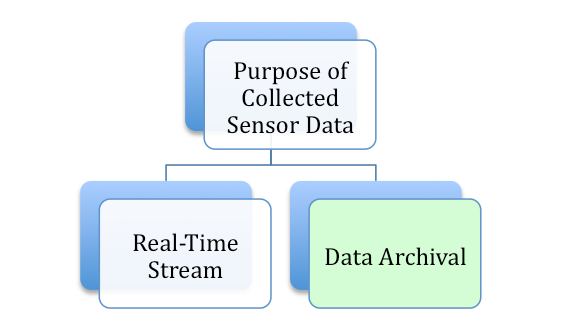
\includegraphics{../diagrams/taxonomy-data-purpose}
  \caption{The Purpose of Sensor Data Taxonomy}
  \label{fig:taxonomy-data-purpose}
\end{figure}

\begin{itemize}
  \item \textbf{Real-time Data Stream}: the collected data is accessed
  on-the-fly from the sensor device as a real-time data stream, and may have a
  short life cycle as it temporarily resides in memory;
  \item \textbf{Data Archival}: the collected data is used for historical
  purposes and is related to the historical data analysis \cite{sn-intro01,
  sn-intro02} or Information Fusion \ref{sn-info-fusion}. 
\end{itemize}

\section{The Location of the Sensor Data Taxonomy}

The location where the collected data is stored plays an important role
in the different aspects of the access to the collected data from sensor
devices, as shown in section \ref{sec:sn-storage-locations}. In this way,
Figure \ref{fig:taxonomy-data-location} depicts this taxonomy, which can be
described as follows:

\begin{figure}[h]
  \centering
  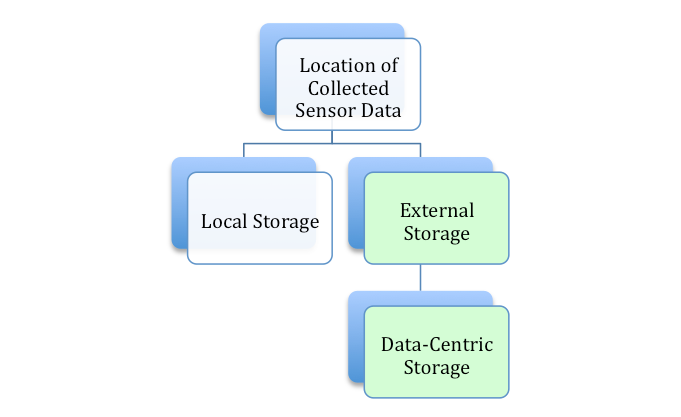
\includegraphics{../diagrams/taxonomy-data-location}
  \caption{The Location of Sensor Data Taxonomy}
  \label{fig:taxonomy-data-location}
\end{figure}

\begin{itemize}
  \item \textbf{Local Storage}: characterizes the placed of the collected data
  temporarily located in-memory, or in a secondary storage device on a node
  located in-network;
  \item \textbf{External Storage}: The collected data is usually located in an
  external storage device with a data management system such as a relational
  database;
  \item \textbf{Data-Centric Storage}: when the collected data occupies
  different external storages, being organized by categories based on the
  collected data keys and values. In other words, what characterizes this taxon
  is the presence of a data partitioning strategy to store the collected data.
\end{itemize}

\section{Data Model Taxonomy}

One of the fundamental challenges in the development of a persistence storage
in sensor networks is related to the data model chosen to represent the
collected data. Different data models were reported in the review of related
literature in section \ref{sec:data-models}. As a consequence, this taxonomy
relates to the data model used to design the collected data, as drawn in Figure
\ref{fig:taxonomy-data-model}, and described as follows.

\begin{figure}[h]
  \centering
  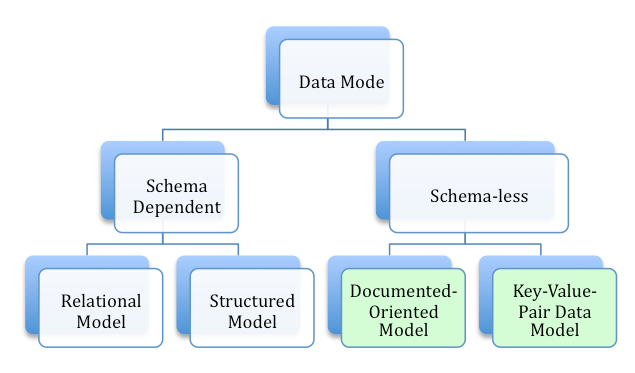
\includegraphics{../diagrams/taxonomy-data-model}
  \caption{Data Model Taxonomy}
  \label{fig:taxonomy-data-model}
\end{figure}

\begin{itemize}
  \item \textbf{Schema-Dependent Models}: this data model requires the
  definition of a master schema that describes the data through a rigorous of 
  data modeling process prior to the insertion of the data. Examples of such
  model is the traditional Relational Data Model\cite{relational-model}, as
 well as the Structured Data Models such as the XML \cite{xml};
  \item \textbf{Schema-less Models}: contrary to the former taxon, schema-less
  data models do not require the definition of a data schema or table
  definition. Instances of such data model reviewed in the literature review
  is the use of the Tabular Data model.
\end{itemize}

\section{Data Provenance Taxonomy}

No matter which data model used to represent the collected data, Data
Provenance provides a valuable guideline on how to describe the collected data
from sensors devices. As reported in section \ref{sec:sn-provenance}, the
description of the properties should take into account different properties of
the nature of the data as shown in Figure \ref{fig:taxonomy-data-provenance}.
Those taxa are summarized as follows:

\begin{figure}[h]
  \centering
  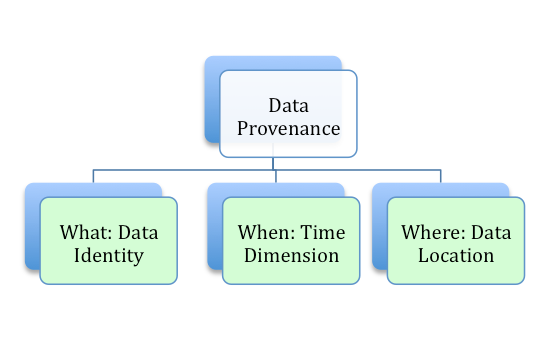
\includegraphics{../diagrams/taxonomy-data-provenance}
  \caption{Data Provenance Taxonomy}
  \label{fig:taxonomy-data-provenance}
\end{figure}

\begin{itemize}
  \item \textbf{What: Data Identity}: the data type that uniquely identifies
  the collected data from sensors. First and foremost, the properties of the
  sensor devices must be described according to the meaningful naming
  convention for the property. For instance, ``Water Temperature'' better
  describes the intent of the property as ``temp''. Second, the identification
  of the collected data related to the sensor type should be given, that is,
  which sensor device created the collected data, in case the data origin is
  relevant;
  \item \textbf{When: Time Dimension}: time is an important attribute of the
  data because it identifies the age of the collected data. Depending on the 
  use of the collected data, this is often taken into account. Two different
  types of time dimensions were described: \textbf{fact} and
  \textbf{transaction} times. The former is used to identify when the data
  was collected, whereas the latter when the data was transmitted to the
  data sink where the query processing acts;
  \item \textbf{Where: Data Location}: the point where the collected data was
  observed by the sensor device. Usually the latitude and longitude as the GPS
  coordinates are provided by devices which are capable of sensing the
  location. A descriptive metadata about the location could also be given such
  as room-name = ``deep see''.
\end{itemize}

\section{Query Processing Mechanism Taxonomy}

The query processing mechanism in sensor networks is directly related to how
and where the collected data is used and stored, as shown in section
\ref{sec:query-process}. As a consequence, the following taxa are related to the
different types of query processing mechanisms and summarized in Figure
\ref{fig:taxonomy-query-mechanism}:

\begin{figure}[h]
  \centering
  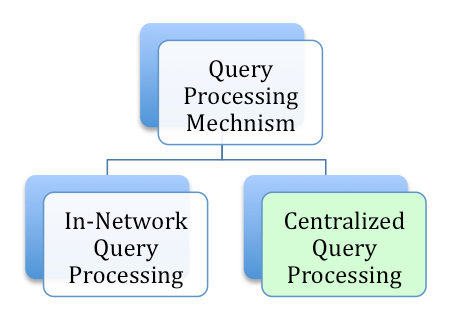
\includegraphics{../diagrams/taxonomy-query-mechanism}
  \caption{Query Processing Mechanism Taxonomy}
  \label{fig:taxonomy-query-mechanism}
\end{figure}

\begin{itemize}
  \item \textbf{In-Network Query Processing}: when the data node is the
  sensor device itself, and it uses the local storage mechanism, then the
  sensor node is able to reply to request related to the observations of the 
  environment defined by the sensor device. In this way, the query takes 
  place in the network itself, and usually returns values related to the current
  state of the environment;
  \item \textbf{Centralized Query Processing}: as developed by a single 
  relational database server, the data queried from a centralized data
  network sink in order to be reused. In general, this approach is used when
  the purpose of data is archival data.
\end{itemize}

\section{Database System Organization Taxonomy}

Different approaches of data systems were described in the literature review in
the last chapter in different sections. This taxonomy is directly related to
the use of external storage devices on a centralized network node so that it
often uses a single database server. Paradoxically, the use of a data-centric
storage determines the use of distributed database nodes around the network. 
In this way, Figure \ref{fig:taxonomy-database-architecture} describes the
taxonomy of the database system organization as follows:

\begin{figure}[h]
  \centering
  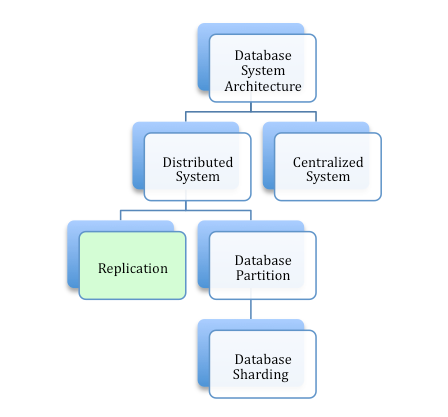
\includegraphics{../diagrams/taxonomy-database-architecture}
  \caption{Database Architecture Taxonomy}
  \label{fig:taxonomy-database-architecture}
\end{figure}

\begin{itemize}
  \item \textbf{Centralized System}: a database system that runs in one single
  centralized host, being the focal purpose of data traffic as read and writes 
  \cite{sn-intro01};
  \item \textbf{Distributed System}: a database system that can be composed by
  more than one node. Usually, the use of the pattern of Master-Slave
  mechanism or data ``Replication" is used. Another mechanism is the use of
  database paritioning, if the technology supports it.
\end{itemize}

\section{Relationships among the Taxonomies}

The different taxonomies defined in the previous sections of this chapter are
important to the understanding of a data persistence layer for sensor
networks. As they are closely related to each other, it is important to
briefly highlight these relationships in order to better analyze a problem
related to data persistence. 

The taxonomy related to the purpose of the sensor data can be directly related
to the taxonomy of the location of the sensor data. While the taxon of the 
real-time data stream relates to the local data storage, the taxon related to
data archival correlates the storage of the collected data into an external
storage. In addition to that, the converse is also true.

The taxonomy related to the data model can be related to any taxon from the
taxonomy of the location of the sensor data, as well as the taxons related to
Data Provenance. In the former, the data of a relational model is stored using
SQL messages.

In the light of these taxonomies, the classification of the data persistence
properties of a sensor networks can be studied and reviewed. As described in
the introduction of this dissertation, one the main motivations for this work
was to provide means of data persistence of NetBEAMS, a case study which does
not contain a data layer. Therefore, the following chapter seeks to describe
that case study in order to make a section of a given technology for evaluation.

% main.tex, to be used with thesis.tex
% This contains the main work of your thesis.

%\bibliography{thesis}  % uses the references stored in Chapter1Radar.bib

\chapter{Data Persistence for Sensor Networks: A Case Study for NetBEAMS}
\label{chap:netbeams-overview}

As discussed in Chapter 2, different properties of a sensor network and the
nature of the collected data must be taken into account in order to provide a
data persistence layer for a given sensor network. Similarly, in order to
better assist one's analysis of such functionality, Chapter 3 proposed a set of
data persistence taxonomies related to different properties of the collected
data life cycle. The goal of this chapter is to describe the fundamental properties 
of the case study used for this work, that is, NetBEAMS, in order to lay the 
groundwork as it relates to the selection of the database technology. NetBEAMS 
provides an automated infrastructure solution for SF-BEAMS, and this last component 
will be covered first. Then, this work proposes a categorization of NetBEAMS to 
the face of the taxonomies.

\section{SF-BEAMS: a Marine Sensor Network for Water Quality Monitoring}

As described by \cite{netbeams2009}, NetBEAMS is a joint venture between the
department of Biology and Computer Science at San Francisco State University,
whose goal is to automate the operational execution of SF-BEAMS. The San Francisco
Bay Environmental Assessment and Monitoring Station, or SFBEAMS \cite{sfbeams2006}, 
is an environmental sensor network system whose primary focus is the study of complex 
marine and estuarine environments using the SF-BEAMS sensors. The sensors are deployed off a
pier located on the San Francisco Bay, in Tiburon, California; and is operated by 
the Romberg Tiburon Center for Environmental Studies (RTC) a part of San Francisco
State University. NetBEAMS is an experimental component that utilizes the SF-BEAMS 
infrastructure to operate. This section details SF-BEAMS in general, and
presents the requirements for data persistence after classifying NetBEAMS based
on the taxonomies defined in the previous chapter.

\subsection{The SF-BEAMS Infrastructure}
\label{sec:sfbeams}

The SF-BEAMS sensor network is responsible for providing data for water quality
monitoring, as well as weather and surface conditions. Figure
\ref{fig:sf-beams} shows a picture taken from the SF-BEAMS web-camera.

\begin{figure}[!t]
  \centering
    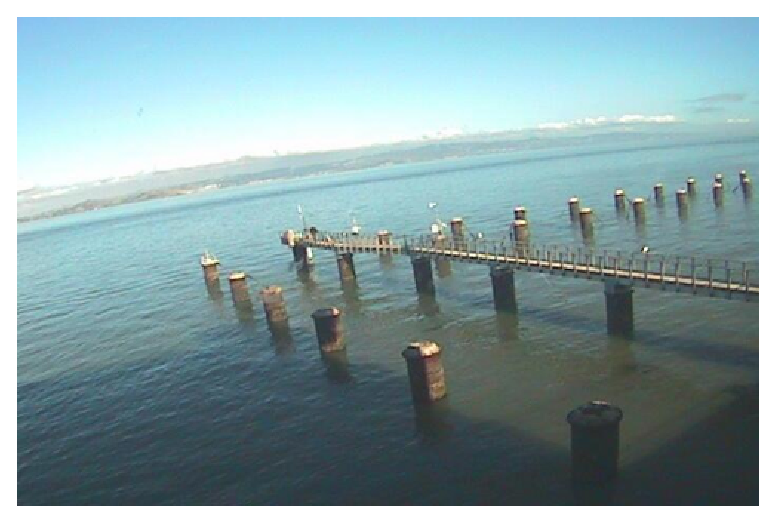
\includegraphics[scale=0.7]{../diagrams/cam_image-oct15}
  \caption{Picture of the SF-BEAMS Network, at the RTC pier. Tiburon, CA.}
  \label{fig:sf-beams}
\end{figure}

In general, the SF-BEAMS network infrastructure contains a varying number of
wired and wireless devices attached to pylons at the pier. Each of them
is responsible for observing different conditions of the area, having its own
mechanisms for internal storage for the collected data. In this way, data can
be directly transferred to the labs via Ethernet cables or collected manually
with a laptop computer. The current data collection process for SF-BEAMS is
described in Figure
\ref{fig:SF-BEAMS-system-architecture}\cite{sfbeams-current-system}. Upon
collecting data from sensors, the RTC staff uses automation scripts written in
Matlab \cite{matlab} to process, index and distribute the raw data in
different formats. One of these formats is the OPeNDAP \cite{opendap}, which
is widely used at research institutions to promote easier data exchange
amongst them. The SF-BEAMS website provides access to the collected data through
the Internet at http://sfbeams.sfsu.edu:8080/opendap. An example of an HTTP
Request from accessing the data for a specific YSI \cite{YSI-Sonde} is shown in
Listing \ref{file:rtc-ysi-opendap}.

\begin{figure}[!b]
  \centering
  \includegraphics[scale=0.5]{../diagrams/SF-BEAMS-system-architecture}
  \caption{The Current SF-BEAMS Data Collection Process}
  \label{fig:SF-BEAMS-system-architecture}
\end{figure}

As described in section \ref{sec:sn-infrastructure}, sensor devices produce
the observed data based on properties of measurements defined by its
manufacturer. NetBEAMS has used ``YSI 6600 ESD V2" \cite{YSI-Sonde}, as seen
in Figure \ref{fig:ysi-device}, one of the sensors devices used by SF-BEAMS.
It is a powerful water quality-monitoring device, capable of producing around
52 bytes on a single real-time data stream reading, as shown on Table
\ref{tab:ysi-data-stream}.

\begin{figure}[!b]
  \centering
  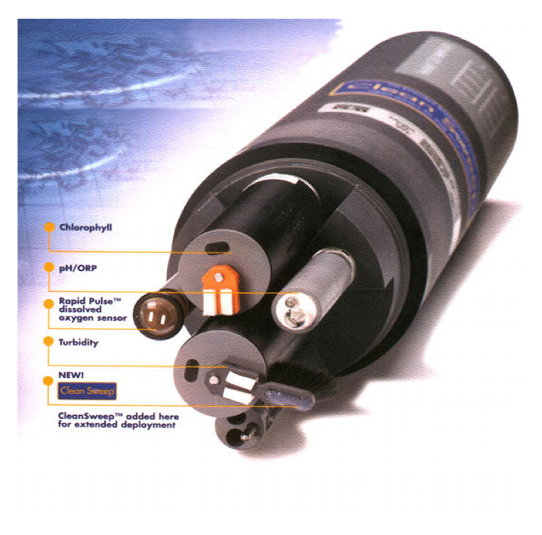
\includegraphics[scale=0.7]{../diagrams/ysi-device}
  \caption{Picture of the case study Sonde device: YSI 6600 ESD V2}
  \label{fig:ysi-device}
\end{figure}

\begin{table}
    \begin{center}
        \begin{tabular}{|l|}\hline
  12.20    192    179 5588.40   0.09   0.084   0.059  7.98   -79.6   99.5  8.83  0.4     8.7\\\hline
        \end{tabular}
    \end{center}
    \label{tab:ysi-data-stream}
    \caption{The Collected Data Stream from the YSI Sonde 6600ESDV2}
\end{table}

In order to have access to the observed data, the network staff downloads the
data using one of the device's connections such as the RS-232 serial connector
\cite{rs232}. Then, they upload the data into their data servers where they are
processed and archived for historical analysis. According to one
staff member, the infrastructure of the SF-BEAMS is comprised of the 
following components (as of May 2009):

\begin{itemize}
  \item 5 YSI Sonde devices, among others, in operation at the RTC pier;
  \item The sampling frequency rate is configured in ranges of either 1, 6 or
  15 minutes, depending on the specification;
  \item The processed data, used for distribution over the Internet,
   contains information regarding the time of the data collection.
\end{itemize}

Considering the infrastructure, the data load in the server-side
of RTC's laboratories produced by the YSI Sonde sensors devices can be
estimated by analyzing the data distribution over a period of one year, as
shown in Table \ref{tab:ysi-data-distribution}:

\begin{table}[!b]
    \label{tab:ysi-data-distribution}
     \begin{center}
      \begin{tabular}{|c|c|c|c|c|c|c|}\hline 
        \textbf{YSIs} & \textbf{Rate} & \textbf{Hourly} & \textbf{Daily} &
        \textbf{Weekly} & \textbf{Monthly} & \textbf{Yearly}\\\hline 
        1 & 1 min & 3.04 Kb & 73.12 Kb & 511.87 Kb & 1.99 Mb & 23.99 Mb\\\hline 
        5 & 6 min & 15.23 Kb & 365.62 Kb & 2.5 Mb & 9.99 Mb & 119.97 Mb\\\hline 
        1 & 15 min & 0.5 Kb & 12.18 Kb & 85.31 Kb & 341.25 Kb & 3.99 Mb\\\hline 
        5 & 1 min & 2.54 Kb & 60.93 Kb & 426.56 Kb & 1.67 Mb & 19.99 Mb\\\hline
        1 & 6 min & 0.2 Kb & 4.87 Kb & 34.12 Kb & 136.5 Kb & 1.6 Mb\\\hline 
        5 & 15 min & 1.0 Kb & 24.37 Kb & 170.62 Kb & 682.5 Kb & 7.99 Mb\\\hline
        \end{tabular}
      \end{center}
    \caption{Amount of data produced by the RTC's YSI sondes}
\end{table}

The maximum amount of data produced by the YSI Sonde device is hundreds of Megabytes
a year, as \textbf{483,840} samples are generated by one single device. 

\subsection{Taxonomic Classification of SF-BEAMS}

This section classifies the sensor network deployed by SF-BEAMS according to
the taxonomies proposed in the previous chapter. This classification is
necessary to better understand the requirements of a data persistence for
NetBEAMS, which indirectly uses the infrastructure of SF-BEAMS.

\begin{itemize}
  \item \textbf{The Purpose of Sensor Data}: the data from SF-BEAMS is exclusively
  used for the purpose of Data Archival, since they are stored in RTC's lab;
  \item \textbf{The Location of the Sensor Data}: it is clear that the purpose
  of the data is directly related to the sensors location and, thus, the
  strategy of \textbf{External Data Storage} is used to store its collected
  data at the network sink at the RTC site;
  \item \textbf{Data Model}: since the format used by the RTC staff to share
  data with researchers is in the OPeNDAP format, the data
  model used is the tabular data model, since it uses the comma-delimited
  files. In this way, the \textbf{Schema-less} model is used;
  \item \textbf{Data Description}: once the collected data reaches the RTC
  lab, a quality assurance process is executed, and the data is transformed
  into the format used by OPeNDAP. This conversion carries data regarding
  the time of the data collection, therefore, one of the
  \textbf{Time Dimensions} such as the valid time is used. Since the files are stored
  with specific file name structure, using timestamps to describe the data, the
  use of transaction time may be also considered. Finally, the contents of the
  files contain the \textbf{Data Identity} as shown in the samples of
  the collected in Listing \ref{file:rtc-ysi-opendap};
  \item \textbf{Query Processing Mechanism}: similar to the data stored in a
  centralized way, the query processing is also \textbf{Centralized}, as the
  data is stored on file system;
  \item \textbf{Data Volume}: the volume of data produced is characterized by small.
 It is related to the volume of data produced by the sensor devices,
  which is numerical data streams, and the total number of sensor devices;
  \item \textbf{System Organization}: SF-BEAMS runs on a Single System, as
  the collected data is stored directly in the file-system after previous 
  processing. However, the collected data is provided to the Internet using
  the OPeNDAP Hyrax system as a middleware.
\end{itemize}

\section{NetBEAMS: a component-based approach for SF-BEAMS}
\label{sec:problem-requirements}

Although the execution of RTC's sensor network can be operated as it
was mentioned in the previous sections, \cite{netbeams2009} described some of the
operational challenges faced by the RTC staff during regular activities of the
data collection process. It was clear to the research group that SF-BEAMS
could have not only its data gathering process automated, but also its data
management and distribution. By the use of COTS\footnote{Common-Off-The-Shelf
designates a product that is produced and sold in bulk} embedded devices and
open-source \cite{open-source} software, the research group developed a second
version of NetBEAMS, a component-based approach which suggested the improvement of 
operational activities from SF-BEAMS using systems automation. In brief, one of the 
ongoing problems of NetBEAMS was regarding Data Persistence, the primary motivation of
this report.

The Networked Bay Environmental Assessment and Monitoring System, or Net-BEAMS,
offers the Data Sensor Platform (DSP) \cite{netbeams2009} as the system
architecture that can address the operation of SF-BEAMS. The in-depth
documentation describing the DSP Platform, including its architecture and data
gathering process is provided at the online documentation 
\cite{netbeams-dsp-architecture}.

The scope of this work is defined as to provide a persistence layer for
NetBEAMS, making a selection of a persistence layer that is an exception to the
taxonomical classification of SF-BEAMS. Furthermore, the technology to be
selected for the persistence layer must take into account the requirements of
NetBEAMS primary users such as Computer Science researchers, as well as end
users such as Biologists from the RTC laboratories. The requirements for the
data persistence specifically for NetBEAMS are described in the following
section.

\section{Requirements for NetBEAMS Data Use}

The main reason for the operation of SF-BEAMS using NetBEAMS's automated
approach is that it can potentially reduce operational costs and improve the
data collection process. In view of this, the scope of a persistence layer
can be summarized as a group of functional and non-functional requirements in
order to select a database system for the sensor network supported by NetBEAMS.

\subsection{Functional Requirements}

\begin{itemize}
  \item Reuse the NetBEAMS infrastructure and develop a component responsible
  for data persistence in a database system;
  \item The Persistence System must obey to the characteristics of the
  categorization of SF-BEAMS used by the taxonomies.
\end{itemize}

\subsection{Non-Functional Requirements}

\begin{itemize}
  \item The data model used to describe the data must not impose restrictions
  to the users of the system (i.e. Biologists and students without expertise in
  Database Systems);
  \item Data Representation must be similar to those used by RTC, with a
  more human-readable format;
  \item The system must be scalable with a low degree of maintenance, in a
  way that the interruptions to the data gathering process are infrequent;
  \item Data must be searchable in near-real-time with good performance;
  \item The system must also support export capabilities, which may
  be used to match RCT's requirements of the OPeNDAP format;
  \item The database must be free of charge, following the
  implementation specifications of NetBEAMS for Open-source software.
\end{itemize}

In conclusion, after detailing the SF-BEAMS sensor network, and describing the 
infrastructure of NetBEAMS, its the motivation and goals for this project were 
presented. The next chapter is the actual analysis of existing database systems 
mentioned in Chapter 2, which aligns with the requirements and characteristics of 
NetBEAMS. Meanwhile, more details regarding the architecture of NetBEAMS, as well as
the development guidelines can be found in the appendix of chapter 10.

% main.tex, to be used with thesis.tex
% This contains the main work of your thesis.

%\bibliography{thesis}  % uses the references stored in Chapter1Radar.bib
\setcounter{table}{1}
\chapter{Empirical Analysis of Data Persistence Taxonomies for NetBEAMS}

Providing data persistence for an existing sensor network requires analysis of
the infrastructure and the nature of the data produced. Based on the
taxonomies of Chapter 3, and the requirements of a data persistence for
NetBEAMS in Chapter 4, this chapter aims at analyzing a group of database
technologies selected from the topics covered in Chapter 2.
Similarly, supported by the scope of the required implementation presented in
this chapter, the comparison of the technologies is summarized, highlighting
the selected database system used for the design of a component for NetBEAMS
and used for the design of the experiments.

\section{Scope of the use of the Technology}

The scope of the use of the database can involve different functional and
non-functional requirements defined in the last chapter. This work does not
intend to implement an application based on the database system selected, but
to provide the foundation of a database management system that can be used to
develop one focused less in refactoring and high scalability and performance.
For this reason, the use of the database system will be restricted to the data
persistence and use through a native system or through the use of native
programming languages or API. In this way, the scope of this technology
selection can be summarized as follows:

\begin{itemize}
  \item Provide data management over the collected sensor data, as a
  conventional database systems;
  \item Must be able to scale in any increases to the data load of
  the sensor network, as described in Chapter 2;
  \item  Must be able to use single or multiple servers to improve performance
  and optionally deal with Data-Centric approaches to sensor data partitioning;
  \item Must provide a data model that scales, decreasing the constant data
  schema changes.
\end{itemize}

\section{Database System ``Contenders''}

This section describes the database systems ``contenders'' considered to be used
as the persistence technology backend for NetBEAMS. As described in the
previous chapter, the selection of the technologies must be based on the list
of functional and non-functional requirements specified within the scope of
this work.

One of the essential questions related to data persistence is regarding the
data model and types of the database. That is, the use of the relational or
any other model to describe data along with its management. Traditionally, the
relational data model has been used to provide data persistence for different
types of projects, including sensor networks \cite{sn-dataware-house,
db-xml-enabled, sn-db-tinydb}. However, tradition does not always get
translated into efficiency in terms of problem solving. For this reason,
\cite{db-is-rdbs-dommed} reflects about the use of alternatives to the
relational model when the data persistence problem in consideration is to
provide data persistence for dynamic environments such as Internet applications.
The author also suggests that the relational model is hard to maintain in
ever-changing environments, and thus, proposes the use of the Key-Value-Pair
(KVP) data model and a different number of technologies. Similarly,
\cite{cloud-comp-survey} reports similar trends in academic and industrial
research in distributed computing using KVP databases in powerful systems
such as Cloud Computing \cite{cloud-comp-architectures}. For this reason, in
addition to the different database systems used by projects in the
literature review, this work also includes the review of a KVP database system
called mongoDB \cite{mongodb}, since it was among those cited in the surveys.
In such a manner, the list of the systems considered for assessment is the
following:

\begin{itemize}
  \item \textbf{MySQL}\cite{mysql}: an open-source relational database
  system popularized by the development of Internet applications, maintained
  by Sun Microsystems. \cite{sn-dataware-house} reports its use to develop a
  data warehouse for data collected from sensor devices using this technology;
  \item \textbf{TinyDB}\cite{tinydb}: developed and maintained by the Computer
  Science department of University of California, Berkeley, TinyDB is a
  relational database system specially developed for sensor devices. As
  referred in Section \ref{sec:sn-persitence-storage}, it is system used in
  many different sensor networks implementation such as \cite{sn-db-tinydb,
  sn-db-newop};
  \item \textbf{MongoDB}\cite{mongodb}: an open-source KVP database
  system suggested by different surveys to be an alternative to relational
  databases \cite{db-is-rdbs-dommed, cloud-comp-architectures}. It is maintained
  by 10Gen Incorporated;
  \item \textbf{DB2}\cite{db2}: in the pursuit of an XML database system, DB2
  is listed as a hybrid database system that offers both the relational and the
  XML models \cite{db-xml-enabled}. It is privately owned by IBM.
\end{itemize}

The following sections review these technologies' capabilities to adhere to
the specifications of the taxonomies defined in Chapter 3, as well as the
requirements and the scope for a data persistence of NetBEAMS, as defined in
Chapter 4.

\section{Analysis of the Purpose of Sensor Data}

The execution of the SF-BEAMS sensor network, together with the NetBEAMS
automated infrastructure, can be summarized as follows:

\begin{itemize}
  \item Data is generated by sensor devices, such as the YSI Sonde
  \cite{YSI-Sonde}, and manually collected by using a laptop to the data sink
  at the RTC laboratories;
  \item Upon data reception, the RTC staff index and archive the data for
  distribution using the OPeNDAP format;
  \item An automated approach to the data collection procedures is performed 
  using NetBEAMS \cite{netbeams2009}, using software components to obtain and
  send the data to the data sink node. A complete description of this approach
  is \cite{netbeams-dsp-architecture}.
\end{itemize}

The nature of data from NetBEAMS through SF-BEAMS is used for the purpose of
\textbf{Data Archival}. After the collected data captured from the sensors, it
requires further processing in order to be archived for later reuse. Different
types of users are expected to use the collected data, ranging from
researchers, students, and the public over the Internet.

\subsection{Technology Analysis}

Since all of developed database systems were implemented with the intention of
persisting data in long-term storage devices, every one listed provides
support for data persistence and management. Therefore, they are compliant to
the purpose of Data Archival for the sensor networks.

\section{Analysis of the Location of Sensor Data}
\label{sec:sn-data-location}

The advantages of the External Storage approach is the most common way to
implement persistence for any type of systems since data management is usually
offered by most database systems out-of-the-box. It is basically used to store
small volumes of data. On the other hand, the most common problems related to a
single External Data Storage approach are related to the capacity of the
device and operational problems. If the external storage device is situated in
the network, then the capacity of the device may be limited to receive
collected data from the sensors in the network, since it may run out of space.
Similarly, storage devices are very error prone and its hardware part may fail.

As shown in the previous chapter, NetBEAMS's architecture is based on sensor
network whose topology is a single-hop star with a centralized data sink. In
this way, all the collected data is transmitted to that single location as
described in Section \ref{sec:sn-infrastructure}. The simplest location to save
the collected data is through the use of at least an \textbf{External
Storage}. Similarly, the use of a Data-Centric Storage strategy is considered
in situations where the data sink is about to reach its storage capacity. The
\textbf{Data-Centric Storage} separates the collected data into dissimilar
locations, based on any property of the data. Therefore,
there are two different approaches to data partitioning:

\begin{itemize}
  \item \textbf{Horizontal Partitioning}: the data segmentation is implemented
  based on the values of the table rows, in the relational model point of view,
  or the collections elements, on KVP databases. That is, all the values defined
  by the columns are used in a given table physically located in specific
  servers. For instance, horizontal partitioning can be defined as a
  collection of five years worth of historical sensor data, partitioned into
  five separate servers. In this way, each server contains data related to
  each of the years;
  \item \textbf{Vertical Partitioning}: data is partitioned vertically in a way
  that the columns of an entity on the relational model are divided into
  different database tables. In this way, the particular dataset is broken
  down to different tables. For example, if the database is used to store
  pictures of a given sensor camera in a BLOB column, it would be the most
  preferable to the scenario where the images are not constantly referenced
  when compared to the textual data. Since KVP uses denormalized data, this
  partitioning strategy is not used.
\end{itemize}

\subsection{Advantages of the Data-Centric Approach}

The benefit of the Data-Centric approach can be directly associated with
database partitioning mechanisms described earlier. Since the collected data is
distributed into different locations, this approach decreases the size of
datasets when the database server performs a query processing in a database
table. For this reason, this approach helps the database administrators scale
their database infrastructure and improve the database performance.

The horizontal or vertical partitioning strategies are also referred to as
Database Sharding \cite{db-shard-discussion}, or simply Database partitioning
\cite{db-partitioning-relational}. Both the former and the latter are used in
regular schema-dependent models or schema-less models. Different approaches
worth mentioning:

\begin{itemize}
  \item \textbf{Hash Partitioning}: a hash key is computed based on
  different table columns of an entity \cite{db-shard-schemas,
  db-partitioning-relational}, providing an even distribution of the data;
  \item \textbf{Key Partitioning}: is based on the hash partitioning over the
  values of a specific key \cite{db-mongo-partition};
  \item \textbf{Range Partitioning}: the partition is based on specific ranges
  of the values of given a given column of a table. For instance, the collected
  data from the sensors could be separated by the year of its collection. For
  example, data collected in the year of 2009 would be stored in a different
  partition than the data collected in the year 2010
  \cite{db-partitioning-relational}.
\end{itemize}

An example of a data-centric storage with different partitions can be seen in
Figure \ref{fig:database-sharding-by-region}, where the collected data is
partitioned by its origin. Each shard is assumed to be placed in different
server hosts, as well as each of them uses the same ``denormalized'' data
models.

\begin{figure}[!h]
  \centering
  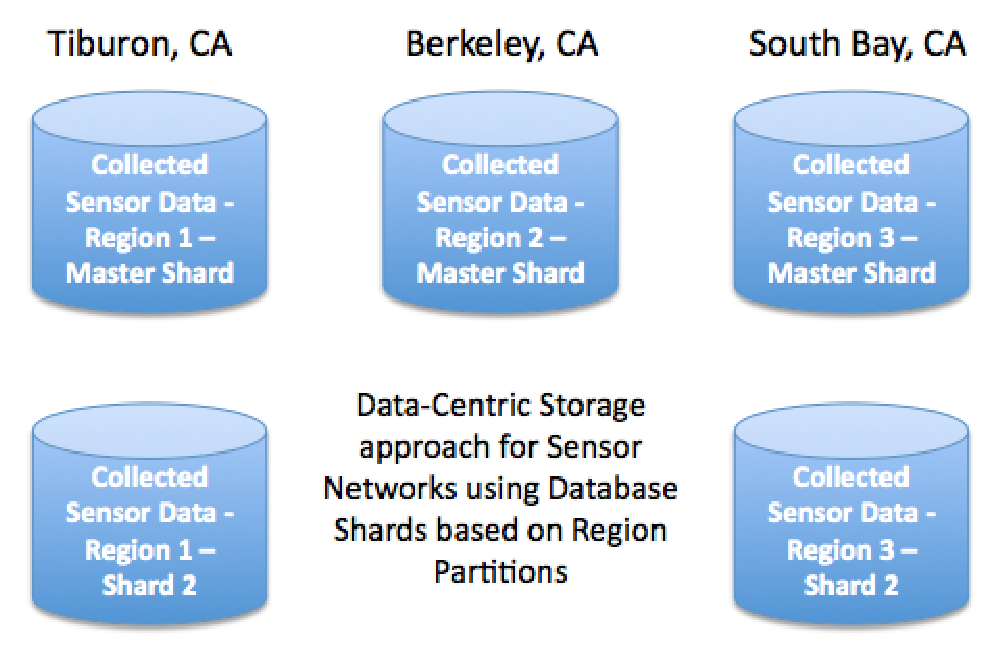
\includegraphics[scale=0.5]{../diagrams/database-sharding-by-region}
  \caption{Example of Data-Centric Storage for Sensor Networks using Database
  Sharding}
  \label{fig:database-sharding-by-region}
\end{figure}

\subsection{Disadvantages of the Data-Centric Approach}

The data partitioning is a highly restricted technology, normally available to
advanced users of distributed database systems. Despite being offered as a
common-off-the-shelf functionality by some popular database systems, this
strategy requires closer database management and configuration. Some of the
problems related to this strategy are regarding its lifecycle management
\cite{db-shard-discussion}:

\begin{itemize}
  \item \textbf{Rebalancing Partitions}: considering a schema-dependent database
  system, changes on the schema of one shard requires rebalancing the
  collected data on each of the shards. As a consequence, the database shards
  transfers data to new locations whenever necessary. This technique is
  starting to appear as COTS implementations such as MySQL \cite{mysql} and
  mongoDB \cite{mongodb};
  \item \textbf{Referential integrity}: also considering a schema-dependent
  database system, any cross-shard query may run into the problem where
  references do not exist in other shards, since the application layer is
  responsible for enforcing data integrity. In this way, examples of such
  include verifying constraints of foreign keys when the partition is done
  using Vertical table partitioning, considering that data collections are
  organized in separate spaces, and physically placed in different shard nodes
  \cite{db-partitioning-relational}.
\end{itemize}

\subsection{Technology Analysis}

\begin{itemize}
  \item \textbf{MySQL}: Supports External or Data-Centric Storage approaches.
  When Data-Centric Storage is used, both vertical and horizontal partitions
  \cite{db-partitioning-relational} can be chosen, using different strategies
  to partition the data;
  \item \textbf{TinyDB}: Only supports the External Storage;
  \item \textbf{MongoDB}: Supports External or Data-Centric Storage. When the
  latter approach is used, the horizontal partition strategy is available with
  automatic shards \cite{db-mongo-partition};
  \item \textbf{DB2}: Supports External and Data-Centric storage. Only supports
  vertical table partition for the data-centric storage \cite{db-db2-partition}.
\end{itemize}

All the selected database systems support the External Storage method. However,
they all differ somewhat in terms of Data-Centric Storage support. Therefore,
MySQL and mongoDB are promising choices, with the difference of the use of the data model.

\section{Analysis of the Data Model}

One of the most common practices in the area of database system is to use the
relational model for data persistence, although the application of the system
may not fit to solve the problem. In fact, the main users of sensor networks may
not possess any expertise in database systems or data modeling, based on the
fact that they are from different science areas. \cite{sn-programming-language}
suggested the use of programming languages abstraction, instead of regular
database systems, to provide access to the collected data for both
technical and non-technical users. For instance, marine biologists manage
SF-BEAMS without expertise in data management or modeling systems. For this
reason, one of the requirements of the system is the use of a schema-less
approach, which describes the collected data without data modeling process
used in schema-dependent models. The \textbf{Key-Value-Pair Data Model} seems
to be an optional candidate that provides such a method of data design.

\subsection{Analysis of the Schema-Dependent Models}

Considering the inception of a relational data model \cite{relational-model}
and the use of the YSI Sonde data as the main entity in the system, Figure
\ref{fig:Relational-Model-Original} represents a prototype of the relational 
model, after passing through the process of normalization
\cite{db-normalization}.

\begin{figure}[!t]
  \centering
  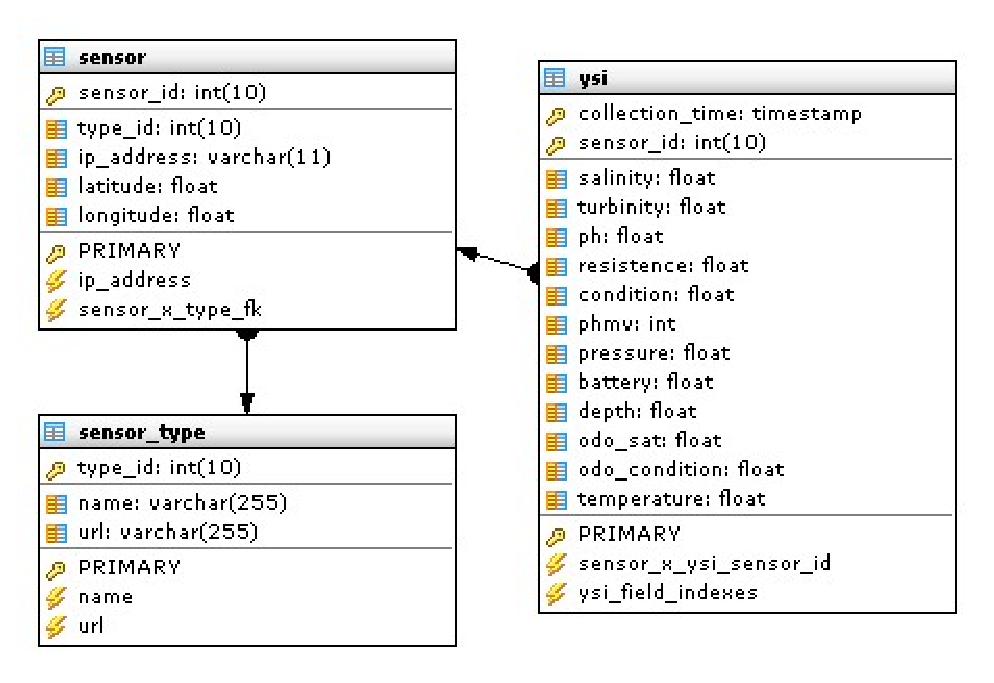
\includegraphics[scale=0.65]{../diagrams/Relational-Model-Original}
  \caption{Relational Data Model for NetBEAMS - A first prototype}
  \label{fig:Relational-Model-Original}
\end{figure}

When a new type is added into the system, the refactored version of the
relational model be depicted in Figure
\ref{fig:Relational-Model-Addition-Modified}. Some observations are considered
in this scenario:

\begin{figure}[!b]
  \centering
  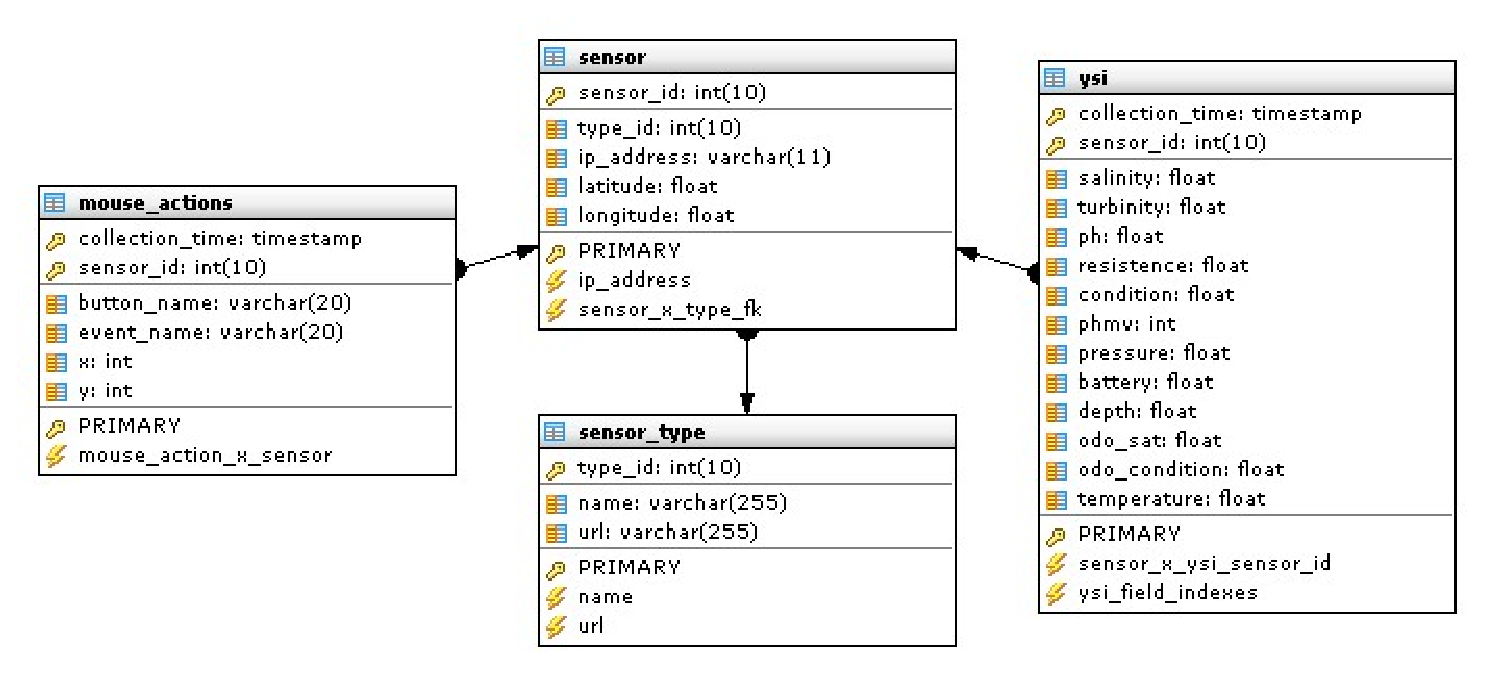
\includegraphics[scale=0.6]{../diagrams/Relational-Model-Addition-Modified}
  \caption{Relational Data Model for NetBEAMS - Modified version with new
  entity}
  \label{fig:Relational-Model-Addition-Modified}
\end{figure}

\begin{itemize}
  \item Data schema that constantly change requires continuous database
  normalization processes, changes to structure, database management, and all
  the code that uses the data. Schema-Dependent databases always require
  refactoring of the schema to accommodate changes to the entities' properties;
  \item \cite{sn-provenance} describes the relational model as problematic 
  when describing collected data from sensor devices;
  \item \cite{sn-db-newop} suggests changes to the SQL clauses of TinyDB to
  better support time-series, an important property when describing
  collected data from with spatial-temporal properties.
\end{itemize}

Other projects have used the XML data models for persistence. It falls
into the same category as the Relational Model using XML documents \cite{xml},
since XML documents must fulfill the specifications defined by an XML Schema
\cite{xml-schema}. This model uses XPath \cite{xml-xpath} technology for
querying documents, although some hybrid \cite{db2} technologies may still use
SQL \cite{sql} for that matter. In this way, the view of an example of database
state for the defined previous schema can be seen in Figure
\ref{fig:persistence-example-relational}.

\begin{figure}[!h]
  \centering
  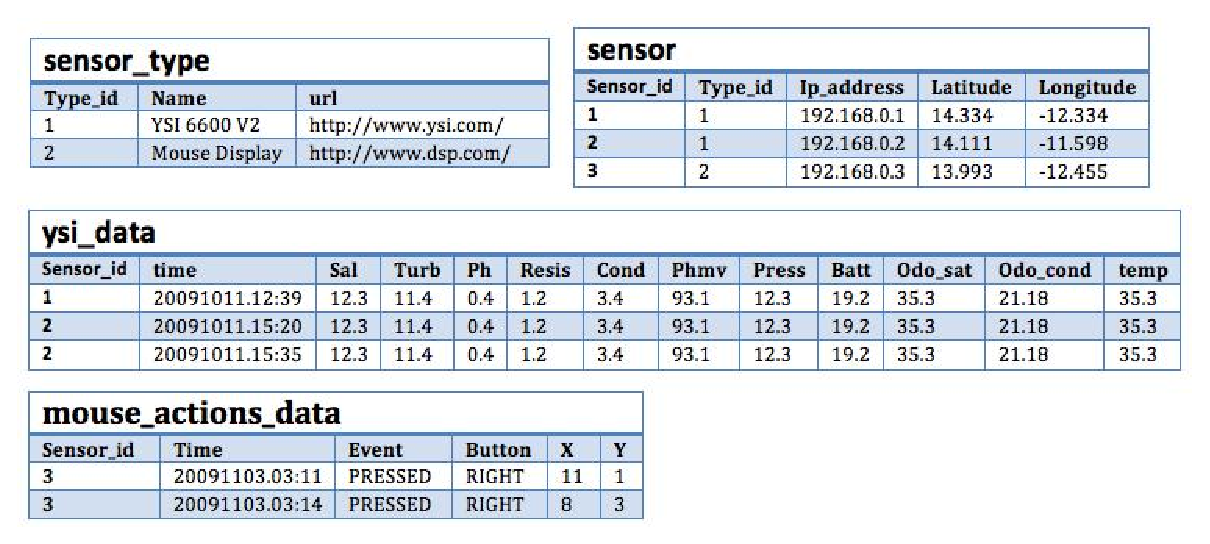
\includegraphics[scale=0.7]{../diagrams/persistence-example-relational}
  \caption{Instance of a Relational Model Database Prototype}
  \label{fig:persistence-example-relational}
\end{figure}

This data model has been used to solve data models for different types of
application. One such a problem is the one to represent entities by a list of
properties with keys and relating values, called Key-Value data model
\cite{db-kvp-in-relational01, db-kvp-in-relational02}. The author of
\cite{db-kvp-in-relational01} suggests that this is used as a technique used
when the addition of number of properties of an entity constantly changes, and
thus, requires constant refactoring of the relational data model. Considering
this data model for sensor network devices, whose properties are lists of keys
and relating values, an ``one-fits-all'' attempt to use the KVP data model
using the relational data model is depicted in Figure
\ref{fig:KVP-on-Relational-Model}, and a given example of the state of a
database using this schema in Figure
\ref{fig:persistence-example-relational-kvp}.

\begin{figure}[!h]
  \centering
  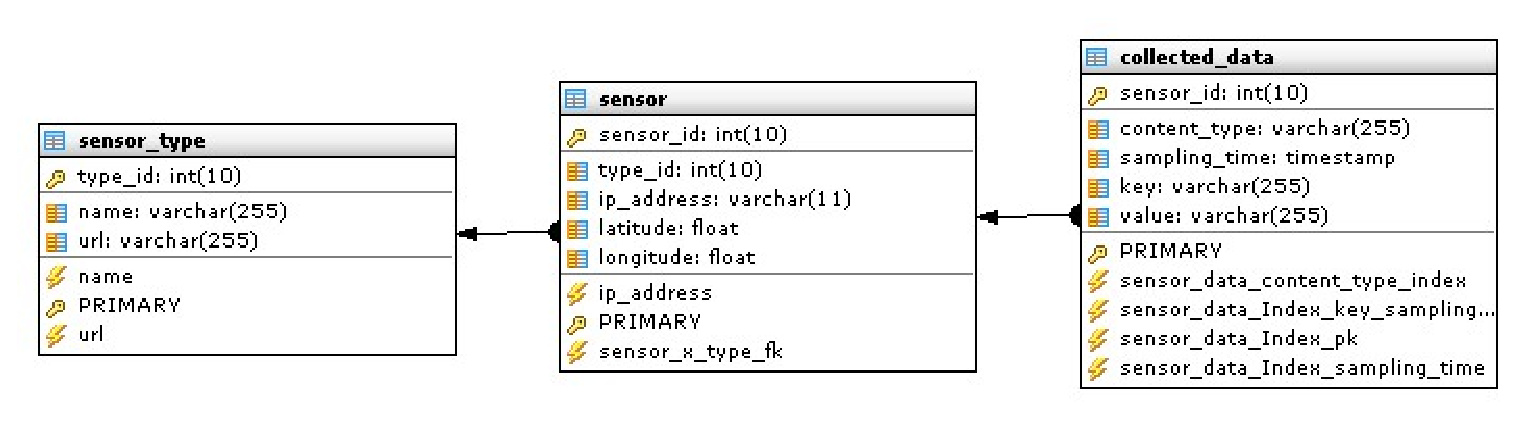
\includegraphics[scale=0.6]{../diagrams/KVP-on-Relational-Model}
  \caption{KVP Data Model implementation using Relational Model}
  \label{fig:KVP-on-Relational-Model}
\end{figure}

\begin{figure}[!h]
  \centering
  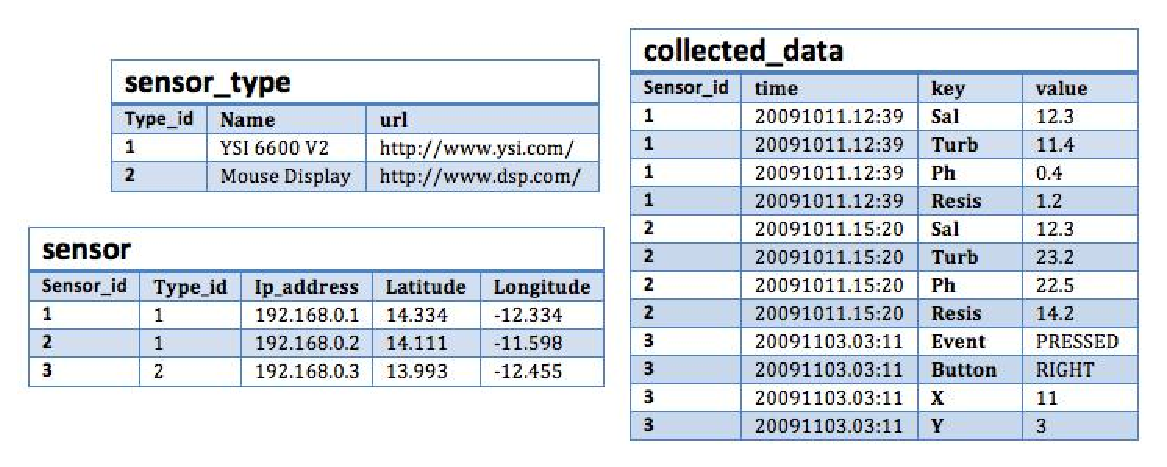
\includegraphics[scale=0.75]{../diagrams/persistence-example-relational-kvp}
  \caption{KVP over Relational Model Database Prototype}
  \label{fig:persistence-example-relational-kvp}
\end{figure}

\newpage

\subsection{Analysis of the Schema-less Models}

The growth of distributed systems and the Internet have enabled the development
of powerful database servers that can be organized in the context of
infrastructure and how to represent models. A powerful up-coming approach is
the use of database systems that do not use structured language for querying
its data. One such example is called Key-Value Pair (KVP) data model
\cite{db-kvp}, and it is characterized as follows:

\begin{itemize}
  \item data is structured in collections of key-value pairs, as it is done in
  hash data structure. The definition of the key is a given property with its
  associating value;
  \item the query process is using mechanics similar to programming or
  scripting language, that is, the use of APIs in a given programming language.
\end{itemize}

There are no records of the use of this data model with sensor networks. Data
is generally aggregated by given entities and any needed property applied to
it. Key may be composed by embedded keys having a dynamic structure and freely
used without a schema validation mechanism as used schema-dependent data
models, having the following organization:

\begin{itemize}
  \item entities from the same domains are placed into a ``bucket'';
  \item entities have a set of attributes and relating values;
  \item entities with different set of attributes may be contained in the same
  bucket, since there is no schema to govern the bucket items restriction.
\end{itemize}

For instance, all data needed for the YSI Sonde Data, as well as all necessary
provenance data and annotation as defined in Section
\ref{sec:sn-data-description}, are represented by means of key-value pairs as
seen in Figure \ref{fig:persistence-example-kvp}.

\begin{figure}[!h]
  \centering
  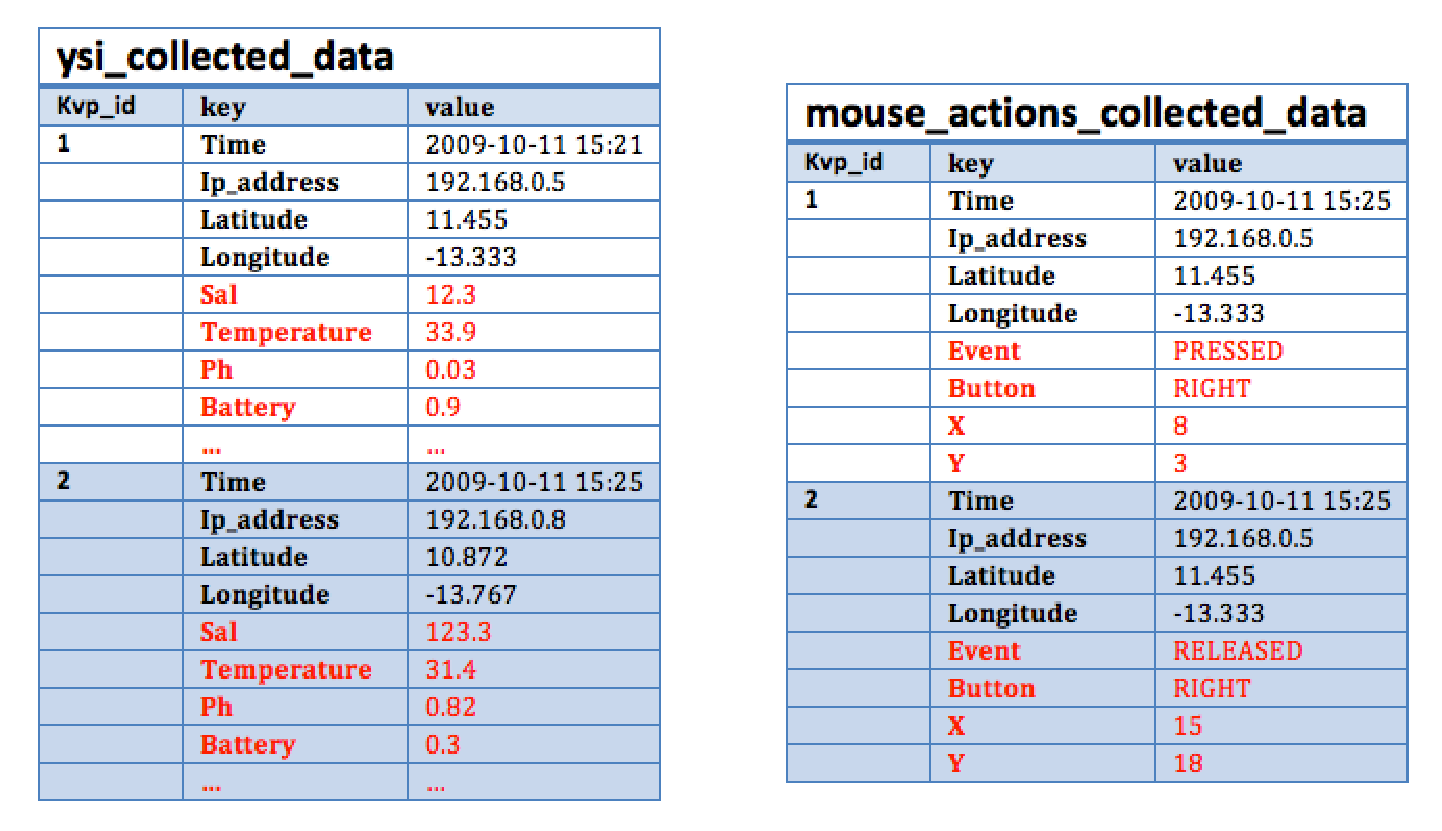
\includegraphics[scale=0.5]{../diagrams/persistence-example-kvp}
  \caption{KVP Database instance Prototype}
  \label{fig:persistence-example-kvp}
\end{figure}

\subsection{Technology Analysis}

The properties of the relational and key-value data models were compared by
\cite{db-is-rdbs-dommed} and summarized in Table 5.1:

\begin{table}[!b]
    \label{tab:properties-schema-vs-schemaless}
    \caption{Schema-Dependent X Schema-less Databases Compared: Properties}
    \begin{center}
    \begin{tabular}{|p{210pt}|p{210pt}|}\hline
    Schema-Dependent Databases & Schema-less Databases\\\hline
    \begin{enumerate}
      \item Real-world model represented by entities, classified in tables;
      \item Tables composed by columns and rows. Rows are comprised by column
      values, which have the same schema;
      \item Data Model is defined in advance with a schema, which contains
      relationships and constraints to enforce data integrity;
      \item Data represents ``natural'' entities, not application specific;
      \item Data Normalization is the data structuring process to remove data
      duplication, as well as establishing data associations through table
      relationships \cite{db-normalization};
      \item Data Provenance can be provided through data types such as
      ``timestamp'' for time or float for the GPS float-based coordinates; 
    \end{enumerate} 
    & 
    \begin{enumerate}
      \item Real-world model by entities, classified in Domains;
      \item Domains are similar to tables, but like buckets that contains items
      without a pre-defined schema, what enables them to have different schemas;
      \item Items are identified by keys, as well as have a dynamic set of
      attributes attached to it, however with no schema defined;
      \item Items may represent not only the natural representation of data, but
      also include application-specific data;
      \item Since data may be repeated, no data normalization is done, so that
      integrity is done in the application layer;
      \item Data provenance can be added through the use of keys and relating
      values for the time information and location of the data.
    \end{enumerate}
    \\\hline
    \end{tabular}
    \end{center}
\end{table}

\newpage

In order to have access to the persisted data, both types of data models
support methods: one via structured languages, and the other via abstractions
of programming languages. \cite{db-is-rdbs-dommed} summarizes the differences
shown in Table 5.2:

\begin{table}[!h]
    \label{tab:daccess-schema-vs-schemaless}
    \caption{Schema-Dependent X Schema-less Databases: Data Access}
    \begin{center}
    \begin{tabular}{|p{210pt}|p{210pt}|}\hline
    Schema-Dependent Databases & Schema-less Databases\\\hline
    \begin{enumerate}
      \item The basic CRUD (Create-Retrieve-Update-Delete)
      database operations are performed using a structured language such
      as the SQL or XPath;
      \item Query languages can access data from different tables through
      joins, containing aggregation functions to apply on the returned values.
    \end{enumerate} 
    & 
    \begin{enumerate}
      \item The CRUD operations are performed via an abstraction of
      programming language. (E.g. ``db.collection.find()'',
      ``db.collection.insert()'');
      \item Some technologies provide basic SQL-like syntax for filter criteria
      with some predicates like equals to (=), different than (!=), less than
      or equals ($\leq$), greater than or equals ($\geq$), among others;
      \item The data and application integrity logic is placed in the
      application layer.
    \end{enumerate}
    \\\hline
    \end{tabular}
    \end{center}
\end{table}

Finally, each data model provides its own APIs to the integration with external
systems. \cite{db-is-rdbs-dommed} differentiates each of the application interfaces
provided by each of them, as summarized on table 5.3.

\begin{table}[!h]
    \label{tab:api-interface-schema-vs-schemaless}
    \caption{Schema-Dependent X Schema-less Databases: Application Interface}
    \begin{center}
    \begin{tabular}{|p{210pt}|p{210pt}|}\hline
    Schema-Dependent Databases & Schema-less Databases\\\hline
    \begin{enumerate}
      \item Have their own specific API or through ODBC (Open Database
      Connectivity);
      \item Data is stored in a format that represents its natural structure,
      and for this reason, in a single or distributed fashion.
    \end{enumerate} 
    & 
    \begin{enumerate}
      \item Tend to provide Web Services Interfaces such as the REST
      \cite{http-rest};
      \item \cite{db-is-rdbs-dommed} claims that data is stored in a more
      effective way, requiring only code plumbing for the relational code;
    \end{enumerate}
    \\\hline
    \end{tabular}
    \end{center}
\end{table}

The data model used by each of the selected database systems can be summarized
as follows:

\begin{itemize}
  \item \textbf{MySQL}: uses the Relational Data Model with the use of SQL;
  \item \textbf{TinyDB}: uses the Relational Data Mode with the use of SQL; 
  \item \textbf{MongoDB}: uses Key-Value Pair Data Model with an abstraction of 
  programming language functions calls;
  \item \textbf{IBM DB2}: uses the Relational and Structured models with SQL
  and XPath, respectively.
\end{itemize}

\section{Analysis of the Data Description}

\textbf{Data Description} is the method used to describe the collected data
from sensors, especially those produced by real-time data streams. Since that
type of data does not include descriptions of its values, data provenance
offers guidelines to improve the description of the collected data.

In addition to data provenance, annotation is another technique used to
better describe the collected data from sensor devices. Its main purpose is to
provide a means of identifying observations, creating indexes based on simple
keywords. For an environmental sensor network, this is invaluable used to
better manage the collected data.

\subsection{Use of Provenance-Aware Data}

The inclusion of provenance data into the collected data enriches the
description of a given event, and is always useful to determine different
aspects of the data. As mentioned in Chapter 3, data provenance helps identify
the nature of the data by the identification of the properties of a given
sensor device, for example. Similarly, provenance adds spatial-time data in
order to correlate the observed data with time a given location and time of
occurrence.

Although metadata gives more information about the data, it just
represents additional data inserted together with the raw data collected
from the sensor devices may contribute with a decreasing amount of disk
storage. Therefore, the use of provenance-away data increases the required
disk space used to save the collected data from sensor devices.

\subsection{Use of Annotations}

Annotations are used to describe the collect data even more, since the
additional ``observation'' of the data are being stored together with the data.
For example, the use of tags to a given entity may help identifying and different
observations regarding the data collected from sensor devices. As shown in
Figure \ref{fig:persistence-example-kvp}, the addition of the key ``tag'' was
used to describe the observations that happened when the event of ``oil spill''
occurred. In this way, tags can be indexed for better search of the collected
data.

On the other hand, the use of annotations behaves the same as the use of
Provenance data. It will require additional disk space to store the
collected data from sensors.

\subsection{Technology Analysis}

All the database systems technology supports the use of Data Provenance or
Annotations. The Key-Value Pair data model has the advantage of not maintaining
a schema design, and therefore, additional keys of descriptions can be added at
any time without requiring schema changes. On the other hand, the relational
data model requires schema changes to support the addition a new table column.

\begin{itemize}
  \item \textbf{MySQL}: supports data provenance and annotations via column
  types on the entities, requiring schema changes;
  \item \textbf{TinyDB}: supports data provenance and annotations via column
  types on the entities, requiring schema changes. Different projects have
  suggested changes to the SQL language used to give better support to
  spatial-temporal data \cite{sn-db-newop}.
  \item \textbf{MongoDB}: supports both data provenance and annotations with
  the definition of a new key on a given collection. No changes are required to
  the addition of the keys;
  \item \textbf{IBM DB2}: supports data provenance and annotations via column
  types on the entities, requiring schema changes.
\end{itemize}

\section{Analysis of the Query Processing Mechanism}

As a direct result from the previous section, the use of \textbf{Centralized Query
Processing} is indicated for NetBEAMS, because the SF-BEAMS data goes directly
to the individual network sink and, therefore, a centralized point of the data.

An advantage of centralized data management and query processing is simpler
than the in-network query method. Data is verified by a straightforward
database management system without the risk of data being unavailable, when
the data is spread among the network nodes. On the other hand, when the
Centralized Query processing is used, problems may occur. Depending on the
size of the datasets and the database technology, performance may be a concern
due to the alleged Funneling Affect \cite{sn-storage04}, since the
point-of-traffic is concentrated in the centralized system.

In order to mitigate the problems originated by this query processing
mechanism, techniques such as Data Replication can be used.

\subsection{Technology Analysis}

All the database systems technology support a centralized query system. In
addition to that, they can be sorted into different distributed nodes when
used in a partitioned environment.

\section{Analysis of the System Organization}

Sensor Network data can be saved into database system that are organized
by either a Centralized or Distributed System. While a centralized database
system may be considered to be easier to manage, it may fail to adjust to
changes of requirements to manage data. On the other hand, a distributed
database system can be used to implement a data-centric solution. Therefore, a
database system that can be organized in both approaches is a good candidate to
be used a data persistence technology for sensor networks.

Distributed Systems can improve the performance of data management by providing
techniques for parallel data processing such as Map Reduce \cite{map-reduce,
bigtable}. It also helps decreasing the system load and bottleneck problems
related data creation and retrieval. It is also seen as an optional mechanism
of reducing the funneling effect of a centralized system by directing queries
to a given data partition \cite{sn-storage04}. Data Replication
\cite{data-replication} provides a way to decentralize data access by
providing duplicated data that is intended to be used on reading operations.

Although a distributed system may provide better support to the problem being
solved, it may be a difficult solution to propose. Since it is designed as set
of cooperating subsystems, multiple points of failure exist in this type of
system, making it difficult to be operated. Furthermore, it requires more
technical knowledge expertise to manage the different systems that composed a
distributed database management system.

\subsection{Technology Analysis}

\begin{itemize}
  \item \textbf{MySQL}: provides support to data replication;
  \item \textbf{TinyDB}: it does not provide support to data replication;
  \item \textbf{MongoDB}: supports data replication;
  \item \textbf{IBM DB2}: supports data replication.
\end{itemize}

\section{Other Non-Functional Analysis}

Other non-functional requirements to be considered are related to the
functionalities and type of database systems.

\begin{itemize}
  \item \textbf{Open-Source}: Given the nature of the project, the
  technology to be used must be free of charge \cite{open-source}, that is, no
  costs involved in the adoption a such technology; along with the support from
  the community;
  \item \textbf{Native APIs}: In order to consider the scope of this work
  defined in the last chapter, the solution for persisting collected sensor
  data must be not only limited to a technology that provides data access, such
  as SQL, but also by other data access mechanisms \textbf{data access
  mechanisms};
  \item \textbf{Export Feature}: the technology must support export
  capabilities during its execution such as hot backps.
\end{itemize}

\subsection{Technology Analysis}

Most of the technologies listed provides access to the data sets through the
use of drivers in different programming and scripting languages such as Java,
Python, Perl, among others.

\begin{itemize}
  \item \textbf{MySQL}: Is  open-source, supports hot backup and contains
  scripting APIs from  the community;
  from the community. Also APIs are available for the majority of languages;
  \item \textbf{TinyDB}: Not open-source nor does it support hot backup;
  \item \textbf{MongoDB}: An open-source database system with an increasing
  support from  the community, offering native APIs in different programming
  languages and scripting languages;
  \item \textbf{IBM DB2}: Not open-source, but offers support from its
  community.
\end{itemize}

Only MySQL and mongoDB supports the non-functional requirements defined in this
section.

\section{Global Analysis Results and Technology Selection}

Each of the databases selected was scored according to the support provided to
the different types of taxonomies and requirements defined for a selection of a
persistence technology for NetBEAMS. Table 5.4 summarizes these scores using
the (+) and (-) notation. Since they all provide support to data archival for
a small volume of data, these parameters are not included in the table.

\begin{table}[!b] 
    \label{tab:technology-selection}
    \caption{Technologies Selection Scoring}
    \begin{center}
        \begin{tabular}{|c|c|c|c|c|c|c|}\hline 
        \textbf{Database} & \textbf{MySQL} & \textbf{TinyDB} & \textbf{MongoDB} & \textbf{IBM DB2}\\\hline
        Centralized Query & + & + & + & + \\\hline 
        Schema-less & - & - & + & -\\\hline 
        Non-Structure Query & - & - & + & -\\\hline 
        Provenance Support & + & + & + & +\\\hline 
        Distributed System & + & - & + & +\\\hline 
        Data Partition & + & - & + & +\\\hline 
        Export Capabilities & + & - & + & -\\\hline 
        Native APIs & + & + & + & +\\\hline
        Open-Source & + & + & + & -\\\hline
        \end{tabular}
    \end{center}
\end{table}

In general, all the selected databases can be used for the purpose of data
storage, also associated with the location of the collected data being in an
external storage. Since the data volume produced by NetBEAMS is small, a
typical centralized server can be used to provide management of a database
management system, and consequently a centralized query mechanism. Additionally,
a distributed system can also be used in the case of future system expansion.
All technologies, but TinyDB, fit to these requirements.

As used in different projects, schema-dependent models such as the relational
data model can be used to design the collected data entities. As shown
in Figure \ref{fig:persistence-example-relational}, the specification of a
schema for the YSI Sonde Data is achieved. However, what if a new sensor device
needs to be included into the model? A refactoring would be necessary to
accommodate this new requirement. All database presented technologies, but
mongoDB, use the relational model.

Considering the nature of sensor devices as a list of properties, where the
collected data values are labeled and represented by keys, the Key-Value Pair
data model is proposed in Figure \ref{fig:persistence-example-relational-kvp}.
Considering that this technique can support any different device with
different properties, this would be a good candidate to be used as a
persistence model to support any properties list of any sensor device.
However, this approach results in different problems. Taking into account the
support to data provenance, the use of time-series for the solution results in
data repetition, as shown in the values of the column ``time''. Thus, it
represents an insertion anomaly on the First Normal Form of the relational model
\cite{relational-model}, where the collected data metadata must be repeated.
Furthermore, \cite{db-kvp-in-relational02} describes that the use of this
strategy in regular relational databases as one that presents poor retrieval
performance, due to the concentration of data in a single database table.
Therefore, this strategy is not well suited to provide persistence for data
collected from sensor networks, described by the guidelines of Data Provenance.

Although the use of schema-less database systems in sensor networks has not been
reported by the literature review, the schema-less data model can be used as
opposed to the schema-dependent because it does not require the definition of a
static schema. As shown in Figure \ref{fig:persistence-example-kvp}, different
instances of the YSI Sensor are represented not only by the properties of the
sensor device, but also by data provenance and annotations. Data provenance is
prepresented by the keys ``time, ``latitude'' and ``longitude'', while
Annotations by the key ``tag''. Furthermore, since the the method of data
access of the KVP databases is through the use of an abstraction of programming
languages, it may also offer a better support to non-skilled users such as the
RTC marine biologists. mongoDB is the only technology that provides such
support.

All the discussed tools provide access to data through an additional API, but
mongoDB also provides it as a query method. Without no reason to further
discussions, mongoDB was considered as a good candidate to be explored as a
data persistence solution for NetBEAMS. Moreover, it also provides all the
other requirements as a technology as such being an open-source application and
that it can be used as a single server or a distributed system, requirement
necessary to develop a Data-Centric.

To conclude, this chapter evaluated different database systems filtered
from Chapter 2. After presenting the database system ``contenders'', the
analysis of each of the taxonomies was conducted for each of the technologies,
culminating with the technology selection comparison. The following chapter
describes the design of the solution using mongoDB as the primary solution for
the backend.
% main.tex, to be used with thesis.tex
% This contains the main work of your thesis.

%\bibliography{thesis}  % uses the references stored in Chapter1Radar.bib

\chapter{DSP Data Persistence: Component Design and Architecture}

The mongoDB database system was selected, as stated in chapter 5, to store 
the collected data from the SF-BEAMS sensor network. NetBEAMS is based on a 
component-based architecture, where each of the components can play different
roles during their lifecycle. It uses the abstraction of Data Producers and 
Data Consumers: while a component produces data to the system, the latter 
consumes \cite{netbeams2009}. In this way, a DSP Data Component was designed
and implemented to provide the integration between NetBEAM and the mongoDB 
database. This integration is based on the Data Sensor Platform (DSP), the
kernel software stack provided by NetBEAMS, as documented in
\cite{netbeams-dsp-architecture}. Finally, details about the implementation of
this design are located in the Appendix Section
\ref{sec:dsp-data-persistence-implementation}.

\section{Business Process Analysis}
\label{sec:business-process-analysis}

As described in \cite{netbeams-dsp-architecture}, the DSP Platform was designed
to support SF-BEAMS. As shown in Figure \ref{fig:dsp-persistence-business-process}, 
the event of data collection starts by the DSP Component deployed on each 
DSP Gateway Node \cite{netbeams-dsp-architecture}, by the event ``Measurements
X Collected''. When this DSP Client component finishes the data extraction
process, a new one starts. First, each of the co-located DSP Client processes 
the collected measurements and creates a DSP Message, embodying the collected 
data from the associated sensor device. Each DSP Message is added into a local
temporary outbound queue that waits to be transmitted. Then, an asynchronous 
data transmission event occurs at a specified rate, packaging all DSP
Messages into the body of a DSP Messages Container in order to be serialized
into XML (shown in Listing \ref{stream:dsp-message-serialized-ysi}) and
transferred to the DSP Server host, a centralized server that receives all the
collected data embodied into each of the DSP Messages.

\begin{figure}[!b]
  \centering
  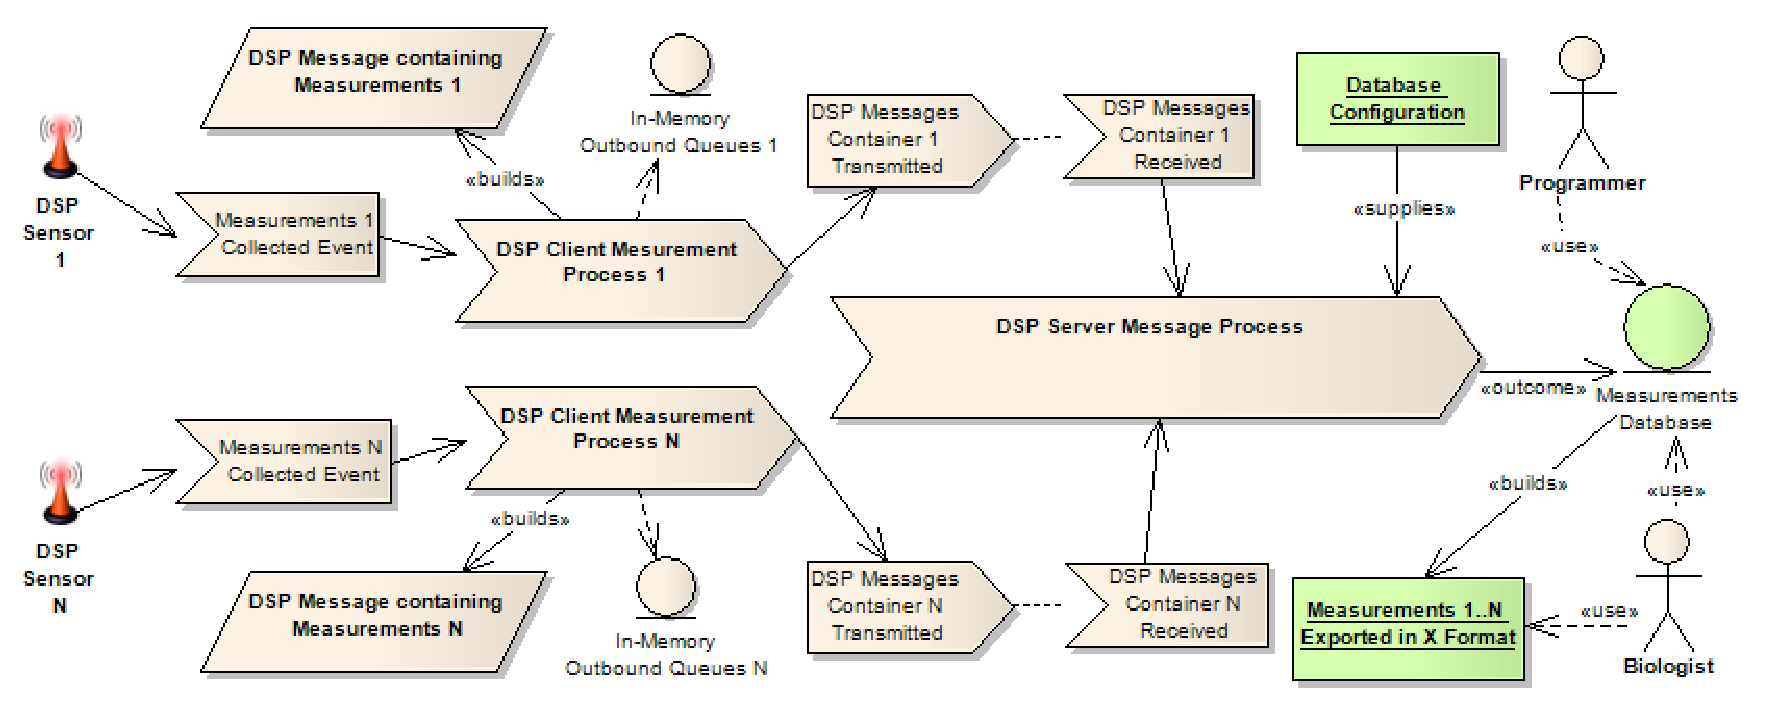
\includegraphics[scale=0.6]{../diagrams/DSP-DataPersistence-Business-Diagram}
  \caption{UML Business Process Model diagram - Adding Persistence for NetBEAMS}
  \label{fig:dsp-persistence-business-process}
\end{figure}

The goal of the new DSP Data Persistence component is to proxy the payload 
from the DSP Messages to the new suggested Measurements Database. Once the DSP
Server receives all the messages in a container, it processes the messages and
sends their payloads to the Measurements Database. This process requires a new
Database Configuration to be provided to the DSP Server host, as well as the
installation and setup of the new Measurements Database. In this way, different
users of the collected data, such as Programmers and Biologists, can access the
collected data directly from the Measurements Database and reuse them by
Exporting specific observation parameters to different formats of their
interest.

\section{Requirements Specification}

This section outlines the functionalities and constraints that the developed
solution must perform and follow, respectively, obtained by analyzing the main
data collection scenario described in the previous section and reviewing the
requirements defined by the RTC staff members.

\subsection{Functional Requirements}
\label{sec:use-cases}

The primary goal of the system is to allow users to have easy access to the 
collected data from \emph{NetBEAMS} using a schema-less database technology.
mongoDB provides access to the stored data without requiring the use of 
a Structured Query Language. Instead, that technology provides a programming
language abstraction that makes the access to the stored data easier 
\cite{sn-programming-language}. Using Agile User Stories to describe Use 
Cases Diagrams \cite{use-cases-user-stories}, Figure 
\ref{fig:DSP-Data-Persistence-UseCases-Diagram-Users} enumerates these
functionalities as customers conversations, starting with a fictitious
persona, the action it desires to perform and the outcome of the action, a
requirements gathering pattern defined in Scrum \cite{agile-scrum}:

\begin{figure}[!b]
  \centering
  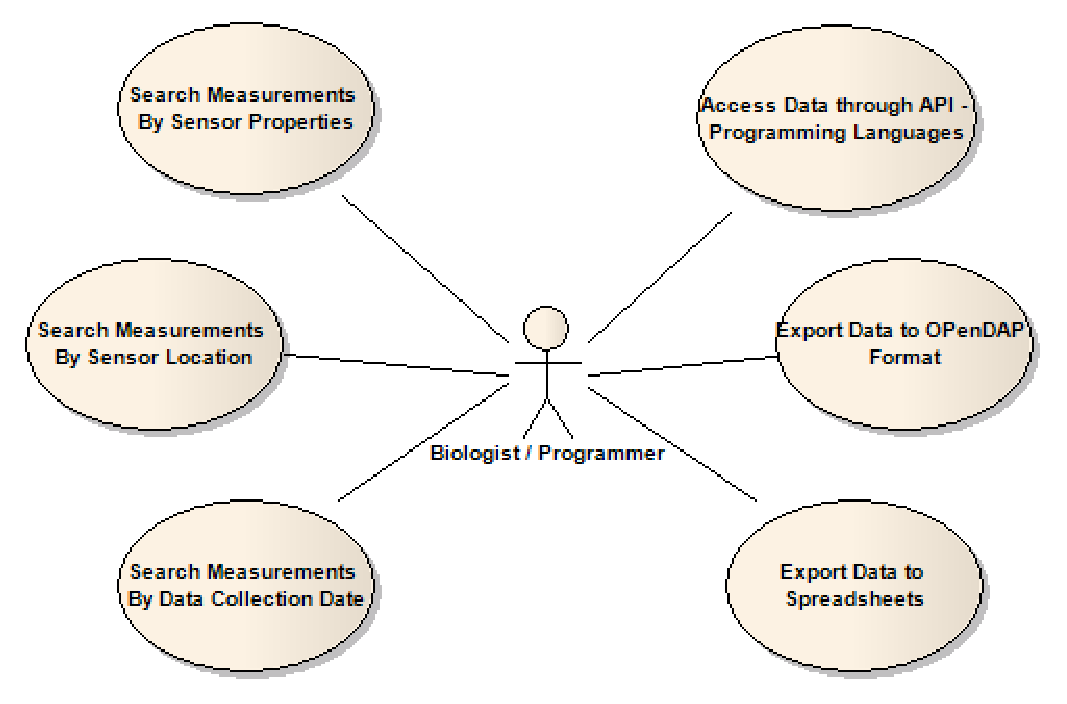
\includegraphics[scale=0.65]{../diagrams/DSP-Data-Persistence-UseCases-Diagram-Users}
  \caption{UML Use Case diagram for Persistence Functions}
  \label{fig:DSP-Data-Persistence-UseCases-Diagram-Users}
\end{figure}

\begin{itemize}
  \item \textbf{Search Measurements by Sensor Properties}: "As a marine
  biologist, I would like to search observations by filtering values of the 
  sensor device's properties such as temperature or salinity, so that I can 
  find specific associated values to the observation.";
  \item \textbf{Search Measurements by Sensor Location}: "As an oceanographer,
  I would like to search observations that took place at the geographic
  coordinates (x latitude, y longitude), so that I can assess the area around
  the given coordinates.";
  \item \textbf{Search Measurements by Data collection date}: "As a marine 
  biologist, I would like to search observations that took place last week, 
  so that I can assess past environmental conditions";
  \item \textbf{Annotate Existing Measurements}: "As a estuarine ecologist,
  I would like to annotate observations from the time the oil spill occurred
  in the San Francisco Bay, so that I can maintain historical evidence of 
  the impact of such event.";
  \item \textbf{Export Data to Spreadsheets}: "As a scientist from RTC, I 
  would like to analyze of the observed data from yesterday using a 
  spreadsheet, so that I can verify measurements using Microsoft Excel.";
  \item \textbf{Export Data to OPeNDAP format}: "As a biologist, I would 
  like to export the collected data produced during this month using the
  OPeNDAP data format, so that I can collaborate with other research groups
  that uses this data format.";
  \item \textbf{Access the data through API, Programming Languages}: "As a
  marine biologist who learned the Python scripting language, I would like to
  write a software that connects directly to the database, so that I can
  implement a customized analysis system for NetBEAMS.";
  \item \textbf{Remove Undesired Measurements}: "As an oceanographer, I
  would like to remove specific observations collected yesterday, 
  so that the research group does not use 'junk data'.".
\end{itemize}

As one can see, the basic users' functionalities are related to the access to
the collected data using different parameters related to the each observation's
properties or implied metadata such as time of collection or location. In order
to do so, the functions to be performed were developed following the
specifications of the Data Sensor Platform (DSP) architecture, as described in
\cite{netbeams-dsp-architecture}. In order to collect data sent to the NetBEAMS
server, the new DSP component must act as a Data Consumer. The functionalities
provided by this component can be seen in the UML Use Cases diagram \cite{uml}
in Figure \ref{fig:DSP-Data-Persistence-UseCases-Diagram-System}, and
summarized as follows:

\begin{figure}[!h]
  \centering
  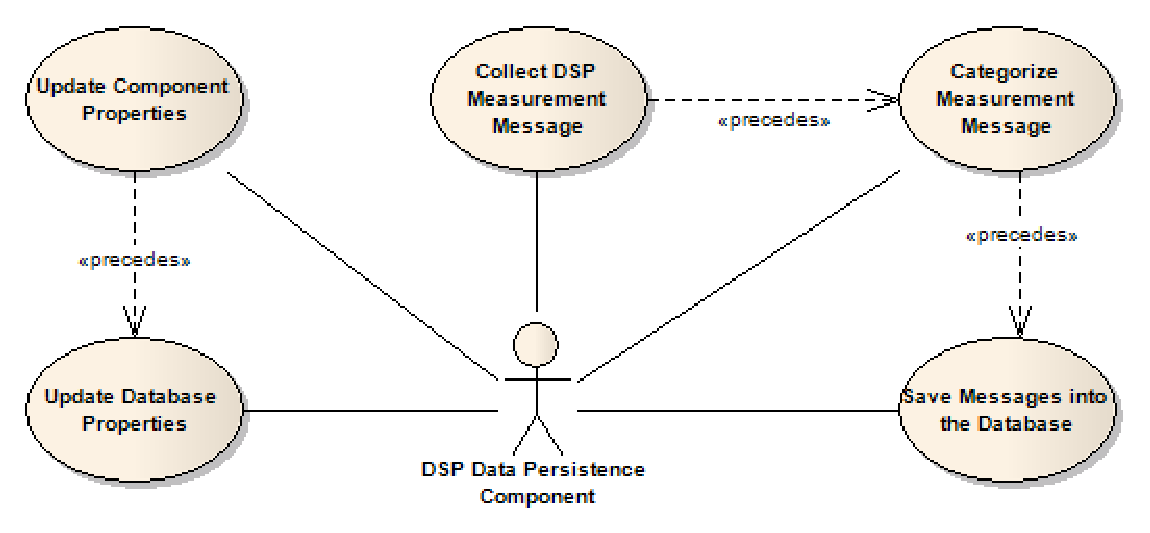
\includegraphics[scale=0.65]{../diagrams/DSP-Data-Persistence-UseCases-Diagram-System}
  \caption{UML Use Case diagram for the Persistence Component}
  \label{fig:DSP-Data-Persistence-UseCases-Diagram-System}
\end{figure}

\begin{itemize}
  \item \textbf{Update Component Properties}: the component must be
  configurable, with its own set of properties, such as the flush rate used 
  to send data to the database system;
  \item \textbf{Update Database Properties}: the component must be able to
  update the mongoDB database settings such as IP Address and  communication 
  port;
  \item \textbf{Collect DSP Measurement Message}: the component must be
  able to receive and temporarily retain the collected messages from
  different the sensors devices;
  \item \textbf{Categorize Measurement Message}: the component must be able
  to categorize the DSP Message, as it arrives, by its properties such as 
  transaction time, and originating DSP Message ID;
  \item \textbf{Save Messages into the Database}: the component must be able
  to send the payload of the DSP Messages to the database.
\end{itemize}

\subsection{Non-Functional Requirements}

Different constraints were required to execute the functional requirements
described in the previous section. Those constraints are listed as different
non-functional requirements as follows:

\begin{itemize}
  \item The solution must maintain the received DSP Measurement Messages
  in-memory for a specific period of time in order to decrease the write load
  on the database (flush rate);
  \item The persistence storage system must be able to cope with the Data
  Volume produced by SF-BEAMS on daily basis;
  \item The persistence storage system must be able to scale without minimal
  architectural and schema changes;
  \item The persistence storage system must be able to provide access to the
  persisted data using an programmatic abstraction interface, as the authors
  of \cite{sn-programming-language} proposed.
\end{itemize}

Driven by the requirements defined, the foundation of the integration between
the DSP Data Persistence component and the mongoDB database system is the
specification of the Keys that comprise a set of observations collected from
the sensor devices.

\section{Data Model Design}
\label{sec:dsp-persistence-data-model}

MongoDB is defined as a Document-Oriented Database system, which is based on 
the abstraction of the Key-Value-Pair data model, using a binary version of JSON
\cite{json} as its main data representation. MongoDB does not require the creation 
of a database schema, rather the definition of key descriptions that comprises
a document on the database organized into separate collections of relating
documents. In order to describe the keys of a document, the specifications
detail the use of Data Provenance as guidelines to the description of the
collected data. Therefore, the key-value pairs of any instance of the
collected data must include the following key properties:

\begin{itemize}
  \item \textbf{Location}: properties that describe the location of the data.
  For example, the host machine name, IP address, or the GPS coordinates
  \cite{gps} from the sensor device;
  \item \textbf{Identity}: what uniquely identifies the data among 
  others, produced by other sensor devices in the network such as the DSP
  Message ID using UUID\footnote{Universally Unique Identifier};
  \item \textbf{Time-Dimensions}: when the data was recorded 
  \cite{db-provenance} and when the transaction occurred \cite{sn-time-series}.
\end{itemize}

After analyzing the DSP Platform and the structure of the DSP Messages in
\cite{netbeams-dsp-architecture}, the values of the collected data must be
categorized into two different sets of data: the ``Key Segment'' and the
``Value Segment''. The key segment provides the necessary metadata 
used to describe the collected data. An instance of the design of the 
keys is shown in Listing \ref{file:mongodb-ysi-data-format}:

\begin{itemize}
  \item \textbf{message\underline{ }id}: Defines the DSP Message ID that
  carried the observation from the sensor device to the DSP Server. This ID
  can be used during network and database inspections in order to track messages
  for the DSP Platform;
  \item \textbf{sensor}: Defines the properties of the sensor device;
    \begin{itemize}[label=\textbullet]
        \item \textbf{ip\underline{ }address} Defines the IP Address of the 
        sensor device that produced the data;
        \item \textbf{location}: Defines the geographical coordinates of the
        sensor device, using the Decimals Degree format \cite{decimal-degrees};
            \begin{itemize}[label=\textbullet]
                \item \textbf{latitude} the GPS latitude coordinate of the
                position of the sensor device;
                \item \textbf{longitude}: the GPS longitude coordinate of the
                position of the sensor device.
            \end{itemize}
    \end{itemize}
  \item \textbf{time}: Defines different time dimensions according to Data 
   Provenance;
    \begin{itemize}[label=\textbullet]
      \item \textbf{valid}: it is extracted from the container's date and time
      of creation, which was collected during the sensor device's reading;
      \item \textbf{transaction}: it is extracted from the DSP message
         container's creation time and it is used to identify when the
         transaction, which transferred the message from the DSP Gateway Client
         to the DSP Server, occurred;
    \end{itemize} 
\end{itemize}

An associated ``Value Segment'' for the aforementioned ``Key Segment'' carries
the observations of a given sensor device. The key \textbf{observation} stores
the values of the collected data. For instance, the observation key of
for the YSI device \cite{YSI-Sonde} may contains all the subsets of 
the properties defined for the device, such as battery, temperature and
salinity, among others. An example of such use of the segments is shown in
Listing \ref{file:mongodb-ysi-data-format}.

Based on this foundation, the design of the DSP Data Persistence component
evolved from a top-down approach.

\section{High-Level System Architecture}

Considering the business analysis described in Section
\ref{sec:business-process-analysis}, the addition of a data persistence layer
to the DSP Platform can be achieved by adding a Data Consumer (DC) as 
described by \cite{netbeams-dsp-architecture}. Based on the 
Requirements specification, this component must be responsible for the 
extraction process that takes the payload of the body of a filtered DSP
Measurement Message and converts it to the key-value data model defined
in the previous section. This process guarantees that the collected data is
inserted to a running mongoDB database system and gives covers the use cases
defined. Figure \ref{fig:NetBEAMS-Persistence-Server-Node-Components}
provides an architectural overview of the DSP Server node with the
loosely-coupled components, highlighting the inclusion of a new DSP Component
called ``DSP Data Persistence''.

\begin{figure}[!h]
  \centering
  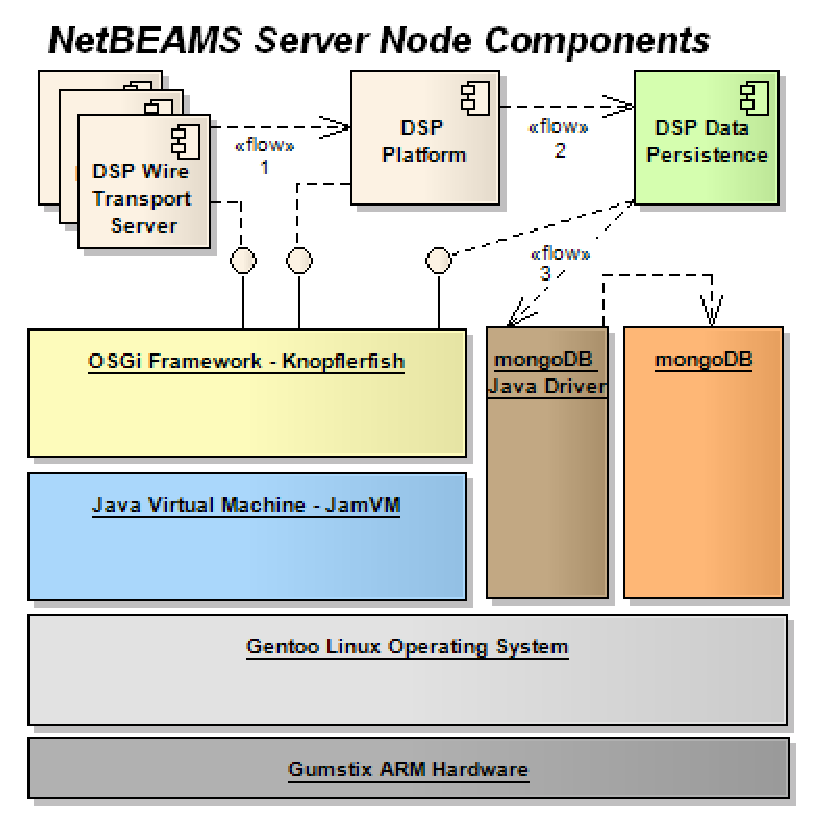
\includegraphics[scale=0.65]{../diagrams/NetBEAMS-Persistence-Server-Node-Components}
  \caption{UML Components diagram of the DSP Data Collector}
  \label{fig:NetBEAMS-Persistence-Server-Node-Components}
\end{figure}

As it is depicted the diagram 
\ref{fig:NetBEAMS-Persistence-Server-Node-Components}, the DSP Data
Persistence can be added into the existing architecture as an 
independent plug-and-play component. The database system and the necessary
drivers are also added without any changes to the existing DSP 
infrastructure. First, the DSP Messages are delivered to the DSP server 
through the DSP Wire Transport Server, as shown by flow 1. Next, the DSP 
Platform is responsible to forward a copy of the Measurement messages 
directly to the DSP Data Persistence as shown by flow 2. Then, the sole 
responsibility of the DSP Data Persistence is to transfer the received 
measurement messages to the database system by using the connection 
drivers, as shown by flow 3.

Any DSP Component is essentially an OSGi Bundle \cite{osgi-intro}, a unit of
deployment in a Java JAR format \cite{java-tutorial} containing the Java
classes and a descriptor manifest artifact that identifies the major components
of the package, which services the component requires to use and which ones it
will optionally publish during its activation and lifecycle. Details about the
deployment of the DSP Data Persistence component, as well as about the OSGi
environment used, are given in the Appendix section
\ref{sec:dsp-component-osgi-deployment}.

The following sections focus on the DSP Data Persistence component 
design in the context of an OSGi bundle \cite{osgi}.

\section{DSP Data Persistence: OSGi-DSP Bundle Design}

The proposed Data Persistence component must follow the DSP Component
requirements, which specifies the design-pattern of Data Producer and Consumer
mentioned earlier in this chapter. As seen in the UML Package  Dependency
Diagram in Figure \ref{fig:DSP-Data-Persistence-Packages-Dependency}, a new
DSP Component has dependency on three different packages: the OSGi Framework
and the DSP Platform responsible to integrate a new component into the
micro-kernel, and the mongoDB Java driver API that connects to the mongoDB
server.

\begin{figure}[!h]
  \centering
  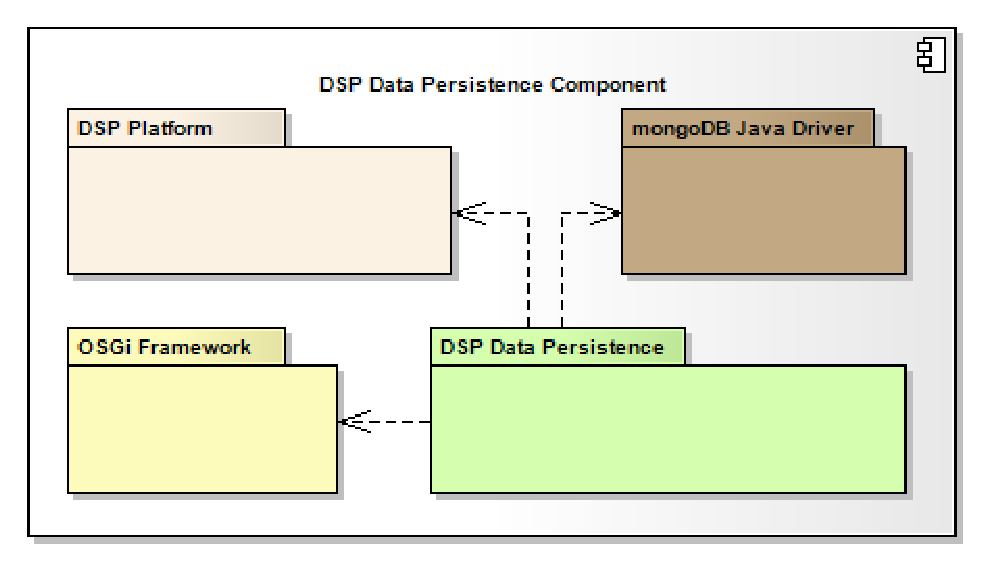
\includegraphics[scale=0.65]{../diagrams/DSP-Data-Persistence-Packages-Dependency}
  \caption{UML Components diagram of the DSP Data Collector}
  \label{fig:DSP-Data-Persistence-Packages-Dependency}
\end{figure}

In order to use a DSP Component, one must first activate it into the OSGi
Framework the DSP Platform runs on. Both the activation and the design of how
the new component acts as a Data Consumer is explained in the following
sections.

\subsection{DSP Data Persistence Activation and Message Delivery}

The DSP Data Persistence component starts with an OSGi Activator class, and 
the implementation of the DSP Component, responsible for providing services 
to the platform \cite{netbeams-dsp-architecture}. Based on these 
specifications, the following set of classes, shown in Figure 
\ref{fig:DSP-DataPersistence-Activator-Class-Diagram}, depicts the implemented
classes for the new DSP Data Persistence component.

\begin{figure}[!h]
  \centering
  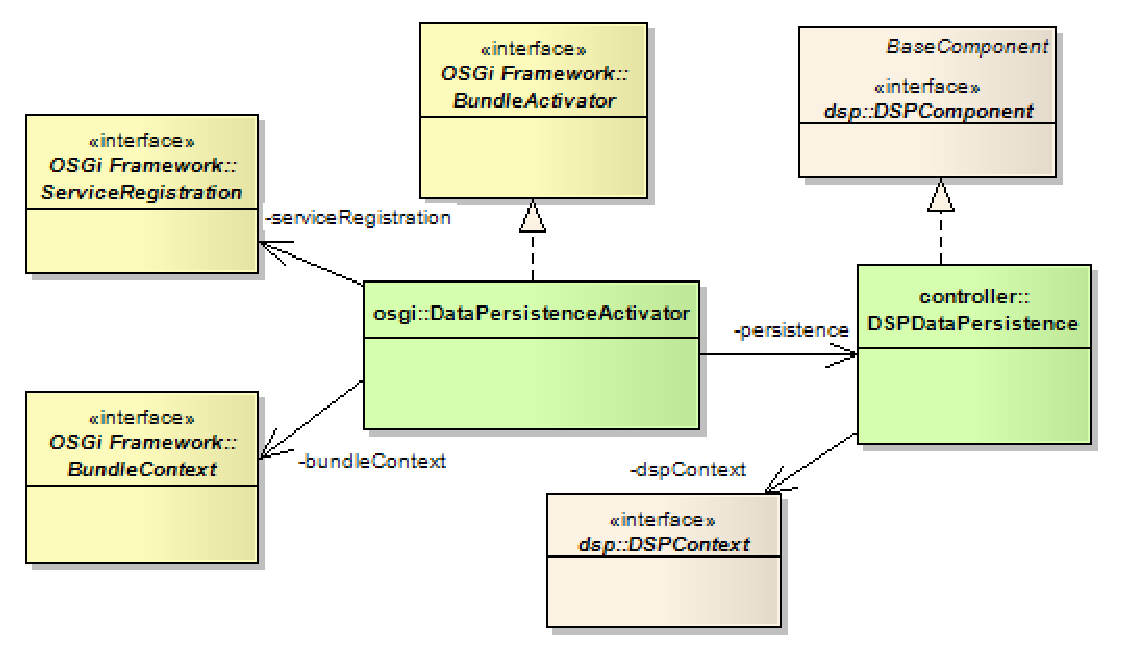
\includegraphics[scale=0.65]{../diagrams/DSP-DataPersistence-Activator-Class-Diagram}
  \caption{UML Class diagram for the DSP Data Persistence Activator and Component}
  \label{fig:DSP-DataPersistence-Activator-Class-Diagram}
\end{figure}

The class DSPDataPersistenceActivator is the main class responsible for the
activation of the class DSPDataPersistence, as it extends from the OSGi
class BundleActivator. The BundleActivator maintains references to the classes
BundleContext and ServiceReference, both from the OSGi Framework, in order to
maintain the component managed by the OSGi Framework and register the class
DSPDataPersistece as a service to the OSGi environment. Therefore, the class
DSPDataPersistenceActivator is the main communication interface between the 
DSP Platform and the OSGi Framework, are responsible for the orchestration of
the application lifecycle.

The class DSPDataPersistence implements the interface DSPComponent, responsible
to provide the contract between the component and the DSP platform. As a
consequence, this class inherits all the behavior described in
\cite{netbeams-dsp-architecture} necessary to be executed in the DSP Platform
in a given context (through the instance of class DSPContext). The different
roles played by the class DSPDataPersistence are defined as follows:

\begin{itemize}
  \item \textbf{Data Consumer}: receives any measurement message from remote
  sensors;
  \item \textbf{Data Producer}: transforms any received measurement message
  into the format defined in Section \ref{sec:dsp-persistence-data-model}, in
  order to be sent to the database.
\end{itemize}

The class DSPDataPersistenceActivator is responsible for starting and stopping,
the services provided by the DSPDataPersistence component, as this behavior is
inherited from the OSGi class BundleActivator from OSGi Framework. Following
the specification of the DSP Architecture \cite{netbeams-dsp-architecture},
Figure
\ref{fig:From-OSGi-Framework-to-DSP-Data-PersistenceActivator-Sequence-Diagram} 
shows a UML Sequence Diagram that depicts the steps of the activation of the
DSP component, and summarized as follows:

\begin{figure}[!h]
  \centering
  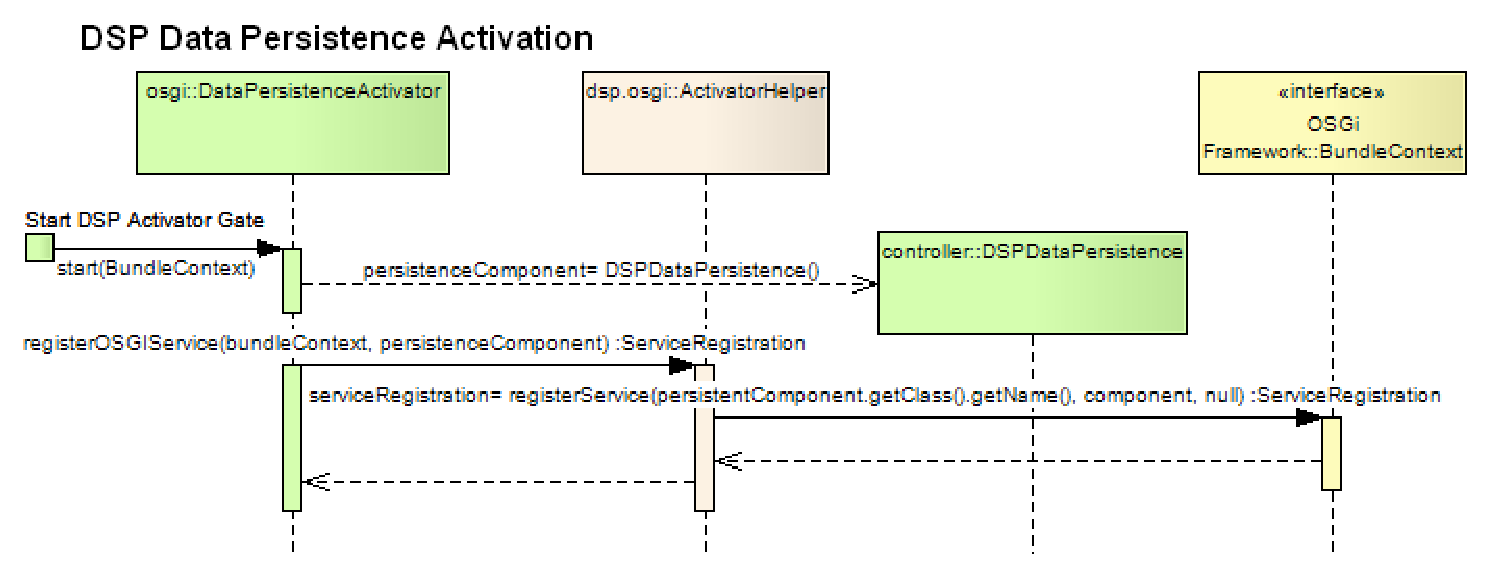
\includegraphics[scale=0.65]{../diagrams/From-OSGi-Framework-to-DSP-Data-PersistenceActivator-Sequence-Diagram}
  \caption{UML Sequence diagram describing the DSP Data Persistence bundle activation}
  \label{fig:From-OSGi-Framework-to-DSP-Data-PersistenceActivator-Sequence-Diagram}
\end{figure}

\begin{enumerate}
  \item During its activation, the DSP Platform will get the name of the
  DSP Data Persistence component from the configuration artifact config.xml as
  seen in Listing \ref{file:dsp-config.xml};
  \item After being selected based on the configuration priority, the 
  DSPBundle artifact is identified and installed by creating an instance of the
  class DSPDataPersistenceActivator, making a call to the method start();
  \item During the activation, an instance of the class DSPDataPersistence
  is created and registered as an OSGi Service;
  \item Upon registering the DSP Data Persistence component, the DSP Platform
  listens for the event serviceUpdate() and triggers the last operations to
  bootstrap the DSP Component:
   \begin{enumerate}
      \item Initialize the component by calling the method initComponent();
      \item Start the component by calling the method startComponent();
      \item Bootstrap messages by calling the method delivery(). This is where
      both the DSP Measurements Messages and Update Messages are delivered by
      the DSP Broker. This concept is based on the listener of Observer
      Design-Pattern \cite{gof}.
   \end{enumerate}
\end{enumerate}

Any configuration parameter required by a DSP Component is sent during its
bootstrap process through the use of an optional DSP Update Message, as shown
in Listing \ref{file:dsp-data-persistence-bootstrap.xml}. The initialization of
the DSP Component Activator and the DSP Component registration are also shown
in Figure \ref{fig:From-OSGi-Framework-to-DSP-Data-PersistenceActivator-Sequence-Diagram}.

As soon as the process "Start DSP Activator Gate" is executed, an instance of
the class DSPDataPersistence component is created to be registered into the
OSGi Framework using the DSP Platform's helper class ActivationHelper. It is
responsible to proxy the method call to the class BundleContext, which makes
the actual registration of the DSPDataPersistence component as an OSGi
Service. At this point, the DSPDataPersistence is installed and on the state
"Active", as defined by the OSGi Framework (Refer to
\cite{netbeams-dsp-architecture} for details).

Once the DSP Data Persistence component is concurrently running with other
components from both the DSP Platform and the OSGi Framework, it is able to
receive DSP Messages. The following section will explain how to bootstrap the
DSP Data Component in order to receive Measurement Messages.

\subsection{Delivering Bootstrap and Measurement Messages}

Although the DSP Data Persistence component has been instantiated as of Figure
\ref{fig:From-OSGi-Framework-to-DSP-Data-PersistenceActivator-Sequence-Diagram}, 
the process of delivering messages to the DSP Data Persistence component has yet
to be completed. As defined by the requirements, the DSP Component must execute its
function concurrently, using the configuration parameters during its
bootstrap process. The DSP Platform delivers any bootstrap message defined in
the DSP Platform runtime environment, as explained in the Appendix section
\ref{sec:dsp-persistence-boostrap}. However, to deliver DSP Measurement
Messages, a new filter must be provided. As explained in
\cite{netbeams-dsp-architecture}, the DSP Broker uses the DSP Matcher's rules
to select to Data Consumers configured in a given DSP. For this reason, a rule
that filters any remote measurement message received by running DSP Server is
used, as shown in Listing \ref{file:dsp-matcher-config.xml}. The rule defined
in line 63 express that all messages created by any producer on any DSP Host,
either client or sever, has as delivery target the DSP Data Persistence
component. In this way, when DSP Measurement Messages are delivered, the DSP
Broker delivers the DSP Message to the DSP Data Persistence Component.

The UML Class Diagram for the participating classes of the DSP Data
Persistence component is shown in Figure
\ref{fig:DSP-DataPersistence-Flusher-Classes}. The class DSPDataFlusher is
responsible for running as a worker thread, whose function is to verify if
there are messages to be flushed to the Database by contacting the Singleton
class \cite{gof} TransientPersistenceLayer, responsible to keep track of the
DSP Messages received when the DSP Broker delivered them to the DSP Data
Persistence component.

\begin{figure}[!h]
  \centering
  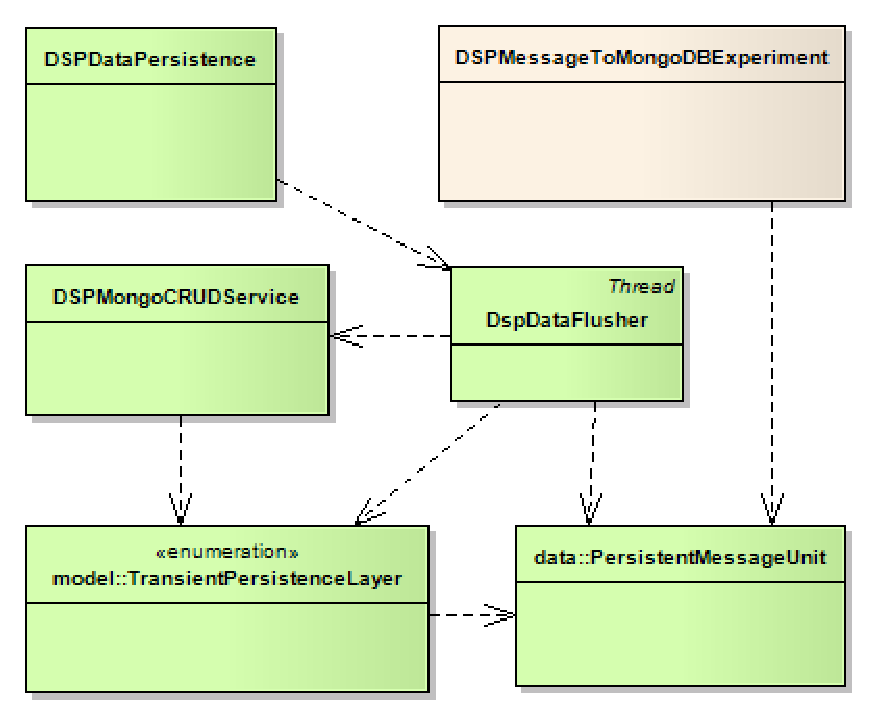
\includegraphics[scale=0.65]{../diagrams/DSP-DataPersistence-Flusher-Classes}
  \caption{UML Class diagram with DSP Data Persistence and Participating classes}
  \label{fig:DSP-DataPersistence-Flusher-Classes}
\end{figure}

Upon receiving a new DSP measurement message, the DSP Data Persistence
component keeps any received message in a temporary local cache, as described 
by the non-functional requirements. In this way, the DSP Data Persistence 
component maintains a dependency on the Singleton class TransientPersistenceLayer, 
responsible for encapsulating the DSP Message into an instance of the class 
PersistentMessageUnit, to be stored in the defined local cache.

According to the DSP Broker model described in \cite{netbeams-dsp-architecture}, 
the DSP Matcher needs to be updated with the addition of a matching rule that
filters a copy of any Measurement Message to the DSP Data Persistence component. 
As it is shown in Figure
\ref{fig:From-DSP-Broker-To-DSPDataPersistence-General-Sequence}, the worker
Thread DSP Data Flusher is the link between the Transient and Persistent
layers, as it depends on the references from the classes
TransientPersistenceLayer and the DSPMongoCRUDService.The class
DSPMongoCRUDService is responsible for extracting the collected data from the
body of the DSP Message and creating the keys designed to be persisted
in the mongoDB Database.

The DSP Broker retrieves the list of matching rules by contacting the Matcher.
As the DSP Platform has already loaded all the Matching rules, a copy of an
analyzed DSP Message is delivered to the DSP Data Persistence component specified
by a matcher rule. However, the UML Sequence Diagram depicted in Figure 
\ref{fig:From-DSP-Broker-To-DSPDataPersistence-General-Sequence} shows two 
different moments of message delivery:

\begin{figure}[!h]
  \centering
  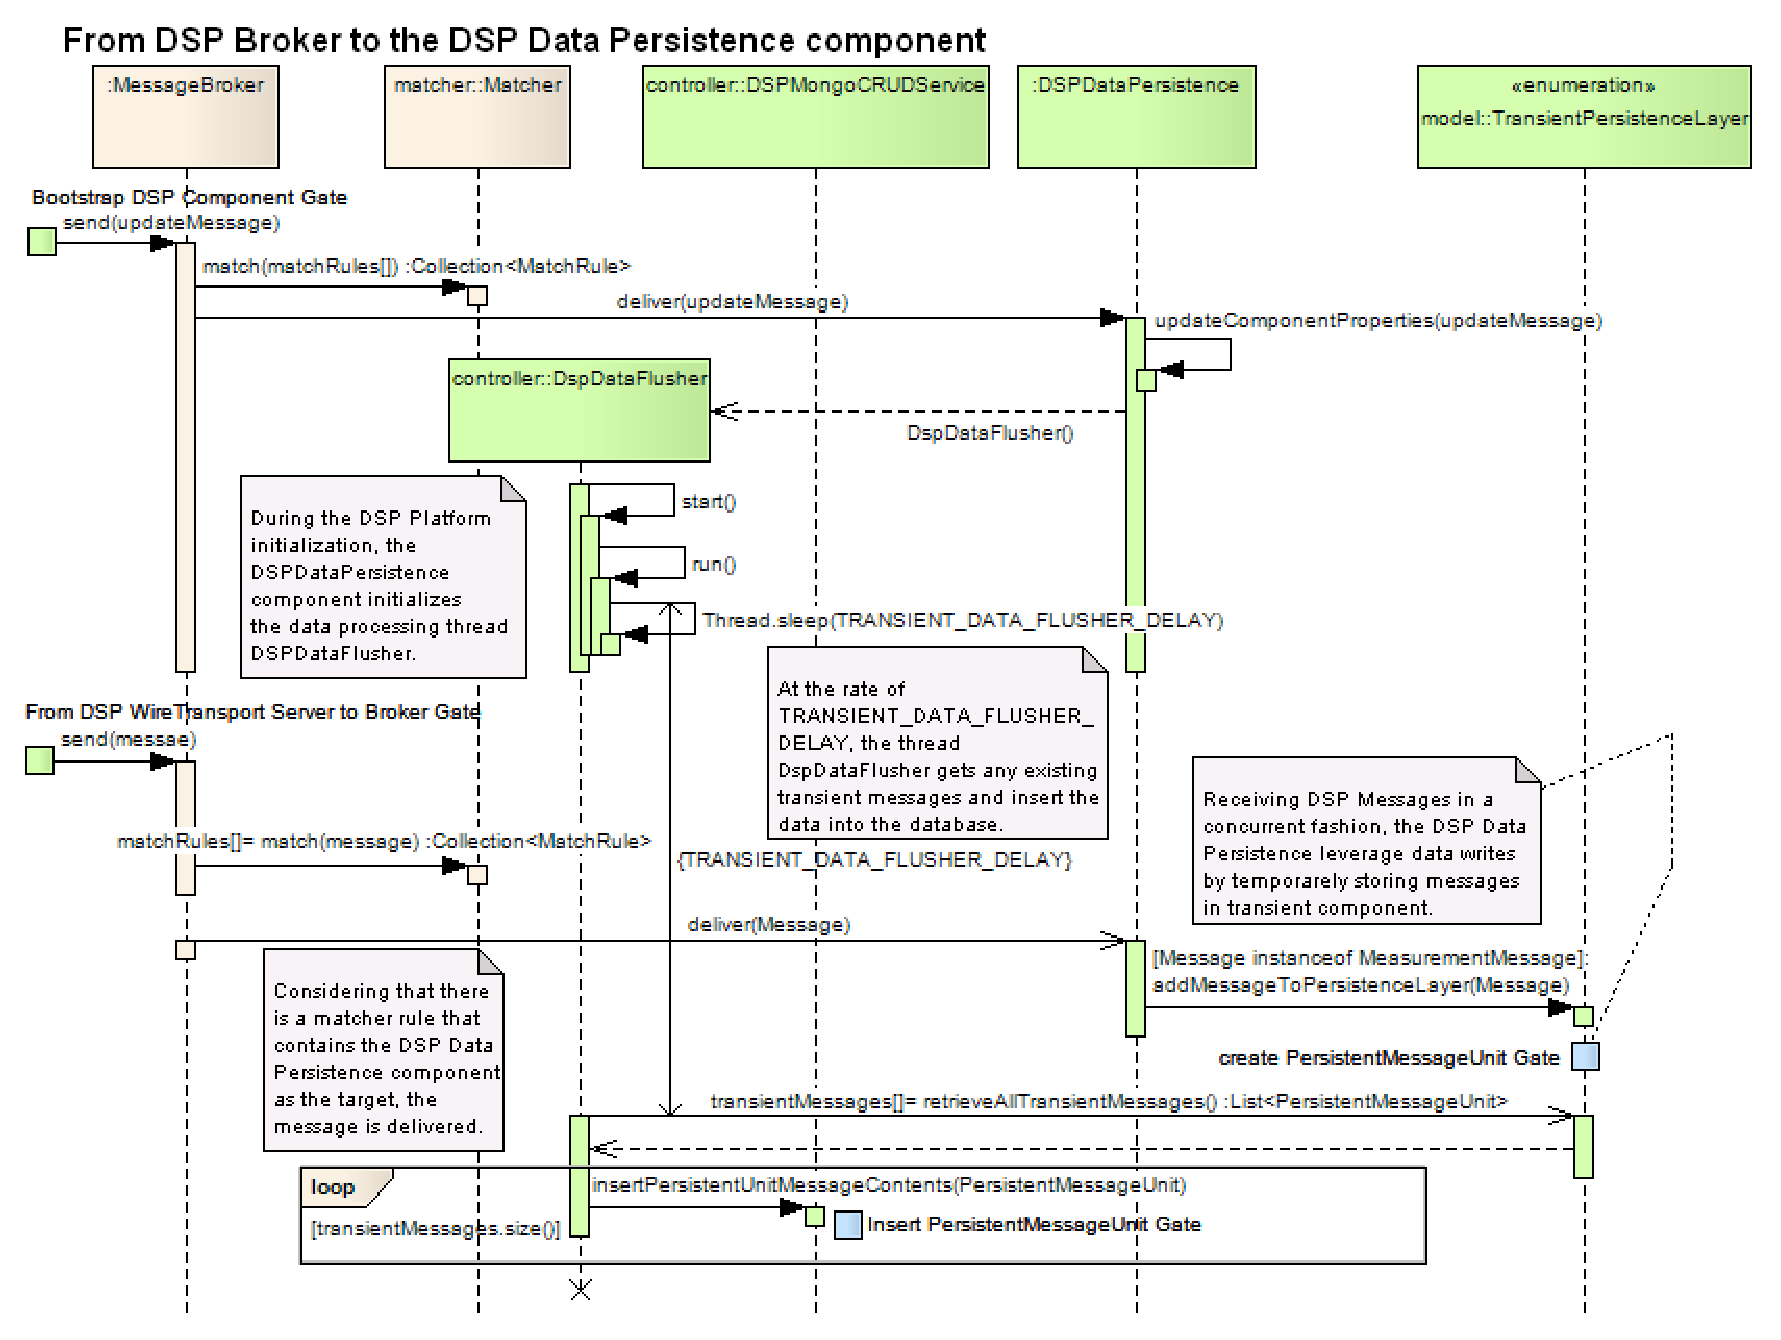
\includegraphics[scale=0.6]{../diagrams/From-DSP-Broker-To-DSPDataPersistence-General-Sequence} 
  \caption{UML Sequence Diagram - Flow 1: From the DSP Broker to the Data Persistence Component}
  \label{fig:From-DSP-Broker-To-DSPDataPersistence-General-Sequence}
\end{figure}

\begin{itemize}
  \item A bootstrap DSP Update Message is delivered to the DSP Data Persistence
  component when the DSP Platform is initializing the component. For example, the
  class DSPDataPersistence can initialize the class DspDataFlusher to
  flush temporary messages into the database at the rate of
  TRANSIENT\underline{ }DATA\underline{ }FLUSHER\underline{ }DELAY, defined in 
  seconds. 
  Listing \ref{file:dsp-data-persistence-bootstrap.xml} shows an
  implementation of a bootstrap message for the DSP Data Persistence;
  \item Any DSP Measure Message can be persisted by the DSP Data Persistence
  component. The component will add the message to a temporary memory location
  to decrease I/O on the database, when the DSP Broker delivers a DSP
  MeasureMessage to this component, as depicted by the gate "create
  PersistentMessageUnit Gate". This last gate describes the simple procedure
  to add the message into the transient persistent layer. Listing
  \ref{stream:dsp-message-serialized-ysi}.
\end{itemize}

The class PersistenceMessageUnit is the major transient persistence unit that
carries references regarding the originating DSP Message that was collected by
the DSP Data Persistence component. It is composed by an instance of the class 
SensorLocation and contains a reference to the PersistentMessageState
enumeration. The former identifies which sensor produced the collected data
from the DSP Message by the IP address, while the latter identifies whether
the PersistenceMessageUnit has been saved into the Database or not as depicted
by the UML State Diagram in Figure \ref{fig:PersistentMessageState-Diagram}. 
The class SensorLocation was developed as a to facilitate the identification of
sensor devices that are not capable of sampling their geographical location by
giving their references during the bootstrap process.

\begin{figure}[!h]
  \centering
  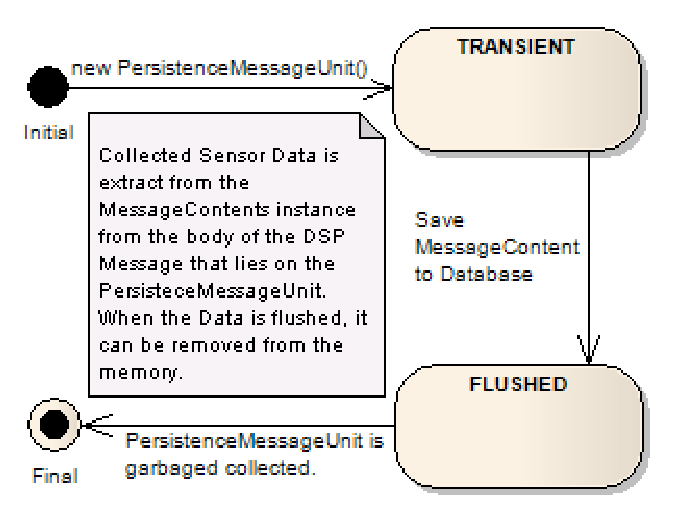
\includegraphics[scale=0.65]{../diagrams/PersistentMessageState-Diagram}
  \caption{UML State Diagram for the instance of the class
  PersistentMessageState}
  \label{fig:PersistentMessageState-Diagram}
\end{figure}

When a DSP Message is delivered to the DSP Data Persistence component, the
message is directly transferred to the Singleton class
TransientPersistenceLayer, as described before. As described in the UML
Sequence Diagram in Figure
\ref{fig:From-Create-PersistentMessageUnit-to-TransientPersistence-Layer-Sequence},
the first point of execution is the ``create PersistentMessageUnit Gate'',
where an instance of the SensorLocation is acquired for any DSP Message
received, in order to be added into the local cache. Before that occurs, the
PersistentMessageUnit is placed in the state ``TRANSIENT''.

\begin{figure}[!b]
  \centering
  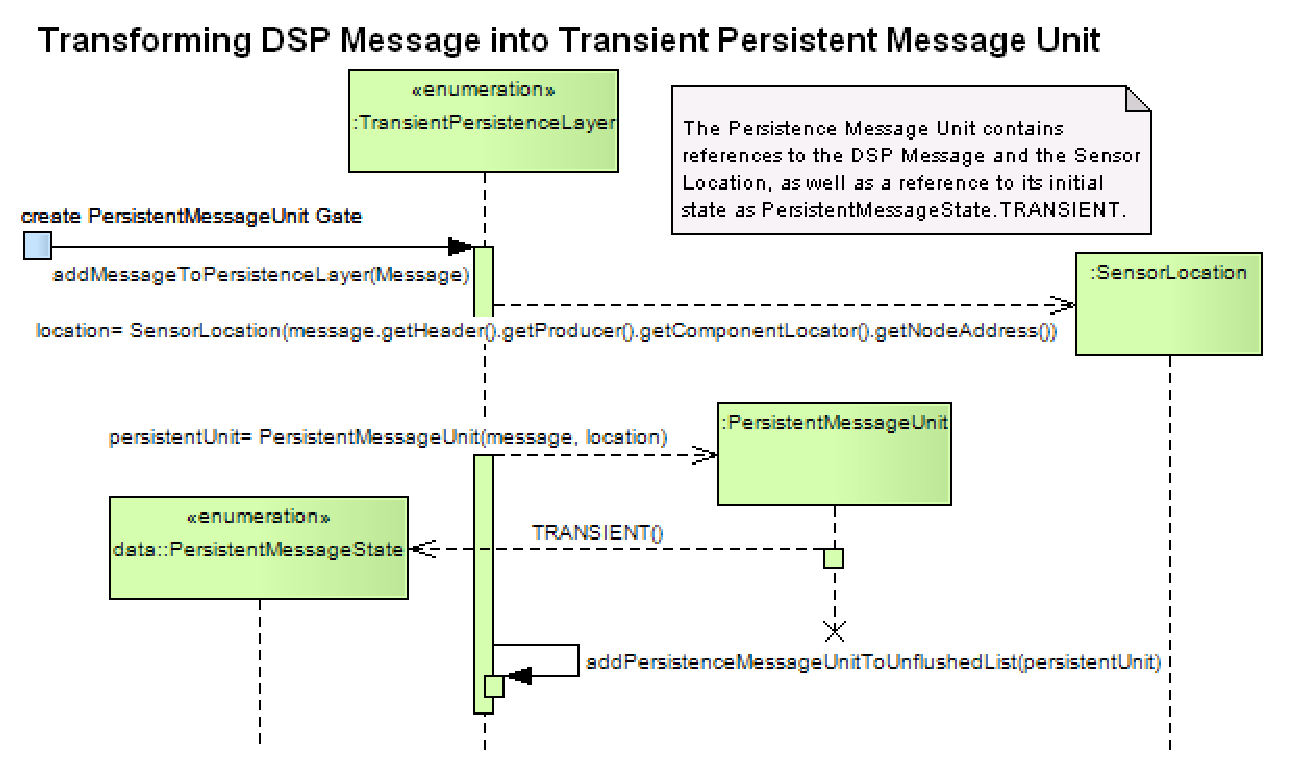
\includegraphics[scale=0.65]{../diagrams/From-Create-PersistentMessageUnit-to-TransientPersistence-Layer-Sequence}
  \caption{UML Sequence diagram - Adding a DSP Message into the Transient Persistence layer}
  \label{fig:From-Create-PersistentMessageUnit-to-TransientPersistence-Layer-Sequence}
\end{figure}

At this point, the DSP Data Persistence component maintains a set of DSP
Messages in a local cache during the specific ``flush rate'' specified during
the bootstrap message. When the class DSPDataFlusher finds any number of
instances of PersistentMessageUnit in cache, it starts the process of flushing
them into the mongoDB database, described in the following section.

\subsection{Flushing data into the Database}

The class DSPDataFlusher is a thread designed to be in two different states, as
depicted in Figure \ref{fig:DSP-DataPersistence-Flusher-State-Diagram}:

\begin{figure}[!h]
  \centering
  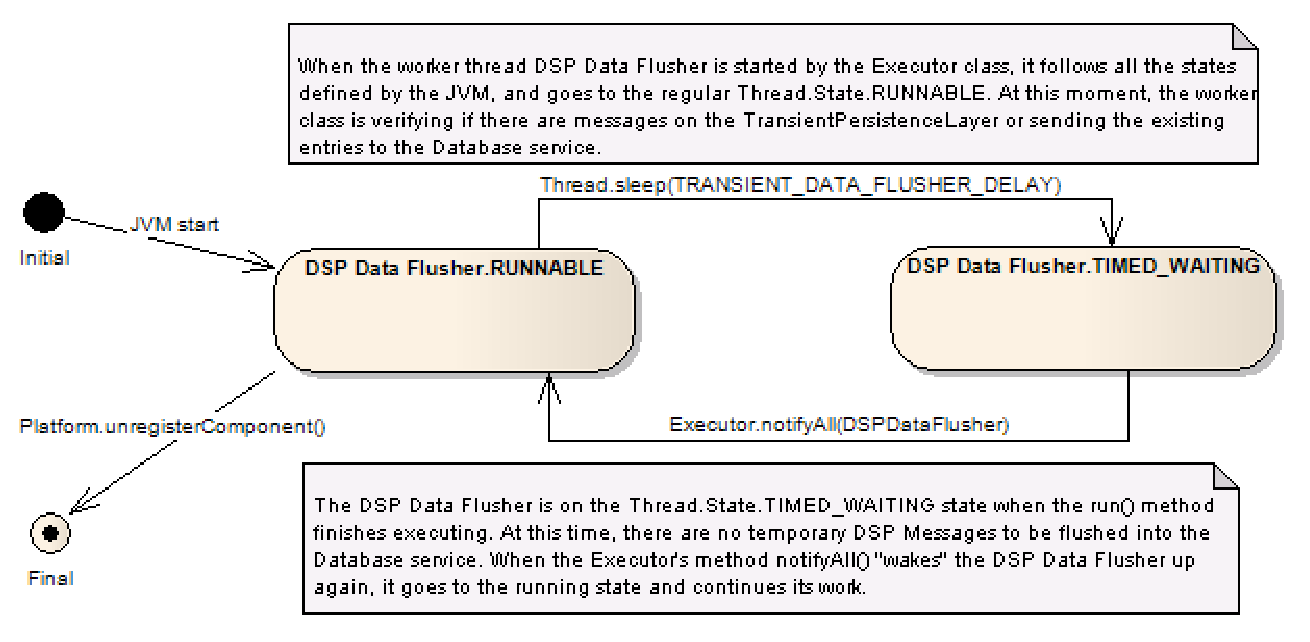
\includegraphics[scale=0.65]{../diagrams/DSP-DataPersistence-Flusher-State-Diagram}
  \caption{UML State diagram for the DSP Data Flusher Worker Thread}
  \label{fig:DSP-DataPersistence-Flusher-State-Diagram}
\end{figure}

\begin{itemize}
  \item \textbf{TIMED\underline{ }WAITING}: the initial state of a Java thread
  after its initialization, waiting to be on the ``runnable'' state. This
  period of time is defined by the ``flush rate''  specified in the bootstrap
  message of the DSP Data Persistence component;
  \item \textbf{RUNNABLE}: the class DSPDataFlusher contacts the class
  TransientPersistenceLayer, in order to verify if there are any instance of
  the class PersistentMessageUnit waiting to be transmitted from the temporary
  cache to the Database service. If the cache is not empty, the DSPDataFlusher 
  acquires the lock over the TransientPersistenceLayer and retrieves the
  existing set of PersistentMessageUnit to be sent to mongoDB. Then, it sends
  all of the PersistentMessageUnit classes to the Singleton Service class 
  DSPMongoCRUDService, which is responsible to extract the collected data from
  the DSP Message's Body and convert it to the Key-Value model specified in
  Section \ref{sec:dsp-persistence-data-model}.
\end{itemize}

The main participating classes from the DSPMongoCRUDService are shown in the
UML Class Diagram \ref{fig:DSP-Data-Persistence-Mongo-Classes}. It keeps references
to all types of sensor devices such as the SondeDataContainer and the
MouseActionsContainer. Furthermore, it is responsible to implement the CRUD
methods to modify the mongoDB database state. The class Mongo is used to acquire
an instance of the connection with mongoDB server and provide Factory Methods 
\cite{gof} to create instances of the classes DB, DBCollection and
BasicDBObject. The class DB is used as a reference to a database namespace, 
such as ``netbeams'', the one suggested and implemented by this work. Similarly,
class DBCollection offers an API to manipulate similar documents via the
abstraction of a collection of items. Finally, the class BasicDBObject is used
to represent the keys and values to be persisted in the database.

\begin{figure}[!h]
  \centering
  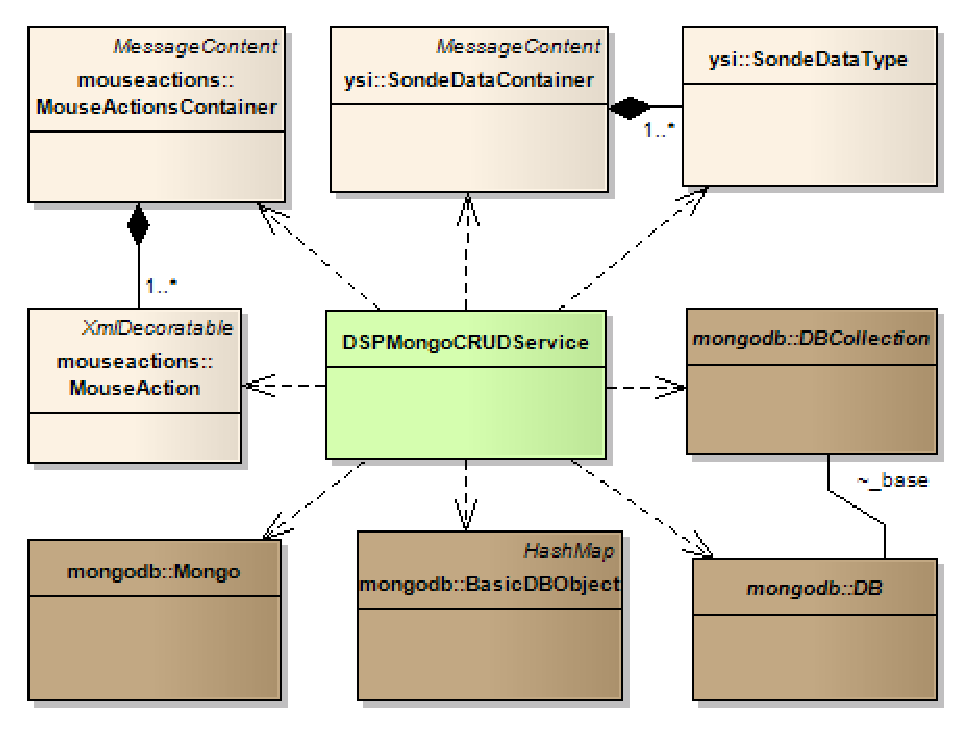
\includegraphics[scale=0.65]{../diagrams/DSP-Data-Persistence-Mongo-Classes}
  \caption{UML Class diagram with Persistence Service for MongoDB}
  \label{fig:DSP-Data-Persistence-Mongo-Classes}
\end{figure}

The last method call of the UML Sequence Diagram, depicted in Figure
\ref{fig:From-DSP-Broker-To-DSPDataPersistence-General-Sequence}, shows the
method call to the DSPMongoCRUDService method call to persist each of the
PersistentMessageUnit (see execution point ``addPersistentMessageUnit Gate'').
In short, the class DspDataFlusher continuously wakes up at the rate of
``TRANSIENT\underline{ }DATA\underline{ }FLUSHER\underline{ }DELAY''. Its
purpose is as simple as to iterate over the list of PersitenceMessageUnit on
the state of TRANSIENT, and send each of them to be saved on the persistence
storage. 

Finally, this sequence of events is continued by "inserting''
``PersistenceMessageUnit Gate", which triggers the persistence service from the
chosen database system as shown in Figure
\ref{fig:From-Insert-PersistentMessageUnit-to-mongoDB}.

\begin{figure}[!h]
  \centering
  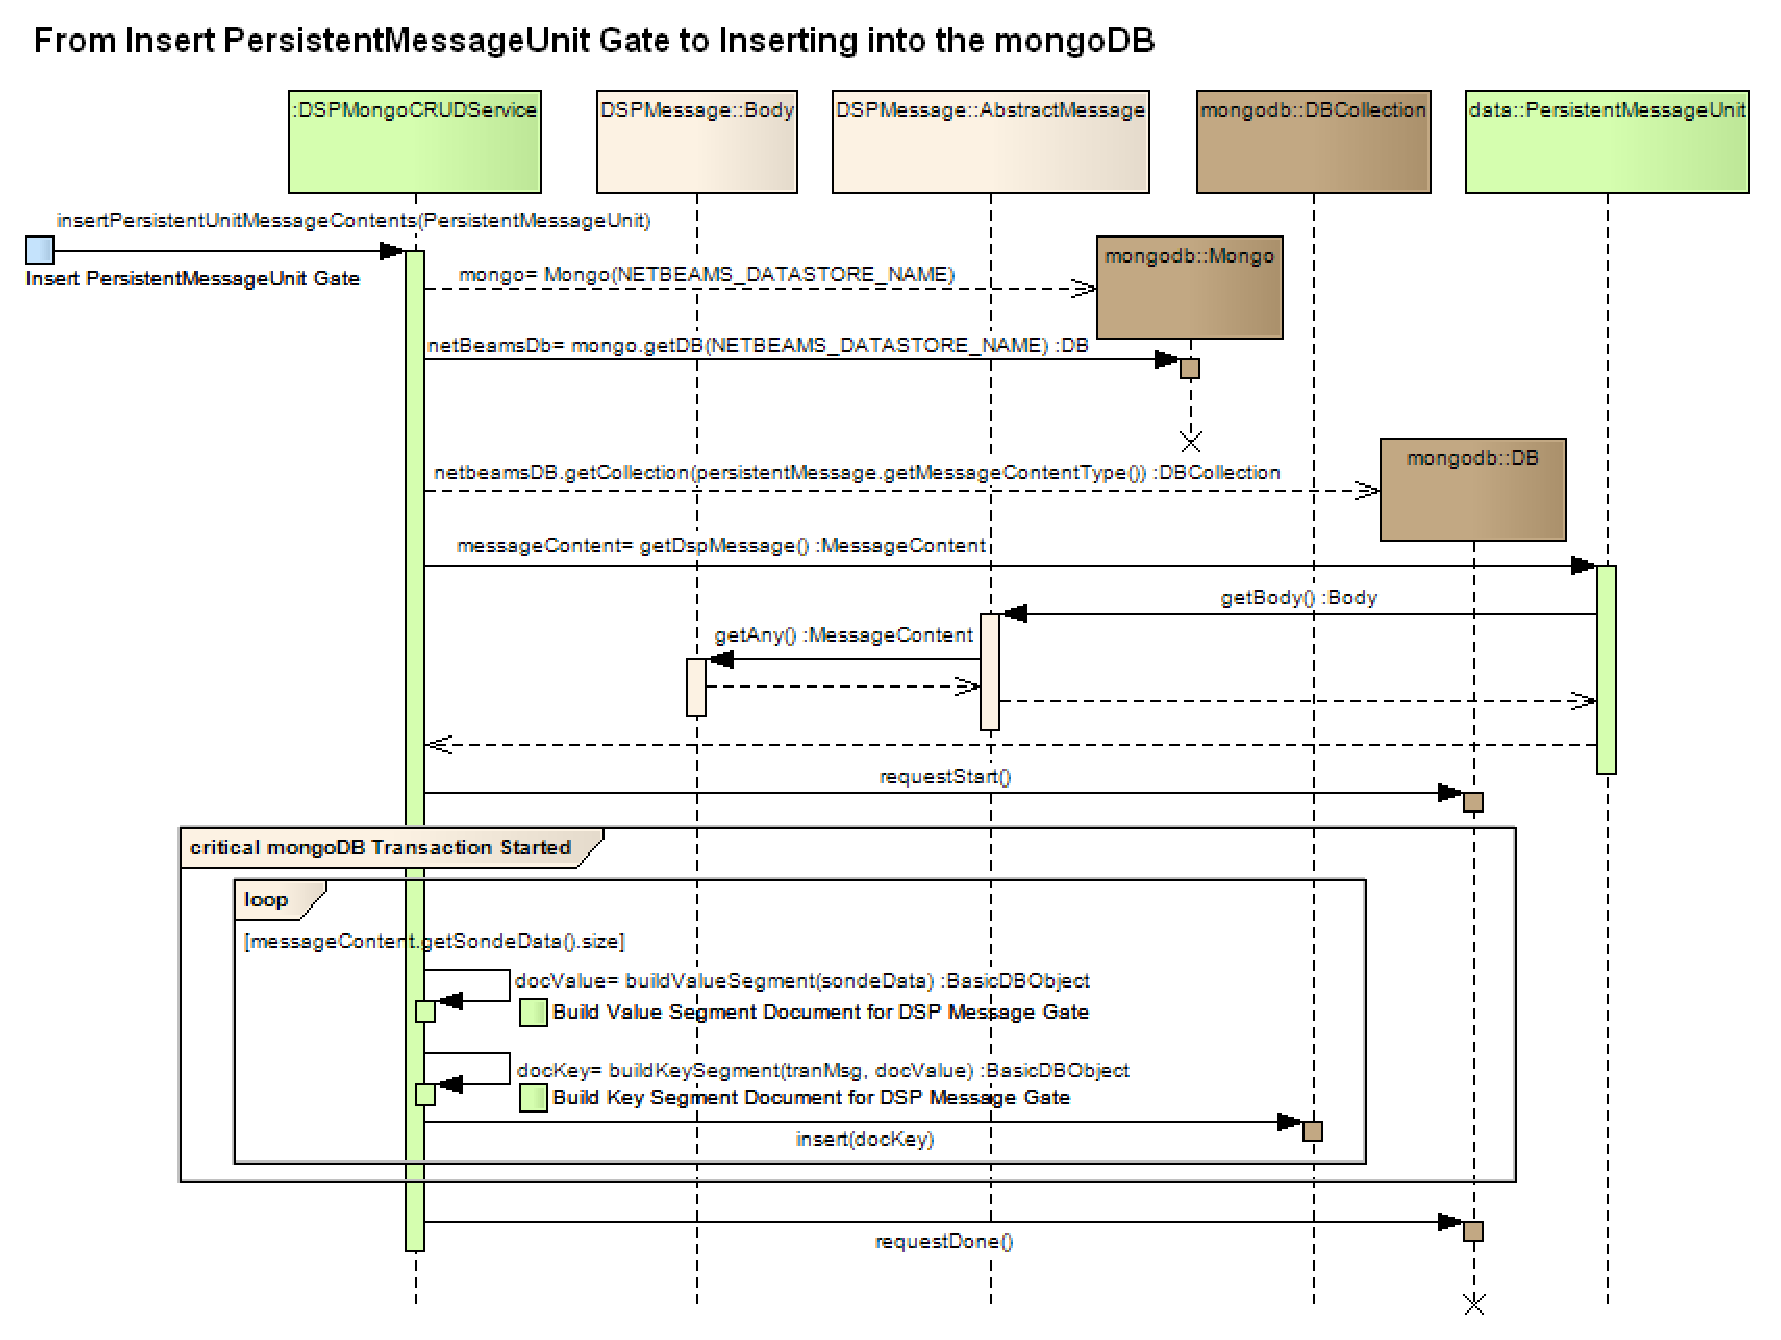
\includegraphics[scale=0.6]{../diagrams/From-Insert-PersistentMessageUnit-to-mongoDB} 
  \caption{UML Sequence Diagram - MessageContent instance saved by the class
  mongoDB service}
  \label{fig:From-Insert-PersistentMessageUnit-to-mongoDB}
\end{figure}

\subsubsection{Creating mongoDB Document instance of Key-Values}

In order to build the document key and value segments, as described in
section \ref{sec:dsp-persistence-data-model}, the reference to the DSP message
is used, as the value key is built by extracting the DSP Message Content from
the body of the DSP Message. Similarly, the key is built by gathering
information from the DSP Message and the PersistenceMessageUnit class. Each of
the properties collected from the YSI Sonde sensor device is collected and
associated with the keys defined for the Value Segment.

\begin{figure}[!h]
  \centering
  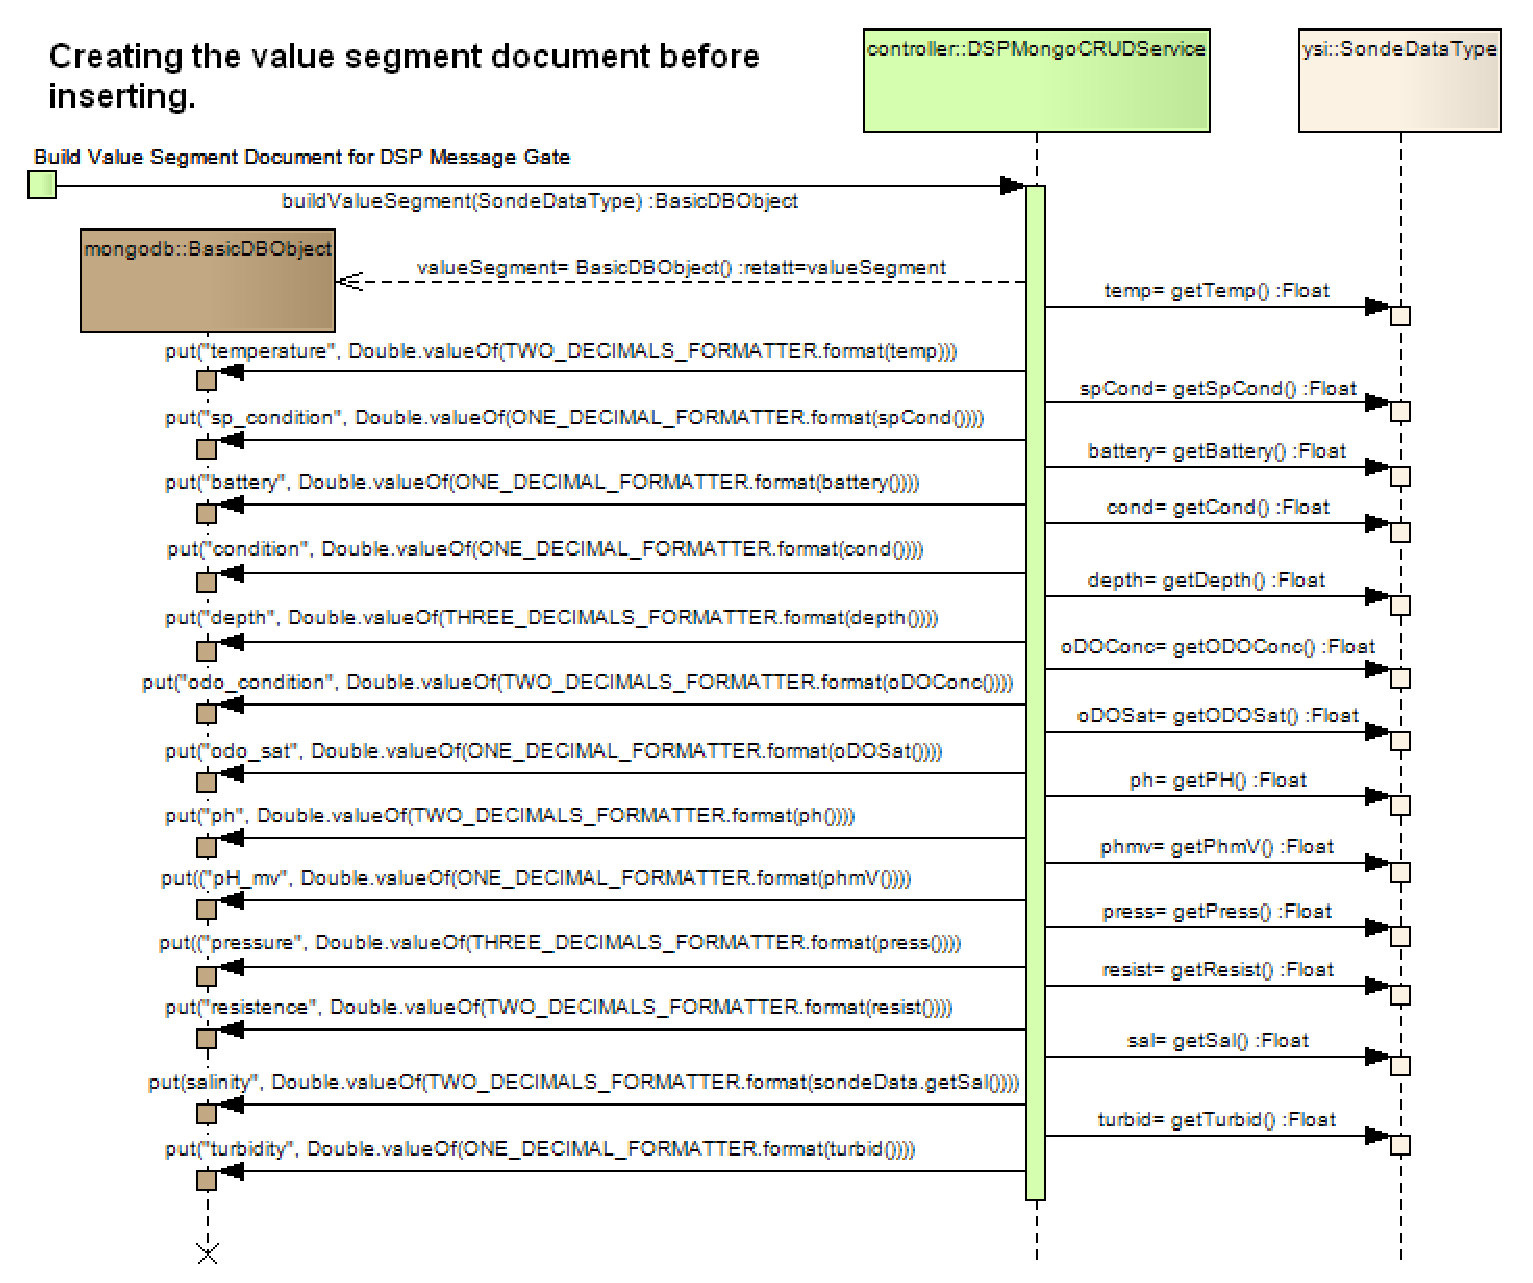
\includegraphics[scale=0.6]{../diagrams/From-Creating-Value-Segment-Sequence}
  \caption{UML Sequence diagram showing the creation of the value document segment}
  \label{fig:From-Creating-Value-Segment-Sequence}
\end{figure}

\newpage

Once the Value Segment is created, the Key Segment is prepared as described in
the UML Sequence Diagram in Figure
\ref{fig:From-Creating-Key-Segment-Sequence}.

\begin{figure}[!h]
  \centering
  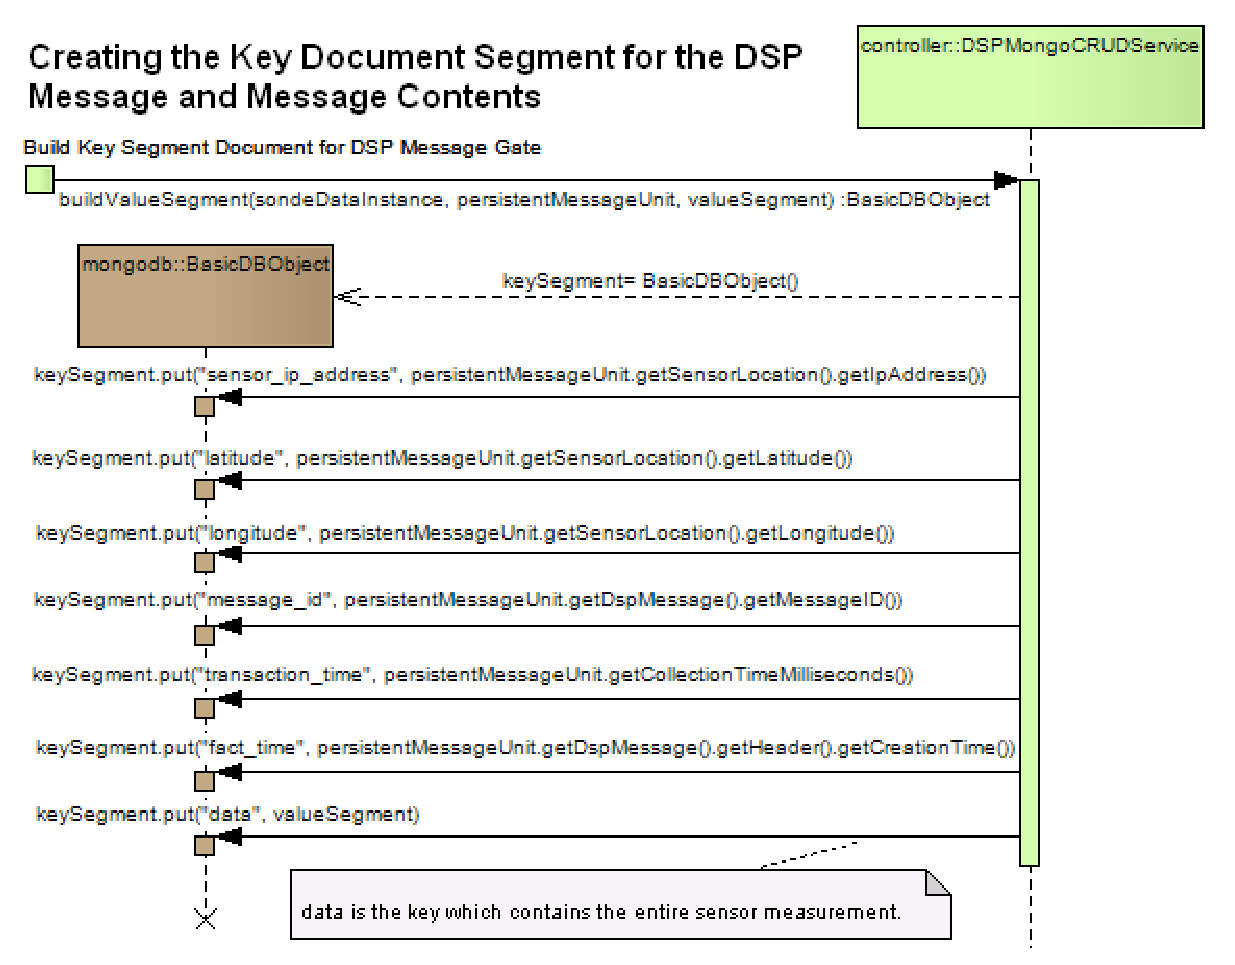
\includegraphics[scale=0.65]{../diagrams/From-Creating-Key-Segment-Sequence}
  \caption{UML Sequence diagram showing the creation of the key document segment}
  \label{fig:From-Creating-Key-Segment-Sequence}
\end{figure}

To Summarize, the DSP Data Persistence Component is added into the DSP Platform
by introducing a new component that provides service to the transfer any
collected data from sensor devices to mongoDB, the Key-Value Pair database
technology. The general dependencies of the system can be seen in UML
Class Diagram depicted by Figure \ref{fig:DSP-Data-Persistence-Classes}, that
expands the UML Package Dependency Diagram shown in Figure
\ref{fig:DSP-Data-Persistence-Packages-Dependency}.

\begin{figure}[!t]
  \centering
  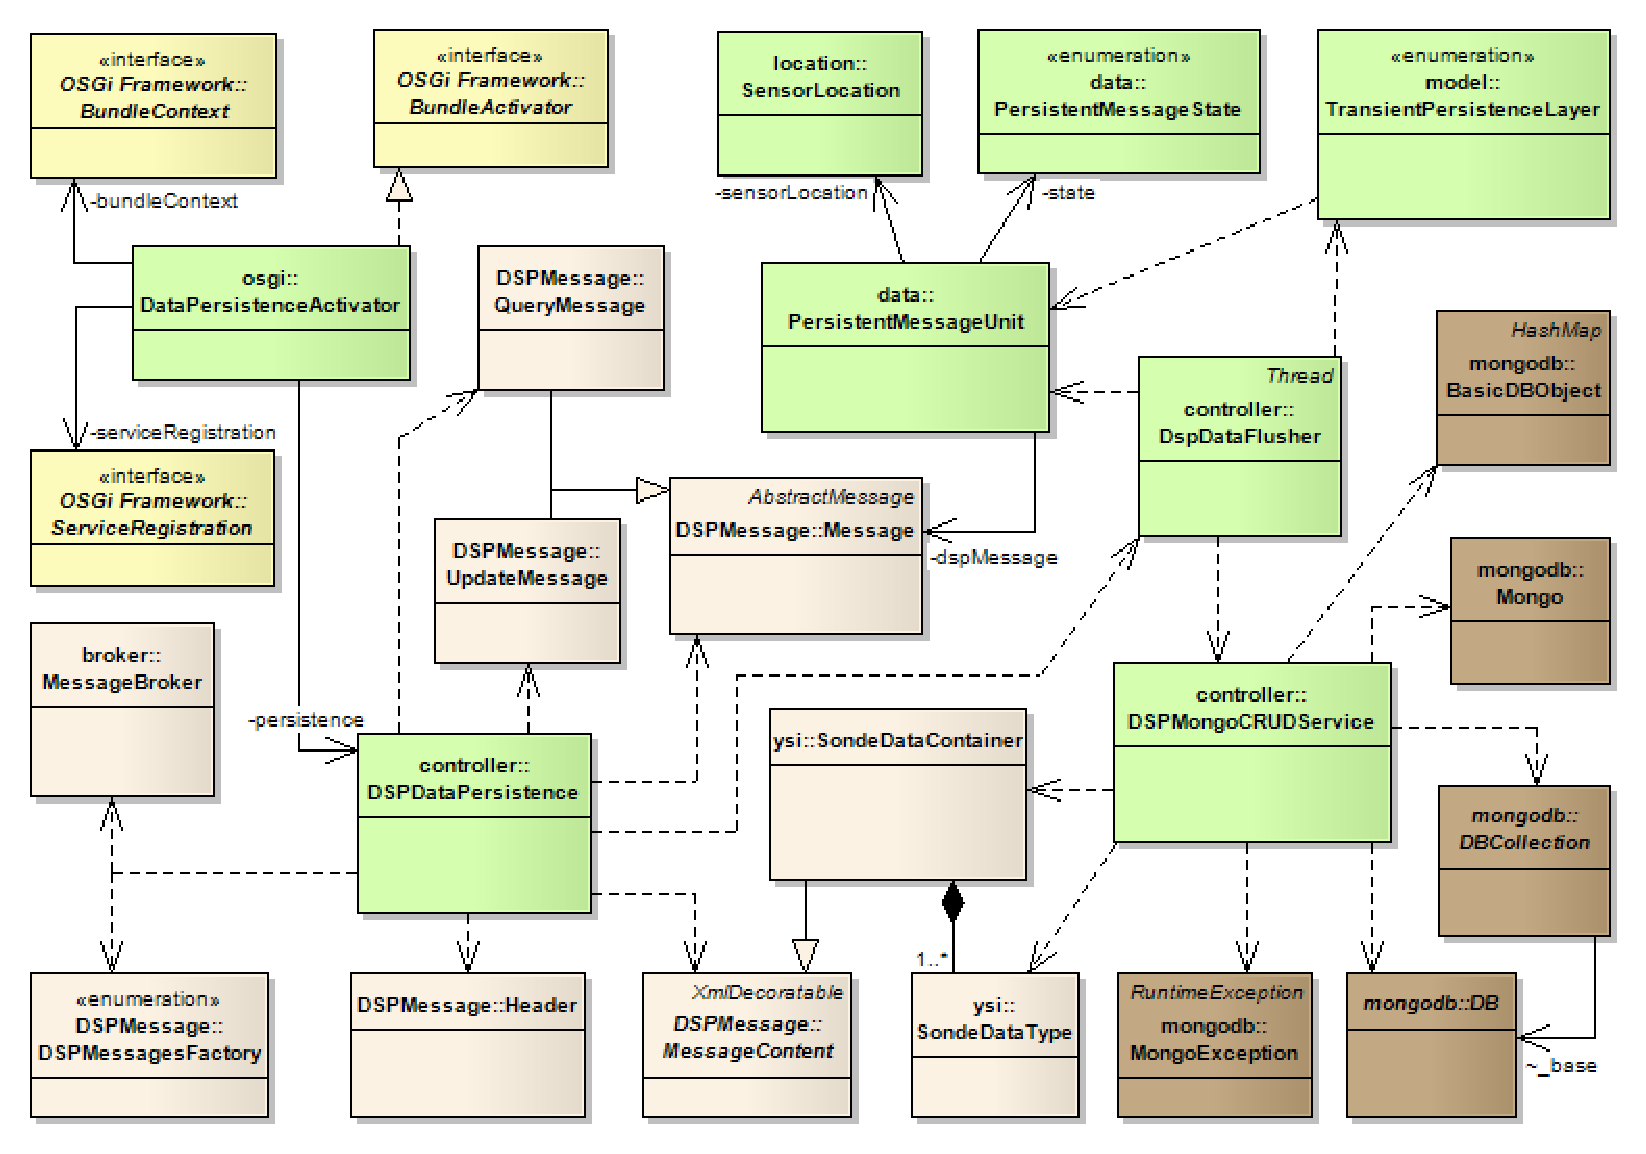
\includegraphics[scale=0.65]{../diagrams/DSP-Data-Persistence-Classes}
  \caption{UML Class diagram for the DSP Data Persistence component.}
  \label{fig:DSP-Data-Persistence-Classes}
\end{figure}

Next section analyzes the deployment details for the DSP Platform and the
mongoDB integration.

\section{DSP Data Persistence Deployment}

The deployment of the persistence layer is accomplished by the addition of two
new components to the DSP Platform: the DSP Data Persistence component and MongoDB
Database Server. The DSP Data Persistence component is responsible for capturing 
any data produced by sensors in the data sink, while mongoDB is where the data is 
going to be stored, as a result of the technology selection on the previous chapter. 

The deployment of the DSP Data Persistence follows the deployment specifications
of a DSP Component over an OSGi Framework. For the development of this work,
the Knopflerfish OSGi Container was used. The details of implementation are described
in section \ref{sec:dsp-data-persistence-implementation}. The deployment of the 
mongoDB can be accomplished in different approaches, summarized as follows: 

\begin{itemize}
  \item \textbf{Single Server}: a regular deployment of a database system as it
  is done in general applications, where data is managed by one single process;
  \item \textbf{Sharded Server}: a deployment approach where data is sharded
  into different servers.
\end{itemize} 

The single server approach maintains all data located in a simple space.
Distributed Systems applications such as Master-Slave, Data Replication, etc
can be used in this approach for scalability
\ref{fig:DSP-Data-Persistence-Deployment-Single}. 

\begin{figure}[!h]
  \centering
  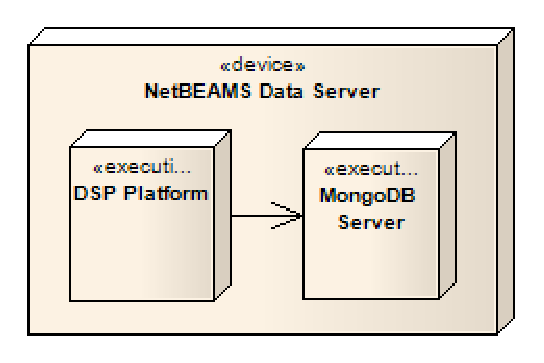
\includegraphics[scale=0.7]{../diagrams/DSP-Data-Persistence-Deployment-Single}
  \caption{UML Deployment diagram with a single server}
  \label{fig:DSP-Data-Persistence-Deployment-Single}
\end{figure}

Given that mongoDB provides support for Database Partitioning by using
the concept of Shards, the implementation of a Data-Centric approach can be done
by deploying different mongoDB instances in a distributed cluster, where each
node can hold different collections of data. mongoDB provides Horizontal
Partition with automatic distribution based on the ranges of a given key of
the document. For NetBEAMS collected data, a good candidate for partitioning is
the time when the data was created, and separate each shard in groups of month
of the year.

\begin{figure}[!h]
  \centering
  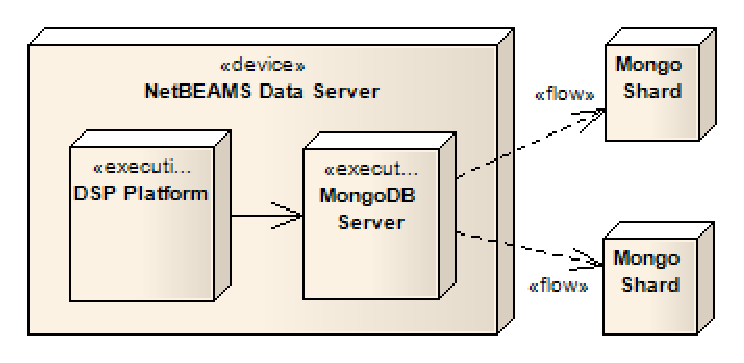
\includegraphics[scale=0.7]{../diagrams/DSP-Data-Persistence-Deployment-Sharded}
  \caption{UML Deployment Diagram for a sharded server}
  \label{fig:DSP-Data-Persistence-Deployment-Sharded}
\end{figure}

The design of the DSP Data Persistence uses the DSP Component specification
defined by the DSP Platform. First, the analysis of the business process
helped to understand the requirements of the system. The data model design
followed the specifications defined in chapter 5. Each of the layers of the
system was described using UML Diagrams, having partial details regarding the
OSGi implementation. The next chapter entails the experiments conducted to
evaluate the designs discussed in this chapter, and walks through the
experiments conducted to verify the implementation of using mongoDB.

%% main.tex, to be used with thesis.tex
% This contains the main work of your thesis.

%\bibliography{thesis}  % uses the references stored in Chapter1Radar.bib

\chapter{DSP Data Persistence: Component Implementation}

This section shows the implementation of the DSP Data Persistence, which
follows the specifications of the DSP Components described on section 2.4,
along with the setup of the mongoDB, the chosen database system that handles
document-oriented instances. The implementation of the DSP Data Persistence
component was developed using the DSP Subversion repository at
http://code.google.com/p/netbeams.

\section{DSP Deployment on OSGi Framework}

    * Description of the OSGi MANIFEST.MF
    * Description of the component on the config.xml
    * Adding a matching rule on the matcher\underline{ }config.xml
    * Adding a bootstrap message the component and database configuration


    * Adding a new entry into the deployment configuration artifact config.xml;
    * Adding a new entry into the matcher configuration artifact matcher\underline{ }config.xml;
    * Adding an optional configuration message that sets up the new DSP Component;
    * Adding new Java drivers that communicates with the Database system;
    * Installing and configuring the proposed database system.

\subsection{Starting the DSP Platform}

    * command-line (Knopflerfish Framework)
    * user interface (Knopflerfish Framework)

\subsection{Stopping the the DSP Platform}

    * command-line (Knopflerfish Framework)
    * user interface (Knopflerfish Framework)

\subsection{Execution Logs}

\section{mongoDB Deployment}

Given that Document-Oriented Model makes a good candidate persist sensors'
properties and the recently enumerated list technologies in the previous
article DSPDataPersistence, the open-source project called mongoDB was chosen
for the evaluation on our case study, the netBEAMS DSP Platform.

mongoDB supports storage based on collections of data, stored using BSON, a
binary representation the JSON data representation format, including dynamic
queries and indexing support. As it's stated in their web site, mongoDB
"bridges the gap between key/value stores (which are fast and highly scalable)
and traditional RDBMS systems (which are deep in functionality)".

\begin{itemize}
  \item mongoDB implements a document-oriented structure, which is similar to
  KVP;
  \item mongoDB is written in C++, and therefore, can is available in any major
  platform, as well as offers a broad range of API drivers written in different
  languages such as Java, Python, Perl and Ruby; 
  \item mongoDB is open-source, with good community support and availability
  through mailing lists, freenode IRC channel, and commercial support through
  10gen company; 
  \item mongoDB has support to distributed systems properties such as
  Master-Slave replication, and features like Database Shards with
  auto-sharding based on shard keys.
\end{itemize} 

nstallation of mongoDB
- Explanation about mongoDB processes: mongod, mongos, mongo
- Specification of the shards, shard key, etc

    * The database instance is called "netbeams";
    * The database "netbeams" may contain different collections, categorized by
    the Sensor Content Type, that is, depending on how the DSP Component was
    described;  

\subsection{Document-Oriented Data Model}

An example of the data is as folows (using the JSON syntax). Listing
\ref{file:mongodb-ysi-data-format} follows the strategy described on Section X,
where the entity representation is denormalized, and each of the properties of
the sensor is repeated in each instance of the data. The fact and transaction
times are expressed in milliseconds. The data element contains the complete
structure of the originating sensor such as the IP address. The collection of
instances of this document represents the sensor data type.

\subsection{Starting the Database}

\subsection{Stopping the Database}

\subsection{Execution Logs}

- Java API implementation
- Python API implementation

\section{Data Access Using Database Shell}

The mongoDB client can be started by using the following command. Make sure you
have started the mongoDB server before executing the mongoDB client.

mongo netbeams | tee output\underline{ }number\underline{ }date.log

Here, the iterative mongo client shell offers users to verify and navigate on a
given database and its collections. This first section shows the connection of
the mongo client to the database netbeams. It also highlights the query for the
collections available. During the experiment, the SondeDataContainer?
collection was created as related to the type from the DSP Messages for the YSI
Sonde.

The shell references to the mongoDB system can be found at
http://www.mongodb.org/display/DOCS/dbshell+Reference 

\lstset{label=cmd:mongo,caption=Execution of mongo client}
\begin{lstlisting}
MongoDB shell version: 1.1.0-
url: netbeams
connecting to: netbeams
type "help" for help
> show collections
SondeDataContainer
system.indexes
>
> db.SondeDataContainer.count()
1000000
\end{lstlisting}

Then, the first verification of the data integrity is regarding the number of
elements created. Here, the first count() function on the collection returned
1000000.

An example about retrieving the first element of the collection can be done
using the findOne() function. It will return an element instance on the
JSONnotation.

\lstset{label=cmd:mongo-findone,caption=Querying the database: one item}
\begin{lstlisting}
> db.SondeDataContainer.findOne()
{"_id" :  ObjectId( "d36f4007b7e7ac4a03c60000")  , "sensor_ip_address" : "192.168.0.136" , "message_id" : "7b6624d6-0ca1-4cba-a343-f166e88da73b" ,
"transaction_time" : 1252845473412 , "fact_time" : 1252845346000 , "data" : {"temperature" : "45.01" , "sp_condition" : "37.6"
, "condition" : "145.8" , "resistence" : "159.77" , "salinitude" : "0.0" , "pressure" : "0.391" , "depth" : "0.46" , "ph" : "5.64" ,
"pH_mv" : "-62.1" , "odo_sat" : "89.7" , "odo_condition" : "59.34" , "turbidity" : "0.0" , "battery" : "9.4"}}
\end{lstlisting}

The query based on attributes can be done using the "dot" notation, as you
navigate through the JSON documents. Additionally, you can use the functions as
aggregated on the result of others. The example in listing
\ref{cmd:mongo-find-list} counts the number of documents with the key
"data.ph" equals to "5.64".

\lstset{label=cmd:mongo-find-list,caption=Execution of mongo client}
\begin{lstlisting}
> db.SondeDataContainer.find({"data.ph":5.64)}).count()
1226
\end{lstlisting}

The following example is the output of the first 2 documents from the same
previous query using the limit() function, as shown in figure
\ref{cmd:mongo-find-limit}.

\lstset{label=cmd:mongo-find-limit,caption=Query Element with specific
projection limiting the result set size}
\begin{lstlisting}
> db.SondeDataContainer.find({"data.ph":5.64}).limit(2)
{"_id" :  ObjectId( "d36f4007b7e7ac4a03c60000")  , "sensor_ip_address" : "192.168.0.136" , "message_id" : "7b6624d6-0ca1-4cba-a343-f166e88da73b"
, "transaction_time" : 1252845473412 , "fact_time" : 1252845346000 , "data" : {"temperature" : "45.01" , "sp_condition" : "37.6" ,
"condition" : "145.8" , "resistence" : "159.77" , "salinitude" : "0.0" , "pressure" : "0.391" , "depth" : "0.46" , "ph" : "5.64" ,
"pH_mv" : "-62.1" , "odo_sat" : "89.7" , "odo_condition" : "59.34" , "turbidity" : "0.0" , "battery" : "9.4"}}
{"_id" :  ObjectId( "d36f4007b7e7ac4a1fc80000")  , "sensor_ip_address" : "192.168.0.136" , "message_id" : "7b6624d6-0ca1-4cba-a343-f166e88da73b" ,
"transaction_time" : 1252845473412 , "fact_time" : 1252845346000 , "data" : {"temperature" : "46.71" , "sp_condition" : "60.8" ,
"condition" : "160.6" , "resistence" : "1399.4" , "salinitude" : "0.01" , "pressure" : "1.057" , "depth" : "2.485" , "ph" : "5.64" ,
"pH_mv" : "-16.3" , "odo_sat" : "58.8" , "odo_condition" : "19.29" , "turbidity" : "0.2" , "battery" : "9.2"}}
>
\end{lstlisting}

Other logs are located at
http://code.google.com/p/netbeams/downloads/list

\section{Data Access Using APIs}

The mongoDB server offers different drivers to access the data, as well as the
Web Services.

\begin{itemize}
  \item The Java tutorial on the drivers is located at
    http://www.mongodb.org/display/DOCS/Java+Tutorial. The driver is located on
    the NETBEAMS/versions/v2/thirdparty/mongodb directory;  
  \item The REST API can be called from any HTTP client. At the time of the
  editing, this feature is still under alpha version. Check the documentation
  athttp://www.mongodb.org/display/DOCS/Http+Interface for details 
\end{itemize}

The following HTTP GET Request method returns the first 5 documents in the collection:
http://127.0.0.1:28017/netbeams/SondeDataContainer/?limit=-5, as shown in
listing \ref{cmd:mongo-rest-request}.

\lstset{label=cmd:mongo-rest-request,caption=REST HTTP GET Request Example}
\begin{lstlisting}
HTTP/1.0 200 OK
x-action:
x-ns: netbeams.SondeDataContainer
Content-Type: text/plain;charset=utf-8

{
  "offset" : 0,
  "rows": [
    { "_id" : "156f4007e4c3b74a36ed3100", "sensor_ip_address" : "192.168.0.117", "message_id" : "08b02c08-9290-4517-9a28-c6ee7e16509a",
"transaction_time" : 1253557219486, "fact_time" : 1253557217000, "data" : { "temperature" : "31.44", "sp_condition" : "99.8", "condition" : "53.5",
"resistence" : "1157.08", "salinity" : "0.0", "pressure" : "1.066", "depth" : "0.161", "ph" : "1.08", "pH_mv" : "-82.0", "odo_sat" : "40.3",
"odo_condition" : "56.85", "turbidity" : "0.2", "battery" : "8.2" } } ,
    { "_id" : "156f4007e5c3b74a37ed3100", "sensor_ip_address" : "192.168.0.117", "message_id" : "08b02c08-9290-4517-9a28-c6ee7e16509a",
"transaction_time" : 1253557219486, "fact_time" : 1253557217000, "data" : { "temperature" : "37.83", "sp_condition" : "176.3", "condition" : "2.6",
"resistence" : "1324.97", "salinity" : "0.01", "pressure" : "1.36", "depth" : "1.564", "ph" : "0.12", "pH_mv" : "-23.5", "odo_sat" : "104.5",
"odo_condition" : "19.44", "turbidity" : "0.1", "battery" : "5.0" } } ,
    { "_id" : "156f4007e5c3b74a38ed3100", "sensor_ip_address" : "192.168.0.117", "message_id" : "08b02c08-9290-4517-9a28-c6ee7e16509a",
"transaction_time" : 1253557219486, "fact_time" : 1253557217000, "data" : { "temperature" : "74.3", "sp_condition" : "84.0", "condition" : "104.7",
"resistence" : "4089.13", "salinity" : "0.01", "pressure" : "1.222", "depth" : "2.788", "ph" : "6.56", "pH_mv" : "-78.1", "odo_sat" : "40.0",
"odo_condition" : "6.02", "turbidity" : "0.3", "battery" : "3.2" } },
  "total_rows" : 3 ,
  "query" : {} ,
  "millis" : 0
}
\end{lstlisting}

Data visualisation tools for mongoDB is slowly being developed by open-source
developers. The next picture shows the database "netbeams" and the collection
"SondeDataContainer  ?" being rendered by futon4mongodb, one of the
open-source tools developed to visualise mongoDB data.

\section{Visualizing Data on The Browser}

Futon4Mongo is an open-source software adapted from CouchDB \ref{couchdb}.
First, the collections list is shown. Figure
\ref{fig:view-collections-instance-browser-futondb} shows one single collection
for the YSI data containing 1 million objects.

\begin{figure}[h]
  \centering
  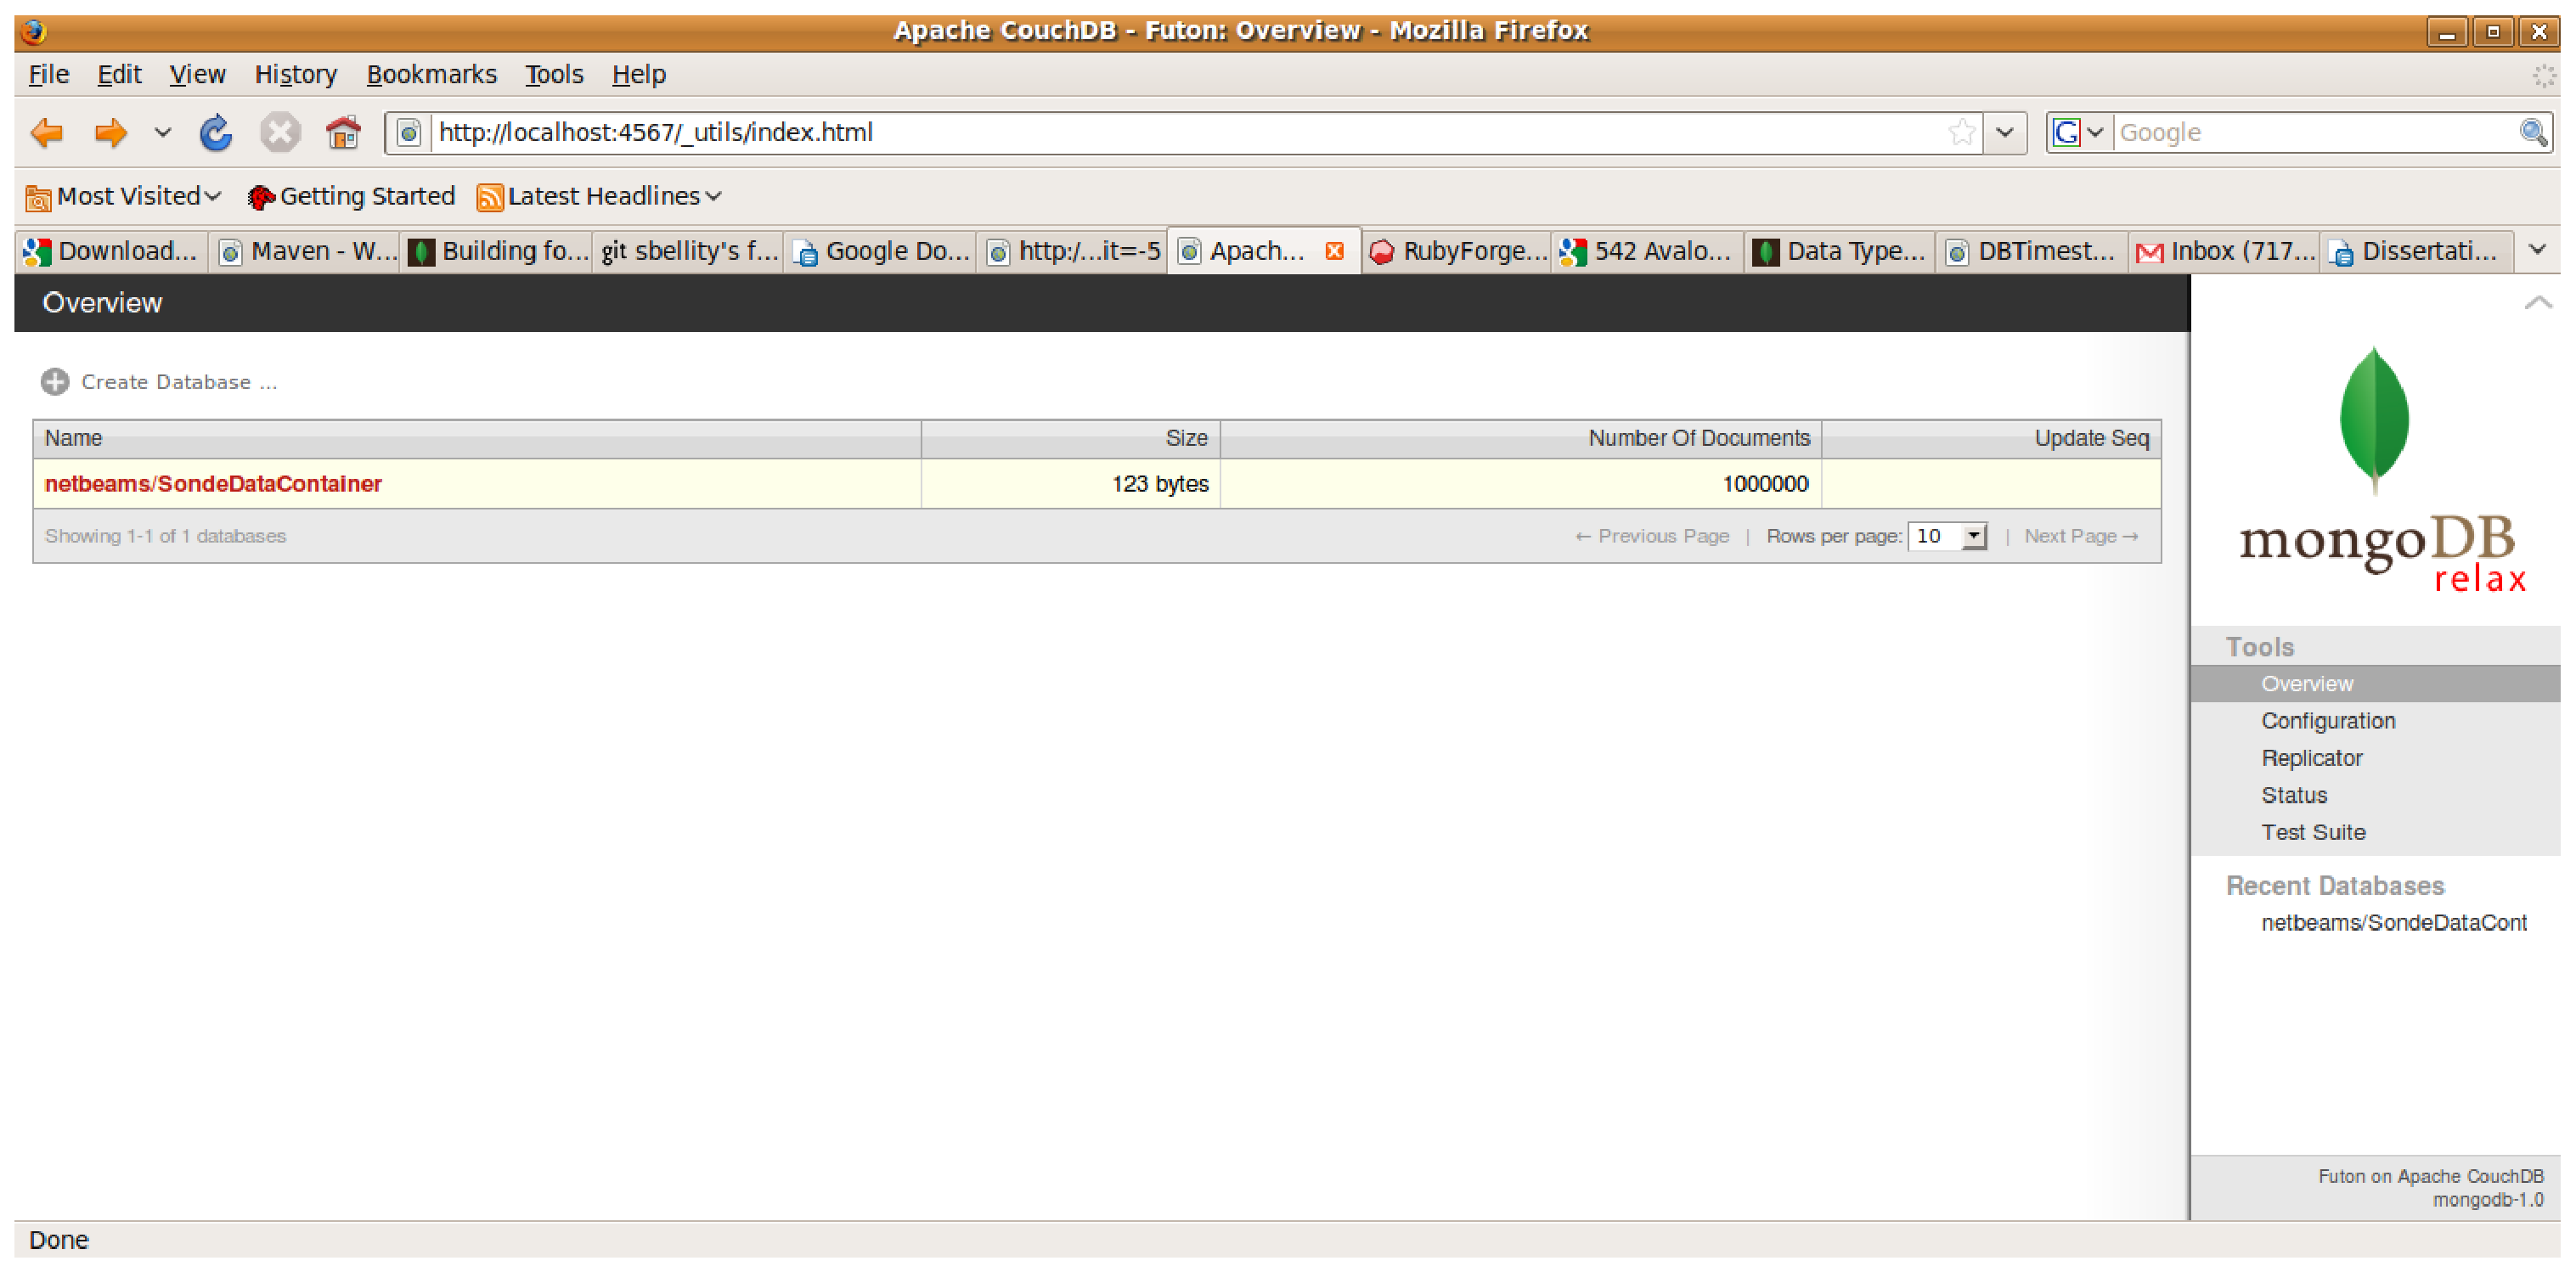
\includegraphics[scale=0.3]{../diagrams/view-collections-instance-browser-futondb}
  \caption{Viewing a partial list of data using the Futon for CouchDB/MongoDB}
  \label{fig:view-collections-instance-browser-futondb}
\end{figure}

The collection is composed by instances of documents of representing the YSI
Sonde type, being indexed by a document ID and the values being the keys
defined in the previous chapter, as shown in figure
\ref{fig:view-collected-data-list-browser-futondb}.

\begin{figure}[h]
  \centering
  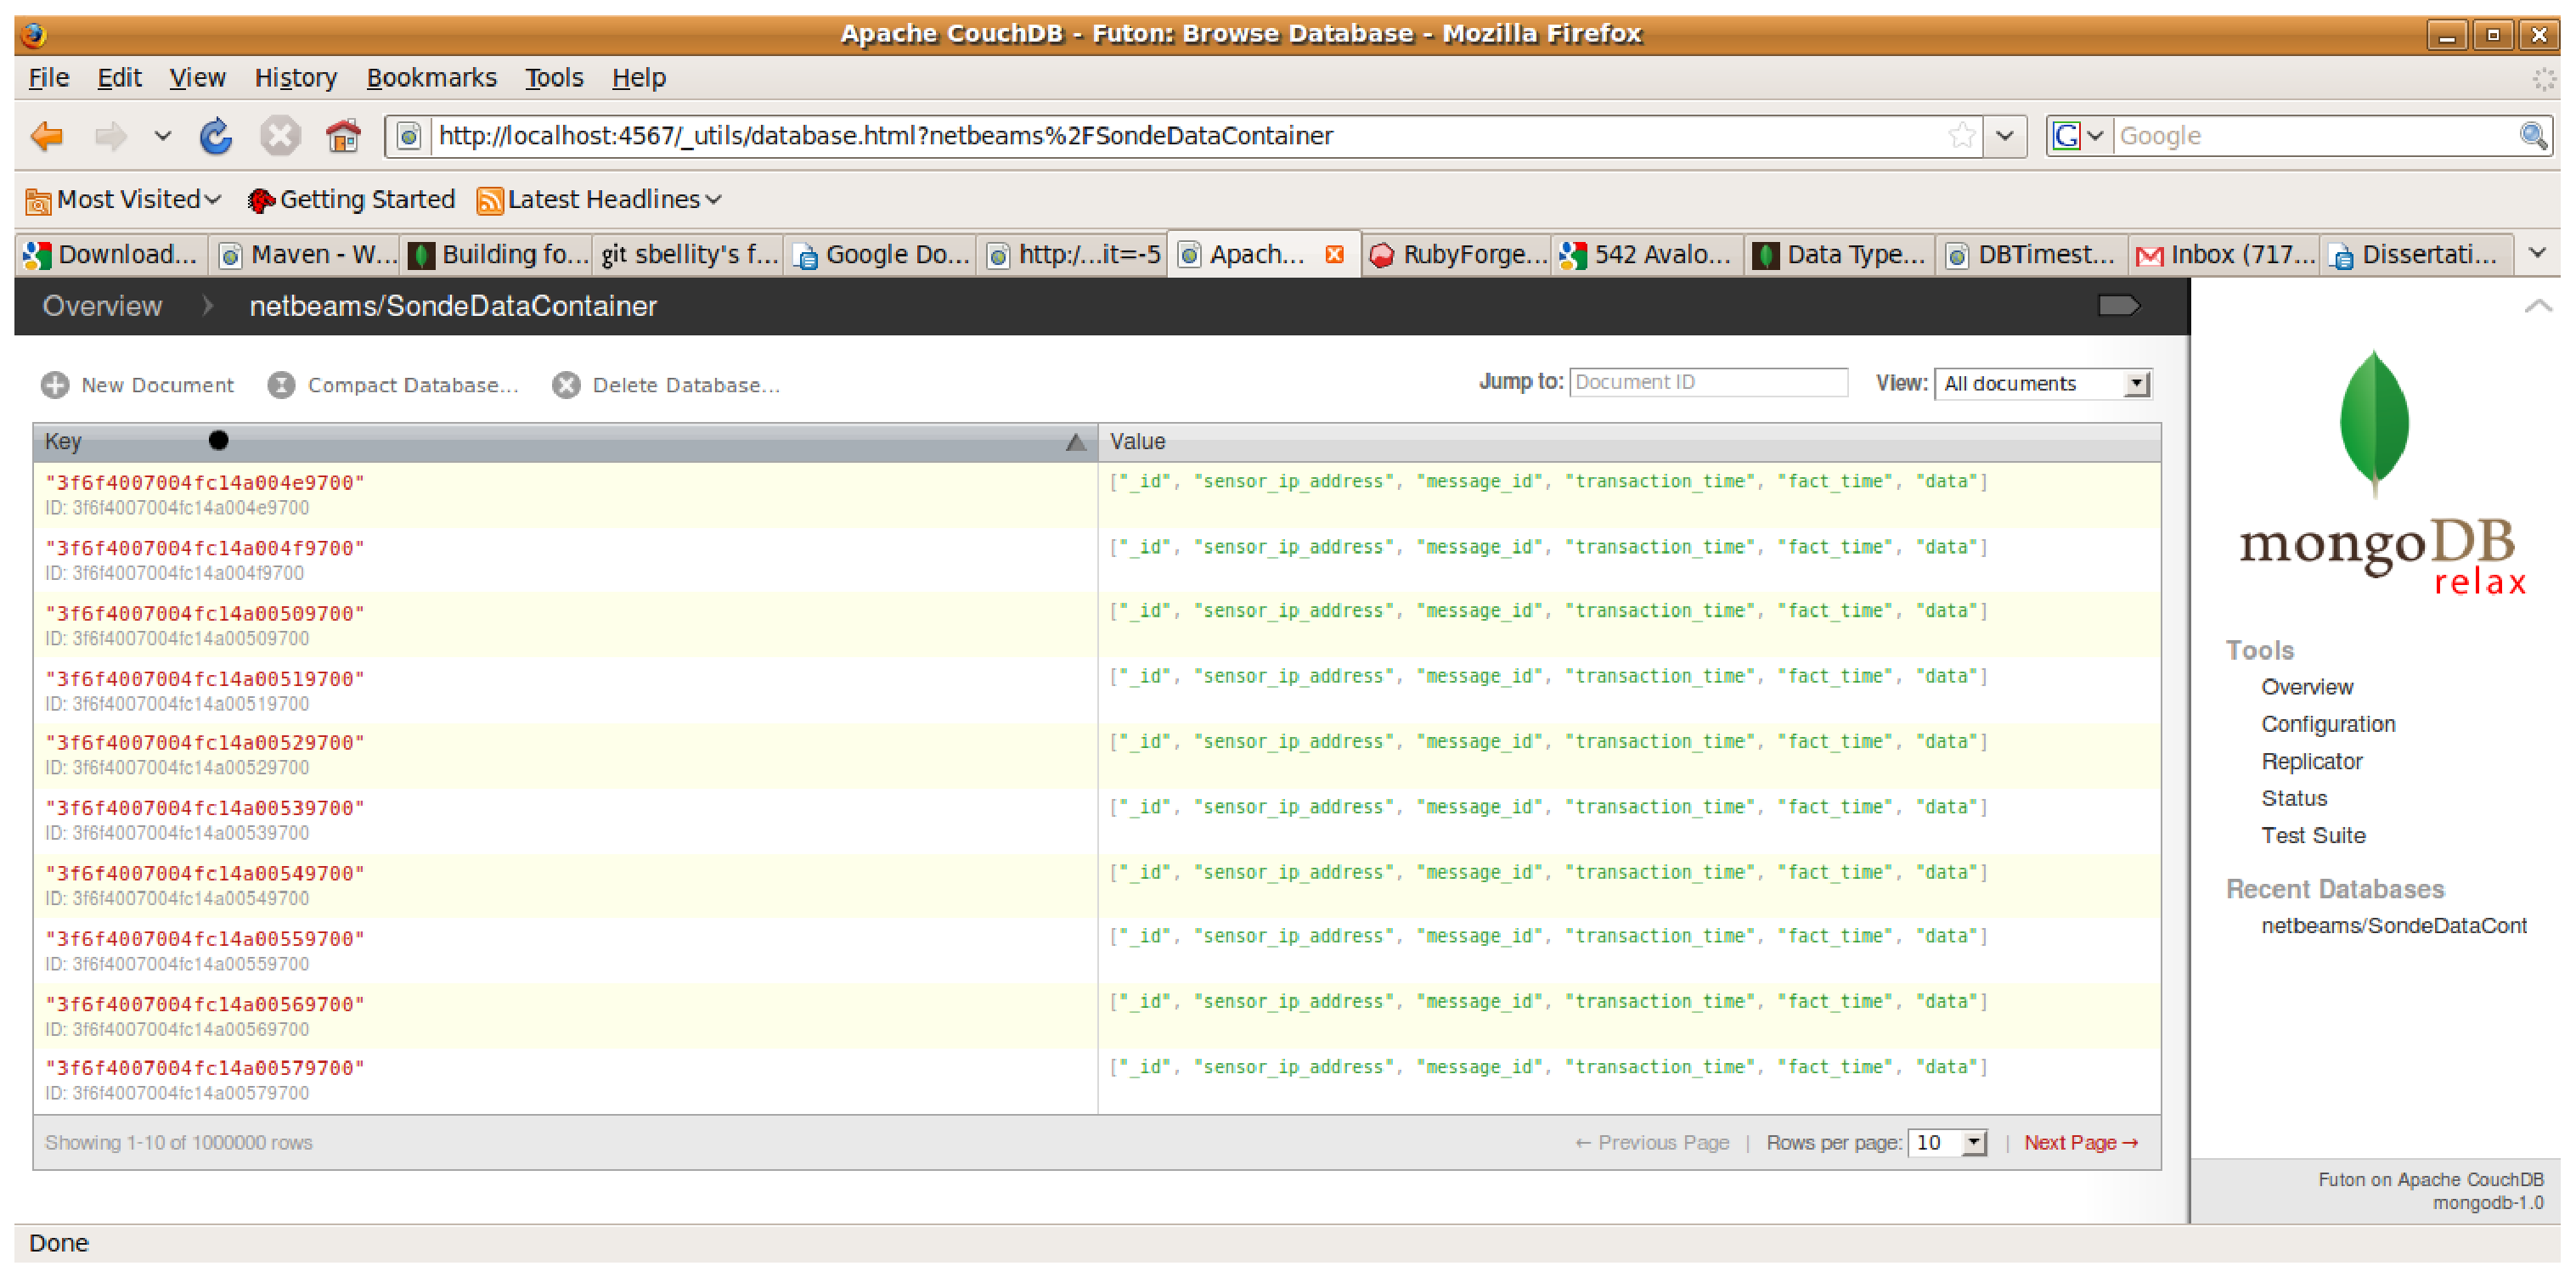
\includegraphics[scale=0.3]{../diagrams/view-collected-data-list-browser-futondb}
  \caption{Viewing a partial list of data using the Futon for CouchDB/MongoDB}
  \label{fig:view-collected-data-list-browser-futondb}
\end{figure}

By clicking in one of the items, one can view the instance of the document, as
it is shown in figure \ref{fig:view-collections-instance-browser-futondb}.

\begin{figure}[h]
  \centering
  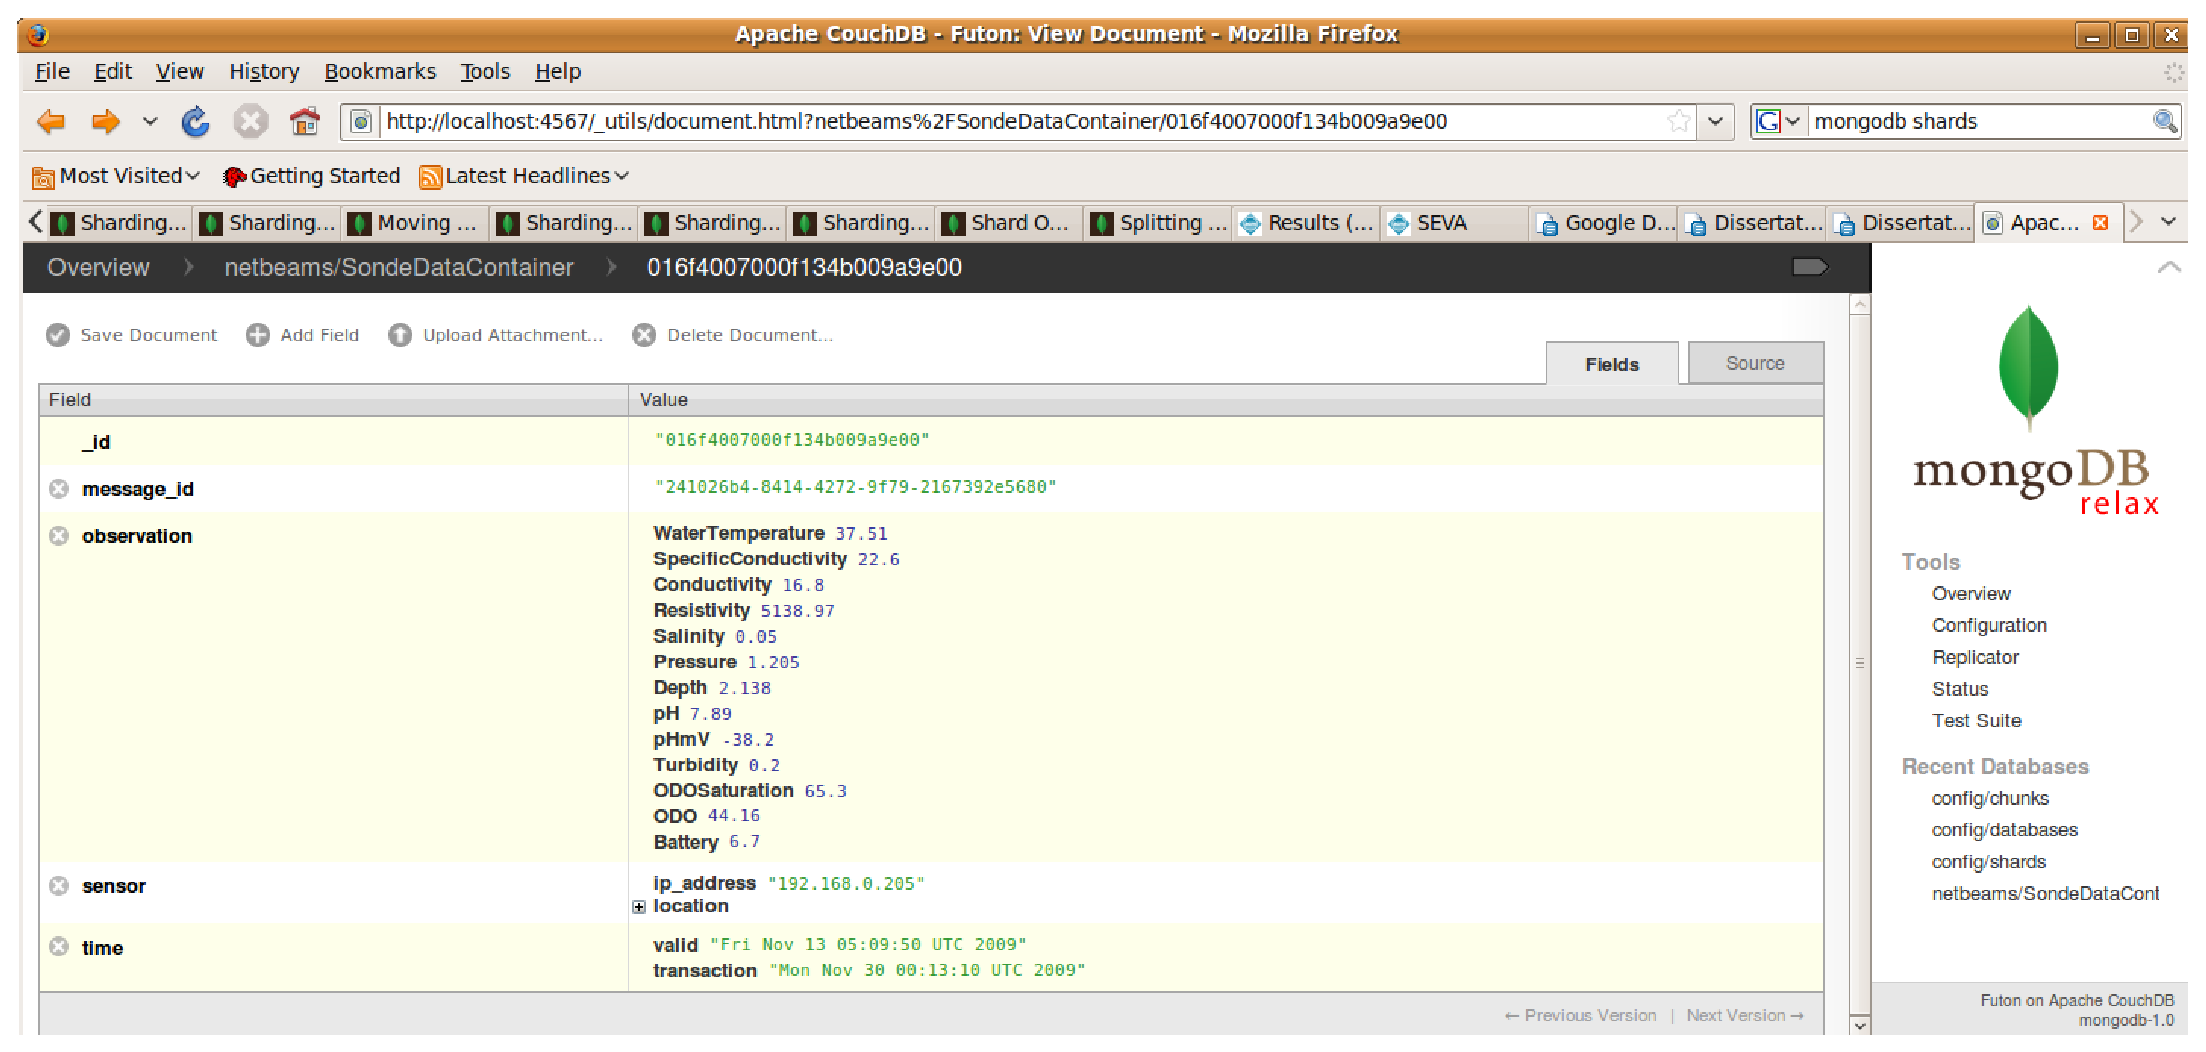
\includegraphics[scale=0.3]{../diagrams/view-collected-data-instance-browser-futondb}
  \caption{Viewing an instance of collected data using the Futon for
  CouchDB/MongoDB}
  \label{fig:view-collected-data-instance-browser-futondb}
\end{figure}

\section{Exporting Data to Spreadsheets}

mongoDB has an export facility shell called mongoexport. It can export the data
in JSON format or CSV. One may also write its own export tool in any of the
languages such as Java, PHP, Python, Perl, Ruby, among others. A list of the
existing drivers in different languages is provided
athttp://www.mongodb.org/display/DOCS/Drivers. The following command can be
executed to have the exported version of the data in CSV (read the help output
of the command for details).

An example to export the data in CSV format can be seen in listing
\ref{cmd:mongoexport}, and an example containing 1 million objects can be
downloaded at
http://netbeams.googlecode.com/files/experiment-1000000-data-exported-20090913-053538.csv.tar.gz.

\lstset{label=cmd:mongoexport,caption=Command to export data in CSV format}
\begin{lstlisting}
mongoexport -d netbeams -c SondeDataContainer --dbpath ./data/ --csv -f "_id,sensor_ip_address,transaction_time,fact_time,
data.temperature,data.sp_condition,data.condition,data.resistence,data.salinitude,data.pressure,data.depth,data.ph,data.pH_mv,data.odo_sat,
data.odo_condition,data.turbidity,data.battery" -o sonde-data-exported.csv
\end{lstlisting}

\section{Exporting Data to OPeNDAP Format}

By using any programming language driver, one can export data in the OPeNDAP
format.
% main.tex, to be used with thesis.tex
% This contains the main work of your thesis.

%\bibliography{thesis}  % uses the references stored in Chapter1Radar.bib

\chapter{Experimental Results: Correct Behavior and Performance}

As discussed in the previous chapter, the implementation of a data persistence
layer for NetBEAMS followed the requirements defined in chapter 4 having in
mind the classification of the SF-BEAMS sensor network and the software
infrastructure provided by the Data Sensor Platform. As a result, the
implementation was developed using the infrastructure provided by the online
version-control system repository from NetBEAMS, whose documentation is
detailed in section \ref{sec:dsp-data-persistence-implementation}.

First, this chapter details the experiment setup designed to evaluate the
proposed implementation, showing the measurement results collected from the
simulation log and based on the user experience while reusing the collected
data. Last, but not least, the pertinent discussion of this work is devided up
into different sections, each of them analyzing different aspects related to
data persistence for NetBEAMS, amongo others.

\section{Experiment Setup}

The experiment was designed to support different scenarios of a regular use of
the mongoDB system infrastructure, simulating the activities of data collection
from the SF-BEAMS network using the NetBEAMS infrastructure. First, the setup
for the data collection of randomly generated data was implemented, which
directly uses NetBEAMS already existing classes. Then, the implementation of
the CRUD scenarios were implemented in different programming languages, from
the data insertion scenario using the Java Programming Language, and then the
remaining operations using the Javascript Scripting language \cite{javascript}
and the Python Programming Language \cite{python}. Similarly, an open-source web
application, developed in the Ruby Programming language \cite{ruby}, was also
used. The experiment scripts were writen using Shell Bash Script Language
\cite{bashshell} and is responsible for orchestrasting the execution of one
single experiment ``run''.

\subsection{Experiments Artifacts}

Different artifacts were created to perform the different experiments
operations. The Create function was developed in Java, without the interversion
of the DSP or OSGi, isolating only the functionalities of provided by CRUD
service class DSPMongoCRUDService (Listing \ref{file:dsp-mongo-service}),
responsible for the connection handling with mongoDB, as well as the insertion
operation from NetBEAMS. As described in section \ref{sec:dsp-details}, the
current version of NetBEAMS supports the data collection for the YSI Sonde
device, among others used for demo purposes such as a software sensor that
captures the mouse activities over a window. The documentation of both data
types is seen in section \ref{sec:dsp-payload-implementation}. In this way, the
DSP Data Persistence, as described in the previous section, supports both data
types to be persisted.

In order to exercise mongoDB with the same data collected from NetBEAMS, the
existing Java class TestSondeData (Listing
\ref{file:random-ysi-data-generator}), was refactored to provide a random
instance generator for the YSI Data handler implemented in the Java class
SondeDataType (Listing \ref{file:main-ysi-data-handler}). When the Insert
function is executed, the created instances are transferred from the JVM to
the mongoDB, and stored in the collection ``SondeDataContainer''. Specific
details about the execution of mongoDB are depicted in section
\ref{sec:mongodb-deployment}. Finally, the implementation of the experiment
in the Java class DSPMessageToMongoDBExperiment (Listing
\ref{file:experiment-dsp-java-executor}) was responsible for managing the
creation and insertion of any workload composed by instances of the class
SondeDataType in a bulk manner.

Similarly, the support for the Retrieve, Update and Delete operations against
the inserted workload were implemented using Javascript, as shown in Listing
\ref{file:experiment-scenarios}, respectively by the function calls ``find'',
``update'' and ``remove'' over the collection ``SondeDataContainer''.
Similarly, in order to implement a customizable export system that converts
from mongoDB into the format OpenDAP, a simpler prototype script was developed
in Python, as shown in Listing \ref{file:experiment-export-python}. As a result
of the execution of this script, the exported artifact has the same format as
described in Listing \ref{file:rtc-ysi-opendap}. 

On the other hand, the execution of the main experiment shell script requires
the use to provide the size of the workload, as shown in listing
\ref{cmd:run-persistence-experiment}.

\lstset{label=cmd:run-persistence-experiment,caption=Running main experiment
shell script}
\begin{lstlisting}
marcello@netbeams-dev:~/workspaces/netbeams/versions/v2/persistence$ ./run-persistence-experiment 
#######  NetBEAMS Experiments - Persistence on MongoDB  ########

Usage: ./run-persistence-experiment X, where X is the size of the workload to be inserted from NetBEAMS YSI Data Handler to mongoDB
\end{lstlisting}

\subsection{Used Workload}
\label{sec:workload}

The workload selected for the experiments reflects the current use of the data
at the SF-BEAMS infrastructure. In this way, the experiment runs for 5
different times performed to investigate different scenarios to be described.
In this way, this number is related to the total number of sensor devices
reported to be in operation, as discussed in section \ref{sec:sfbeams}. In
summary, the volume of the workload prepared after the experiment setup
is as follows:

\begin{itemize}
  \item \textbf{First Round}: 483,840 documents, worth the production of the 
  YSI Sonde device during one year, at the rate of 1 observation per minute;
  \item \textbf{Next Rounds}: 483,840 * 4, or 2,419,200 documents, representing
  5 different YSI devices similar to the first round.
\end{itemize}

\subsection{System Environment}

Two different system environments were prepared: one for the External Storage
environment, or Single Server; and another for the Data-Centric Storage, or
Distributed Server. Since the single server is a regular centralized database
system, mongoDB just requires the execution of the database process ``mongod'',
which is started by specifying the directory where the inserted data will be
managed. On the other hand, nonetheless, the distributed server setup requires
a different list of processes (see section \ref{sec:mongodb-user-experience}):
one ``mongod'' process for each mongoDB shard running on the different mongoDB
cluster, one ``mongod'' process to manage the cluster metadata, and one
``mongos'' process, which is the main one responsible to orchestrate the
cluster. In conclusion, the single system environment is synmmetric to
the External Storage used to persist the collected data, while the clustered one
is simulates the Data-Centric Storage one.

The simulation of both the single and distributed system used both a Mac OS 10
Snow Leopard 64bit, with a total of 8GB of physical memory. However, in order
to simulate different shards in different machines, the use of a VirtualBox
\cite{virtualization} provided the use of guest operating systems to run and
act as the mongoDB shards. In this way, two different versions of the Ubuntu
Linux were used: one 8.04 32bits and another 9.04 64bits (see section
\ref{sec:experiments-difficulties}).

\subsection{Planned Scenarios}
\label{sec:exp-scenarios}

In order to verify the feasibility of the solution proposed, all CRUD
operations were exercised through the implementation of the practical
scenarios based on the use cases described in section \ref{sec:use-cases}. In
brief, the use cases were chosen to run with random values such as follows:

\begin{itemize}
  \item (R0) Insert a volume of collected data from sensors using NetBEAMS
  service compatible with 1 year of observations;
  \item (R1) Find all documents whose observations were collected between two
  different dates, say the days between December 8 and 15 of 2009;
  \item (R2) Find all documents whose observations were collected from a given
  known sensor device such as one whose IP address is equals to "192.168.0.102";
  \item (R3) Find all documents whose observations contained specific values
  read from the environment, say Salinity equals to 0.01 and the water temperature
  equals to 46.47;
  \item (U1) Update all the documents whose observations were collected during
  the day of December 2nd, 2009, by adding a tag = ``oil spill'';
  \item (D1) Remove all the documents whose observations were collected on
  December 7th, 2009.
  \item (R4) Export the produced data of the week to CSV files, using the same
  tabular format sequence used in the files distributed by SF-BEAMS using the 
  the OPEnDAP format, as in Listing \ref{file:rtc-ysi-opendap}.
\end{itemize}

\section{Measurement Results}
\label{sec:exp-measurements}

As described in the previous section, the design of the experiments were based
on the specifications of a data persistence for NetBEAMS, using the mongoDB
database system. In this way, after setting up the experiment environment,
the execution of the workload was performed against the mongoDB database using
its mechanisms used to manipulate the data generated. It uses the programming
language abstraction to provide access and modifiy the data collected from the
NetBEAMS component. For this reason, this section details these mechanisms uses
to implement each of the scenarios defined in the previous section, associating
numerical response time collected from the logs.

\subsection{Insert Operation}

The first set of measurements collected were the ones regarding the use case
R1, shown in Listing \ref{file:dsp-mongo-service}, defined as the insertion of
instances of the collected data from the sensor devices using Java. The use of
the mongoDB Java driver, which provides the methods to access the database
system and the collection. In this way, the construction of the keys and
respective values were done using a Hash-like object ``BasicDBObject'' such as
the ones shown in the method ``buildKeySegment''. Similarly, the creation of
database indexes is performed using the same approach, as shown in the Java
method ``setupMetadataIndexes''. Finally, the insertion of the documents is
performed on the service method call ``insertPersistentUnitMessageContents'',
which delimits the bulk insert using the transaction management mechanism over
the collection. In this way, different insert times were collected from the
logs of the different experiments as summarized on Table
\ref{tab:experiment-insert-avarage}.

\begin{table}
    \begin{center}
        \begin{tabular}{|p{100pt}|p{100pt}|p{100pt}|}\hline
           x & \textbf{Linux VirtualBox Server} & \textbf{Mac OS Host Server}\\\hline 
           \textbf{Single Server} & ~25K docs/sec & ~51K/sec \\\hline
           \textbf{Clustered Server} & ~17K docs/sec & ~39K/sec \\\hline
        \end{tabular}
        \caption{Insertion averages on Virtual and Host in Single or Clustered
        mongoDB Server}
    \end{center}
    \label{tab:experiment-insert-avarage}
\end{table}

After executing the experiments runs, the claimed disk space for
the representation of the randomly generated data is separated into two
different sizes: one related to the amount of data produced by one YSI device,
and another produced by five different YSI devices, as summarized on Table
\ref{tab:experiment-insert-diskspace}.

\begin{table}
    \begin{center}
        \begin{tabular}{|p{100pt}|p{100pt}|p{100pt}|}\hline
        x & \textbf{1 YSI} & \textbf{5 YSIs}\\\hline
        \textbf{Indexed Keys} & 278.33 MB & 1.35 GB \\\hline
        \end{tabular}
        \caption{Amount of disk storage used}
    \end{center}
    \label{tab:experiment-insert-diskspace}
\end{table}

\subsection{Retrieve, Update and Delete Operations}

When it comes to the simulation of the use case scenarios, the implementation
used the mongoDB shell client, which uses Javascript, to implement most of the
operations for ``retrieve'', ``update'' and ``delete'' shown in Listing
\ref{file:experiment-scenarios}. On the other hand, the implementation of the
use case to export the collected data to OPeDAP format used Python, depicted on
Listing \ref{file:experiment-export-python}. The access pattern to use the
collected data is ``db.collection\underline{ }name.operation", where
``collection\underline{ }name'' is the name of the collection used for the
collected data, and in this case, the name of the DSP component that represents
the collected data. Therefore, mongoDB uses dynamic object binding for the
collection object, and executes the CRUD operations as method call with a list
of the needed parameters. Table \ref{tab:experiment-scenarios-mongo-methods}
relates method calls used to implement each of the use cases defined, as
implemented in Listing \ref{file:experiment-scenarios}.

\begin{table}
    \begin{center}
        \begin{tabular}{|p{70pt}|p{100pt}|p{250pt}|p{100pt}|}\hline
        \textbf{Scenario Type} & \textbf{Language} & \textbf{Method Call} & \textbf{Use Case}\\\hline 
        \textbf{Insert} & Java & db.SondeDataContainer.insert() & R0\\\hline
        \textbf{Retrive} & Javascript & db.SondeDataContainer.find() & R1, R2, R3\\\hline 
        \textbf{Update} & Javascript & db.SondeDataContainer.update() & U1\\\hline 
        \textbf{Delete} & Javascript & db.SondeDataContainer.remove() & D1\\\hline
        \textbf{Export} & Python & db.SondeDataContainer.find() & R4\\\hline
        \end{tabular}
        \caption{mongoDB method calls used for the use cases}
    \end{center}
    \label{tab:experiment-scenarios-mongo-methods}
\end{table}

The execution time for each of the use cases were collected using the logs
collected during the execution of the experiment script manager. The retrieval
operations ran in avarage for ~300ms, while the updates took more than 10
seconds when it involved larger data sets with more than 300 thousand
documents. Similarly, the delete operation took less 

\subsection{User Experience}

Different methods of data access were used after the randomly generated data
was inserted into mongoDB: using the shell commands mongo and ``mongoexport'', 
command-line execution developed in Python, through the REST Web Services API,
and using a web application, written in the Ruby Programming Language
\ref{ruby}, providing the view over the collected data using a web browser.
More details about the execution of these commands during the experiments is
shown in section \ref{sec:mongodb-user-experience}.

First and foremost, the primary method to access to the database is using the
shell command. Once the user requests an access to the database, he or she can
issue an operation over the collection of documents using the regular the
abstraction programming language, as the shown in Listing \ref{cmd:mongo}. The
CRUD operations are available to the user and can be used at any time to any
database collection. Aggregation operations such as to count the returned
resultset is also provided via programming languages abstraction.

In order to export the collected data to other data formats, the  command
``mongoexport'' and the developed export script written in Python were used.
The ``mongoexport'', exports the collected data from the database using the
native support to comma-delimited values. As shon in Listing
\ref{file:mongodb-export-command}, the actual execution, the remaining ones
describe how mongo is querying the data from the database. As a result, the
total number of documents exported is shown in on line 8. In addition to the
regular command that exports the entire database, the user can provide a query
string during the execution of the command in order to filter the dataset
returned and, consequently, the number of documents exported. In contrast to
the use of the default export capabilities of mongoDB, an Export script written
in Python, as shown in Listing \ref{file:experiment-export-python}. It uses the
package ``pymongo'' and creates a comma-delimited file with the same header
format and lines as shown in the HTTP Response body of Listing
\ref{file:rtc-ysi-opendap}. The results can be compared with the example of
Listing \ref{file:experiment-export-python-results}.

While the access to the database using the shell command gives full access to 
the CRUD operations, the access to the data was also performed using the REST
Web Services API, as shown in Listing \ref{cmd:mongo-rest-request}. As one can
see, the IP address and the default port number of the mongoDB REST middleware
are provided. Then, the REST operation uses the name of the database and
the collection to correlate with the ones in the database system. In this way,
querying the collections from mongoDB can be performed using the HTTP Request
Parameter variables, by adding the prefix ``filter_'' before the name of the
key of the document. The given example shows the query performed in the
collected data for the key ``observation.Conductivity'' with the value
``104.5''. Similarly, the HTTP Request variable ``limit'' is used to reduce
the number of documents returned by the query. Finally, the HTTP Response from
mongoDB returns the result using the JSON format, similar to the ones printed
in the command-shell.

Finally, the access of the collected data was performed using Futon4Mongo,
an open-source web-based application written in Ruby that provides access to the
mongoDB database collections and documents. The screenshots of the session used
to browse through the collection of collected data is shown in Figure
\ref{fig:view-collections-instance-browser-futondb}.

In order to verify 

\section{Discussion}

The implementation of the data persistence for NetBEAMS follows the
specifications explained in chapter 4. The purpose of sensor network for
NetBEAMS is to suport data archival from any collected data, and for this
reason, mongoDB was selected after an empirical analysis described in chapter
5. In this way, the requirements described in chapter 4 were expressed as
examples of use cases in section \ref{sec:exp-scenarios}. 

All the collected data from sensors are stored in a
given single server, which characterizes an External Storage device

the data. The process to describe the data is done with prior knowledge of the
sensor device data properties when choosing the relational data model, because
of the process of database normalization \cite{db-normalization}, which takes
place after the the entities have been identified. Consequently, the
introduction of a new sensor device might potentially require changes on the
database schema structure conceived before, as the process of database
normalization must follow.

\subsection{Taxonomic Evaluation}

Any database system covers the purpose of the sensor data for NetBEAMS, which
is Data Archival, along with the type of storage for the data as an External
Storage. After selecting mongoDB, the development of the persistence layer met
the requirements of archiving data after inserting the the randomly generated
data that represents the data for the YSI sonde. As it is shown in section
\ref{sec:exp-measurements}, the collected data is archived in files using the
BSON format \cite{bson}, a binary representation used to store instances of
the document described in Listing \ref{file:mongodb-ysi-data-format}. Along
with the purpose of data archival, the use of mongoDB also met the
specification of an external storage since the data persisted in the file
system, as well as Data-Centric for the proposal to use mongoDB distributed
shards. 

SF-BEAMS uses the Tabular Data model to describe the collected data from the
sensor devices. As discussed in chapter 5, the decision to use mongoDB is the
fact that the literature review does not mention the use of the Key-Value-Pair
Data model. For this reason, since mongoDB implements a variation of the 
key-value data model based on the JSON \cite{json} data format, the Data
Model taxonomy should be updated, as shown in Figure
\ref{fig:taxonomy-data-model-modified}.

\begin{figure}[h]
  \centering
  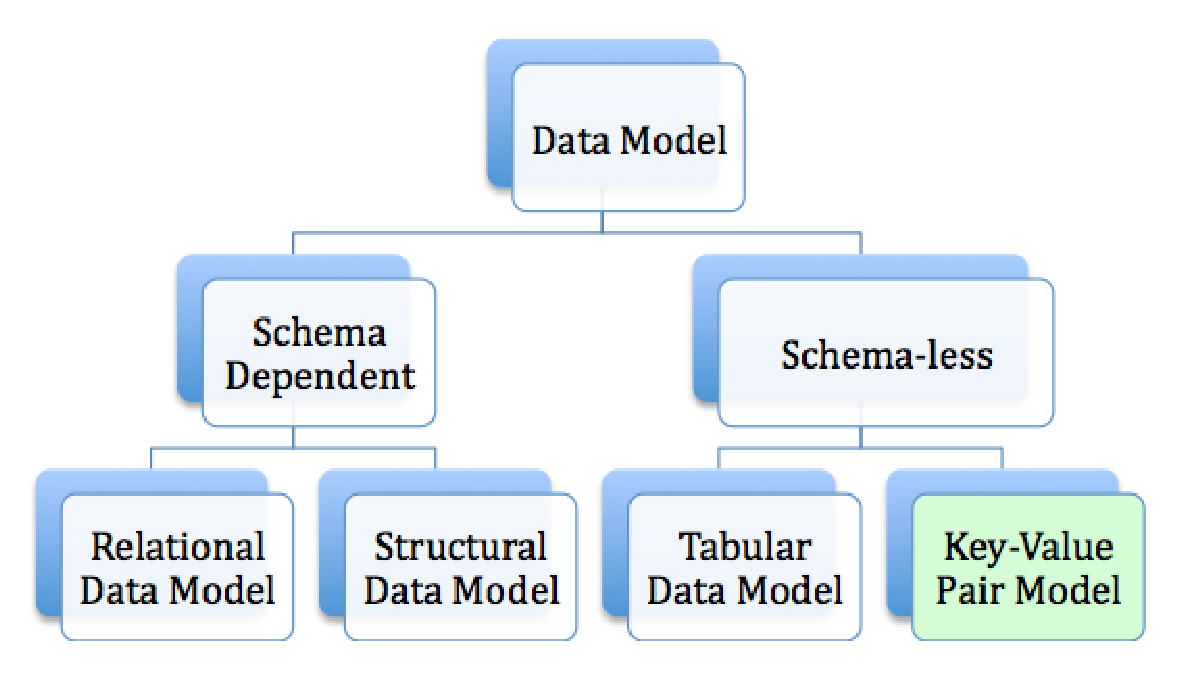
\includegraphics[scale=0.5]{../diagrams/taxonomy-data-model-modified}
  \caption{Data Model Taxonomy}
  \label{fig:taxonomy-data-model-modified}
\end{figure}

Another aspect of the implementation is that provides APIs in different
languages for the data creation and extraction processes. In this way, the
implementation of the persistence model captures the instances of any known
data collected from NetBEAMS and saves it using the document pattern as shown
in Listing \ref{file:mongodb-ysi-data-format}. One application of a
schema-less data model is the addition of any new key-value pair to any
instance of the document, as mongoDB supports update operations to any of the
collections. It can use tags for the purpose of annotations as described in the
taxonomy of data description. For example, in case of an oil spill in the San
Francisco Bay occurs, researchers can update the data set of a given date
range by adding tags to the relating documents. As a consequence of the use of
a schema-less data model, these changes do not affect the other data
instances, since there are no schema changes.

As described in chapter 5, the schema-less data model can provide a better
support to Data Provenance because the data model gives support to the change
of records without affecting the others. In this way, the metadata used by the
implementation clearly describes the three fundamental questions regarding the
collected data from sensor devices, as described in section
\ref{sec:keys-definition}. First, the identity of the data is given by the key
``message\underline{ }id'', in a way that it uniquely identifies the data
produced by the sensor identified by the key ``sensor.ip\underline{
}address''. In this way, the message can be tracked back to the sensor that
produced the data for different purposes such as tracking the data producer.
Second, time dimensions were used in order to track two different aspects of
the data collection: the valid time can be used to correlate observations to
the exact moment it occurred, while the transaction time can be used to verify
when the data was collected, and make decisions such as deleting the instances
of data were collected in the previous two days, etc. Last, but not least, the
use of the key ``sensor.location'' can give the exact location of the data,
since researchers can be interested in finding data based on a specific
location. Finally, the most important aspect of the schema-less data model is
that the observed data is added to the key ``observation'', as any sensor
device carries its set of attributes of key-value pairs. A good example of the
applicability of the schema-less data model is the scalability regarding
changes to the data structure. For instance, if an existing sensor device is
flushed with a new version of the firmware\footnote{The first set of machine
instructions to run on the hardware after the application of power stored
permanently in PROM or ROM or semi-permanently in EPROM}, changing the format
of data types or adding new values, the following instances of collected data
may be different to the previous one by simply adding the new additions of
data. For this reason, the DSP Data Persistence gives administrators the
ability to choose which fields to persist by declaring it using a bootstrap
message for the component, as shown in the parameter ``YSI\underline{
}DESIRED\underline{ }PROPERTIES'' of Listing
\ref{file:dsp-data-persistence-bootstrap.xml}.

The centralized query processing used by NetBEAMS is a result of the
infrastructure used by NetBEAMS, as well as the purpose of data and the
location of the collected data. As a direct result of a schema-less data
model, the centralized query processing is easily developed using any of the
available programming languages provided by mongoDB. Considering the fact that
programming languages are easier abstractions to researchers without computer
science background \cite{sn-programming-language}, mongoDB's approach to data
access through API can be seen as an easier task to manage data. As it is shown
in Listing \ref{file:experiment-query-scenarios}, the scenarios designed to
evaluate the implementation are written in Javascript, since it is the script
language by the mongoDB Shell. Therefore, it attends the requirement of not
using the SQL language as the main query language of the data, giving a better
data access abstraction similar to programming languages for different users.

One of the most important features of a data persistence for sensor
networks is the replacement of the SQL by the use of programming
languages, as they tend to be easier abstraction to users without the
background in database systems \cite{sn-programming-language}. In this way,
mongoDB covers the requirements of providing data access to the collected
sensor data in different languages. For example, the data collected by the DSP
Data Persistence component is written in Java, while the implementation of the
experiments scenarios for querying the collected data is given in Javascript. In
this way, researchers of the RTC may choose one of the enumarated languages
APIs provided by the mongoDB to access the stored data from NetBEAMS.

Finally, the implementation supported by mongoDB during the experiments was
following a single dedicated server virtualization using VirtualBox 
\cite{virtualization}.

\subsection{Infrastructure Evaluation}

Overall, the implementation of the DSP Data Persistence component meets
the specification of the use cases defined in section \ref{sec:exp-scenarios}.
The implementation of mongoDB using a single server environment can give
support to the current workload and infrastructure from the use of NetBEAMS to
collect data from the sensors devices from SF-BEAMS. From the perspective of
disk-space utilization and given that aproximaly 1.3 Gigabytes of disk space
were used to save one year-worth of collected data equivalent to five YSI
devices. According to the mongoDB documentation \ref{mongodb}, the claimed
amount of disk space is related to how mongoDB uses a binary representation
of the JSON documents, which are composed only of strings, together with the
definition of the indexes also represent in JSON. As a consequence, the size of
the keys defined for the YSI sonde data defines the amount of disk space used.
For this reason, different experiments were conducted with different
definitions of the keys of the documents
approach when compared the the RTC's OPEnDAP format shown in Listing
\ref{file:rtc-ysi-opendap}. Then, the second specification used short names
for the keys. In this way, the amount of storage space utilized by for the
different workloads define in section \ref{sec:workload} can be summarized as
follows

The performance to insert data into the database system using the Java driver
is documented by mongoDB as the fastest approach, providing persistence to
approximaly 25,091 documents per minute on an indexed database. In contrast,
when indexes are not used, more then 169,508 documents could be inserted per
minute. Although the latter approach supports more ducuments than the former,
the trade off between insertion and selection time is relevant due to the
activities of retrieval for documents for specific periods of time. Therefore,
the use of indexes might speed the retrieval time considerably. Considering
this number of insertions to the database the number of sensors producing data
and sending to the data sink, mongoDB and NetBEAMS implementation can
virtually support thousands sensor devices.

Disk utilization is one important characteristic of the selected database
system. However, the retrieval of the collected data from sensor devices is
a much more important requirement because most of the utilization of the data
persistence of a sensor network is regarding the search for the properties on
the collected data. After analyzing the response times for the scenarios
described in section \ref{sec:exp-scenarios}, it is clear that the use of
indexes improves the overall execution of the queries, specially because of the
amount of data collected over the years. Furthermore, the response times
described in this scenario is directly related to the use of the External
Storage strategy. On the other hand, improvements over the response time can be
achieved through the implementation of a Data-Centric approach on a Distributed
Database environment, or clusters. In this approach, the inserted data is
stored in different servers based on a partition key. Given the fact that less
data is concentrated in each partition, the centralized query mechanism used is
faster, and consequently improves the performance as described in the Data
Location taxonomy in chapter 3.

When it comes to re-using the data collected by the DSP Data Persistence,
different approaches were available. First, the use of the export capabilities
to a common-delimited values was performed \ref{file:mongodb-export-command},
taking approximaly 3.3 minutes to export one year worth of data for 5 YSI
devices without indexing. Second, the use of the client shell gives a
centralized access to either the single server. However, in order to better
provide access of data to users without skills in database systems, web
applications can be built on top of the REST Web Services APIs \cite{http-rest}
provided by mongoDB. One such example of using the REST API is the adaptation
of Apache Futon 4 mongoDB, as shown in Figure
\ref{fig:view-collections-instance-browser-futondb}, where users can navigate
through the collections of the collected sensor network data categorized by the
collection. Therefore, RTC staff technicians could take advantage of this tool
to view and navigate over the collected data from the sensor devices.

\subsection{Use Cases Evaluation}

Supposing an environmental accident such as the San Francisco oil
  spill happened again \cite{sfbay-oilspill2009}, changing the sampling
  frequency drastically to different values. 

\section{Difficulties Experienced}
\label{sec:experiments-difficulties}
As the development of computing system, the inception of the experiments
described in this chapter had different moments of Software Engineering.
Particularly speaking about the learning curve, different situations
contributed to the success of the first experiments. Since the technoogy is
new, it brought new challenges regarding the usability and user experience.
Since the technology is relatively new and still under development, many
different bugs were could be reproduced by random during the execution of the
experiments, and therefore, sent to the open-source community through use 
different available communication channels. First, the fastest way to solve an
issue was through the mongoDB's IRC channel, located at the Freenode server
(www.freenode.org, channel mongodb). Second, the use of the users group, located
at http://groups.google.com/group/mongodb-user also helped solving problems.

Physical memory is limited, for this reason, it may not be enough to run the
experiments for total workloads. In this case, the Java Virtual Memory was
totally consumed by one of the revisions of the experiments setup. Huge data
loads require different approach to manage data in memory such as creating
object pools as temporary cache for objects whose state are similar to others.

While performing the experiments, the 32bit machine reached its limitation of
2GB of physical data. With know about that, the environment needed to be
updagred for mongoDB requires a 64-bit operating system when the amount of
stored data reaches 2 Gigabytes. For this reason, the scenarios with indexes
used a dedicated virtualized server using Ubuntu Linux 9.04 64 bits with 1 Gb
of memory.
% main.tex, to be used with thesis.tex
% This contains the main work of your thesis.

%\bibliography{thesis}  % uses the references stored in Chapter1Radar.bib

\chapter{Conclusions and Future Works}

This work presented a collection of taxonomies related to data persistence for
sensor networks using different approaches ranging from data models and server
infrastructure organization. The main result of this work was that persistence
for collected data from sensors are better maintained using schema-less data
models, since it provides offers an approach to deal with unanticipated data
types from the sensor devices.

There are many important features covered in this work, including the
importance of the sensor networks rely in how users have access to the
collected data. In order to provide access to the collected data, one must
first assess the different types of infrastructural characteristics of the
studied sensor network. In general, the selection of a technology that
provides such persistence capabilities can be part of a process of analysis of
taxonomies proposed by this work. However, this work proposes a data model not
yet used in the sensor network community and, thus, represents an important
contribution for the area.

Taking into account the software architecture provided by NetBEAMS, as well as
the requirements for data collection from the RTC research group, this work
shows a novice way to persist data collected from sensor devices by using a
schema-less data model, whose query capabilities are based upon programming
languages, in contrast to the use of the Structured Query Language, SQL. The
experiment results showed that the implementation of a persistence layer with
mongoDB can be used to persist data at its maximum rate of one sample per
minute. However, performance can be improved by using techniques such as
database sharding, since it offers a direct implementation capability to
Data-Centric Storage approach. This approach decreases the amount of time to
search data since it distributes the data instances across different cluster
nodes.

There are many different directions for future works. First, the Data-Centric
implementation performance may be extremely improved by using the technique
called MapReduce \cite{map-reduce}. This approach allows mongoDB to search
different machines in parallel whenever the data requested is located in
different database shard hosts. In addition to that, the use techniques to
cluster collected data before they are inserted into the database may be
important as shown in \cite{sn-time-series}. One of the key issues in the
implemented solution is that any measurement of data is considered to be
persisted without further analysis.

All in all, the DSP Data Persistence component implemented for the NetBEAMS
solution to SF-BEAMS can be used in any network server. The solution for data
persistence is a novice way to save data into the database, provided by
mongoDB's ability to cope with the uncertainty of any properties collected from
any sensor specification. Furthermore, the solution also provides a good
support to the provenance-related data.

%% Configuration of the header strings for the Appendices
\renewcommand{\chaptermark}[3]{%
  \markboth{\MakeUppercase{\appendixname\ \thechapter}}%
  {\MakeUppercase{#1}}
}
\appendix
\chapter{Appendix - Source Code / Artifacts}

This section includes the source-code for the DSP Data Persistence. Each
section details one single main artifact used on the development of the
component. However, only the main ones will be added into this document, while
the remainder can be downloaded directly from the Subversion repository.

The source code is located in the Subversion repository for the NetBEAMS
project. This is how it is structured:

\section{DSP Data Persistence Component}

This artifact defines the ANT build file.

\lstinputlisting[language=Ant,label=file:dsp-build.xml,caption=Build
system using Apache ANT]{../../../../netbeams/versions/v2/apps/osgi-bundles/dsp/DSPDataPersistence/build.xml}

%\lstinputlisting[language=bash,label=file:osgi-manifest,caption=OSGi
%Manifest
%Descriptor]{../../../../netbeams/versions/v2/apps/osgi-bundles/dsp/DSPDataPersistence/META-INF/MANIFEST.MF}

\lstinputlisting[language=XML,label=file:dsp-config.xml,caption=DSP
Deployment
Configuration]{../../../../netbeams/versions/v2/config/deployment/config.xml}

\lstinputlisting[language=XML,label=file:dsp-matcher-config.xml,caption=DSP
Matching Rules]{../../../../netbeams/versions/v2/config/deployment/matcher_config.xml}

\lstinputlisting[language=XML,label=file:dsp-matcher-config-gumstix.xml,caption=DSP
Matching Rules
for
Gumstix]{../../../../netbeams/versions/v2/config/deployment/matcher_config-gumstix.xml}

%TODO: add bootstrap message in case it is implemented

\lstinputlisting[language=Java,label=file:dsp-activator,caption=OSGi
Activator]{../../../../netbeams/versions/v2/apps/osgi-bundles/dsp/DSPDataPersistence/src/org/netbeams/dsp/persistence/osgi/DataPersistenceActivator.java}

\lstinputlisting[language=Java,label=file:dsp-component-service,caption=OSGi
Service - Component]{../../../../netbeams/versions/v2/apps/osgi-bundles/dsp/DSPDataPersistence/src/org/netbeams/dsp/persistence/controller/DSPDataPersistence.java}

\lstinputlisting[language=Java,label=file:dsp-mongo-service,caption=DSP Data to
Mongo DB
Service]{../../../../netbeams/versions/v2/apps/osgi-bundles/dsp/DSPDataPersistence/src/org/netbeams/dsp/persistence/controller/DSPMongoCRUDService.java}

\lstset{language=XML,morecomment=[s]{!--}{--},label=file:dsp-message-serialized-ysi,caption=DSP
Message with a YSI sonde data payload}
\begin{lstlisting}
<?xml version="1.0" encoding="UTF-8" standalone="yes"?>
<MessagesContainer uudi="24929c29-60ee-4d17-af08-64d9446277ef"
        creationTime="2009-03-06T15:17:18-0800" destinationHost="192.168.0.106">
   <MeasureMessage ContentType="org.netbeams.dsp.ysi"
         messageID="435a61f6-370f-458d-aeb7-6e92270a79cb">
      <Header>
         <CreationTime>1236381438480</CreationTime>
         
         <Producer>   
            <ComponentType>
                 org.netbeams.dsp.platform.management.component.ComponentManager
            </ComponentType>
            
            <ComponentLocator>
               <ComponentNodeId>1234</ComponentNodeId>
               <NodeAddress>192.168.0.103</NodeAddress>
            </ComponentLocator>
         </Producer>
         
         <Consumer>
            <ComponentType>
                 org.netbeams.dsp.wiretransport.client
            </ComponentType>
            
            <ComponentLocator>
               <NodeAddress>LOCAL</NodeAddress>
            </ComponentLocator>
         </Consumer>
      </Header>
      <Body>
         <SondeDataContainer>
            <soundeData date="15:17:18" time="03-06-2009">  
               <Temp>21.20</Temp>
               <SpCond>193</SpCond>
               <Cond>179</Cond>
               <Resist>5588.40</Resist>
               <Sal>0.09</Sal>
               <Press>0.084</Press>
               <Depth>0.059</Depth>
               <pH>7.98</pH>
               <phmV>-79.6</phmV>
               <ODOSat>99.5</ODOSat>
               <ODOConc>8.83</ODOConc>
               <Turbid>0.4</Turbid>
               <Battery>8.7</Battery>
            </soundeData>
         </SondeDataContainer>
      </Body>
   </MeasureMessage>
</MessagesContainer>
\end{lstlisting}

\section{Experiment Implementation}

\lstinputlisting[language=Bash,label=file:experiment-setup-executor,caption=Experiment
Implementation]{../../../../netbeams/versions/v2/persistence/run-persistence-experiment}

\lstinputlisting[language=Java,label=file:experiment-dsp-implementation,caption=Experiment
Implementation]{../../../../netbeams/versions/v2/apps/osgi-bundles/dsp/DSPDataPersistence/src/org/netbeams/dsp/persistence/controller/DSPMessageToMongoDBExperiment.java}

\lstset{label=file:mongodb-ysi-data-format,caption=JSON representation of the
data produced by a YSI sensor on mongoDB}
\begin{lstlisting}
            {
             "_id" :  ObjectId( "d36f4007b7e7ac4a03c60000")  , 
             "sensor_ip_address" : "192.168.0.136", 
             "message_id" : "7b6624d6-0ca1-4cba-a343-f166e88da73b",
             "transaction_time" : 1252845473412 , 
             "fact_time" : 1252845346000,
             "latitude" : 12.3450, 
             "longitude" : -123.4456 , 
             "data" : {
                       "temperature" : 45.01, 
                       "sp_condition" : 37.6, 
                       "condition" : 145.8, 
                       "resistence" : 159.77, 
                       "salinitude" : 0.0, 
                       "pressure" : 0.391, 
                       "depth" : 0.46, 
                       "ph" : 5.64, 
                       "pH_mv" : -62.1, 
                       "odo_sat" : 89.7, 
                       "odo_condition" : 59.34, 
                       "turbidity" : 0.0,
                       "battery" : 9.4
                      }
            }
\end{lstlisting}

\lstset{label=file:rtc-ysi-opendap,caption=HTTP GET Request x Response to the OPeNDAP server at SF-BEAMS}
\begin{lstlisting}
http://sfbeams.sfsu.edu:8080/opendap/sfbeams/data_ctd/rtc_ctd5-ysimoor/real-time/sfb_CTD5_PUF.dat.ascii?
GET /opendap/sfbeams/data_ctd/rtc_ctd5-ysimoor/real-time/sfb_CTD5_PUF.dat.dods?&Month=11&Day=12 HTTP/1.1

HTTP/1.x 200 OK
Server: Apache-Coyote/1.1
Last-Modified: Thu, 12 Nov 2009 17:55:06 GMT
XDODS-Server: Server-Version-Unknown
XOPeNDAP-Server: bes/3.5.1 freeform_handler/3.7.5, netcdf_handler/3.7.6
XDAP: 3.2
Content-Description: dods_data
Content-Type: text/txt
Date: Sun, 15 Nov 2009 03:08:45 GMT

Dataset: sfb_CTD5_PUF.dat
YSI_REALTIME_CSV.Month, YSI_REALTIME_CSV.Day, YSI_REALTIME_CSV.Year, YSI_REALTIME_CSV.Hour, YSI_REALTIME_CSV.Min, YSI_REALTIME_CSV.Sec, YSI_REALTIME_CSV.WaterTemperature, YSI_REALTIME_CSV.SpecificConductivity, YSI_REALTIME_CSV.Conductivity, YSI_REALTIME_CSV.Resistivity, YSI_REALTIME_CSV.TDS, YSI_REALTIME_CSV.Salinity, YSI_REALTIME_CSV.Pressure, YSI_REALTIME_CSV.Depth, YSI_REALTIME_CSV.pH, YSI_REALTIME_CSV.pHmV, YSI_REALTIME_CSV.Turbidity, YSI_REALTIME_CSV.ODOSaturation, YSI_REALTIME_CSV.ODO, YSI_REALTIME_CSV.Chlor, YSI_REALTIME_CSV.Chlor_RFU, YSI_REALTIME_CSV.Battery, YSI_REALTIME_CSV.InstSN
11, 12, 2009, 16, 30, 51, 13.78, 4.3945, 3.4532, 0, 28.56, 28.35, 2.65, 2.651, 7.9, -54.7, 9, -99999, -99999, 3.7, 1, 9.4, -99999
11, 12, 2009, 16, 36, 50, 13.78, 4.4095, 3.4642, 0, 28.66, 28.46, 2.628, 2.63, 7.91, -54.9, 11.9, -99999, -99999, 4, 1.1, 9.4, -99999
11, 12, 2009, 16, 42, 51, 13.77, 4.3943, 3.4515, 0, 28.56, 28.35, 2.631, 2.632, 7.9, -54.9, 9.8, -99999, -99999, 3.6, 1, 9.4, -99999
11, 12, 2009, 16, 48, 50, 13.76, 4.3893, 3.447, 0, 28.53, 28.32, 2.628, 2.63, 7.9, -54.8, 10.6, -99999, -99999, 3.8, 1, 9.4, -99999
\end{lstlisting}



% Bibliography (calls up the entries in thesis.bib if you run bibTeX):
%http://www.semaprojects.net/resources/latex/bibtex-styles/
%\bibliographystyle{plainnat}
\bibliographystyle{alpha}
\addcontentsline{toc}{chapter}{Bibliography}
\singlespacing
\bibliography{thesis}

\end{document}
